\section{Esempi di utilizzo}
Ultimata l'implementazione del metodo è bene spendere del tempo per testarne l'efficacia ed osservare come i vari parametri influenzano i risultati ottenuti.\\
Richiamiamo il significato teorico dei vari parametri:
\begin{itemize}
    \item num\_iter (numero di iterazioni per il metodo di Eulero): maggiore è il valore di questo parametro e più volte verrà applicato il metodo
    \item delta\_t (costante d'integrazione): maggiore è il valore di questo parametro e maggiore sarà l'intensità con cui viene applicato il metodo\\
    \item c (coefficiente di controllo del gradiente): permette di far risaltare di più (se c<1) o di meno (se c>1) i bordi
    \item sigma (costante di controllo diffusione uniforme): il calcolo del vettore c utilizzato per modificare l'equazione del calore avviene tramite gradiente. Come già analizzato nella sezione 5.3, conviene fare questo calcolo su una versione sfocata dell'immagine, per fare ciò applichiamo l'equazione del calore. Modificarne questo coefficiente significa modificare l'intensità con cui viene applicata. Un valore più alto sfoca di più e porta ad eliminare più rapidamente il rumore a discapito della definizione dei bordi.
\end{itemize}
Definiremo dei parametri che andranno a costituire il nostro standard ed apporteremo delle modifiche per vedere chiaramente la differenza tra i risultati ottenuti.
Vediamo quindi alcuni esempi.

\newpage
\subsection{Esempio 1 - Risultati ottenuti con i parametri standard}
Vediamo innanzitutto degli esempi di casi reali, Vediamo come operano i due filtri implementati con i parametri mostrati nel codice alla fine dello scorso capitolo\\
Parametri:
\begin{itemize}
    \item num\_iter=20
    \item delta\_t=0.1
    \item c=60
    \item sigma=1
\end{itemize}

\begin{figure}[htb] \centering
%\includegraphics[scale=0.13]{Pictures/Esempi di utilizzo/Esempio 1/Amira_originale.png}
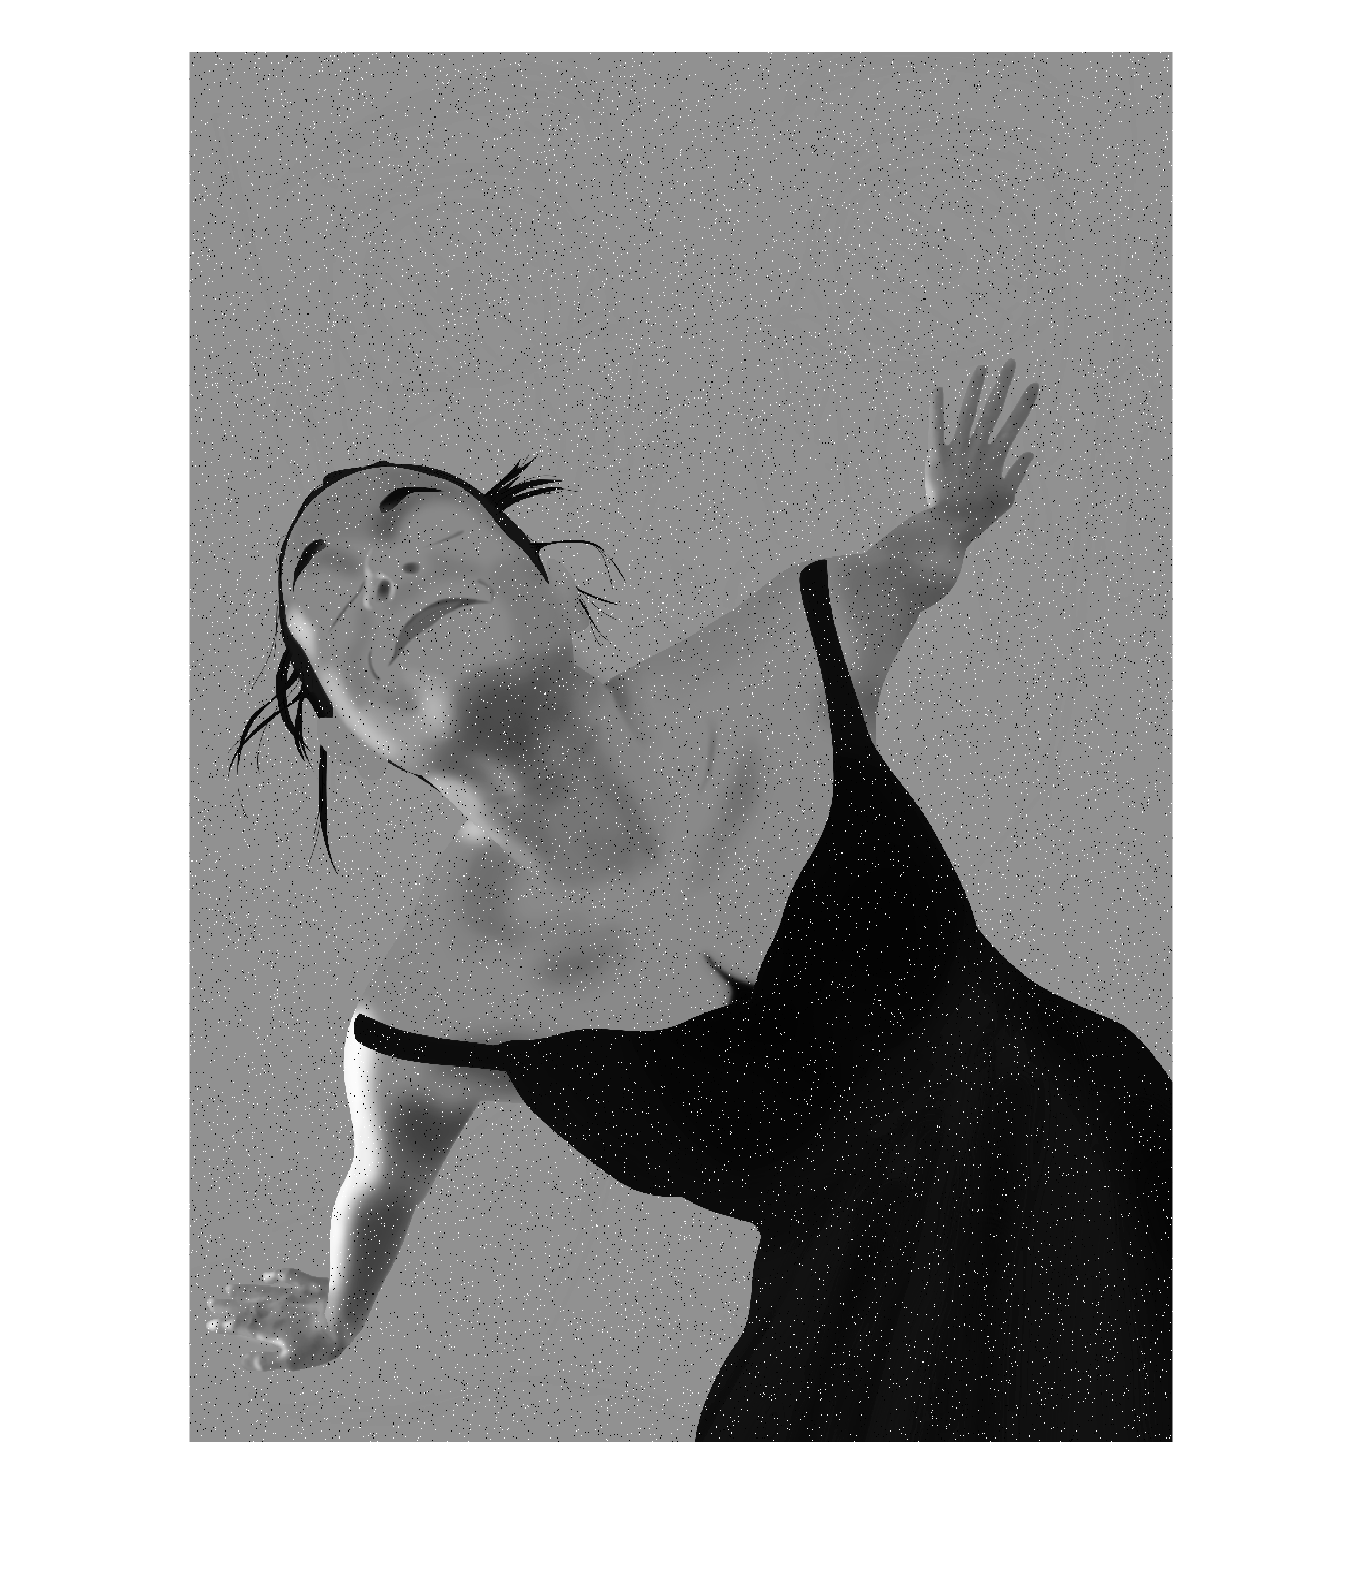
\includegraphics[scale=0.13,trim={6cm 0 4.5cm 0},clip]{Pictures/Esempi di utilizzo/Esempio 1/Amira_con_rumore.png}
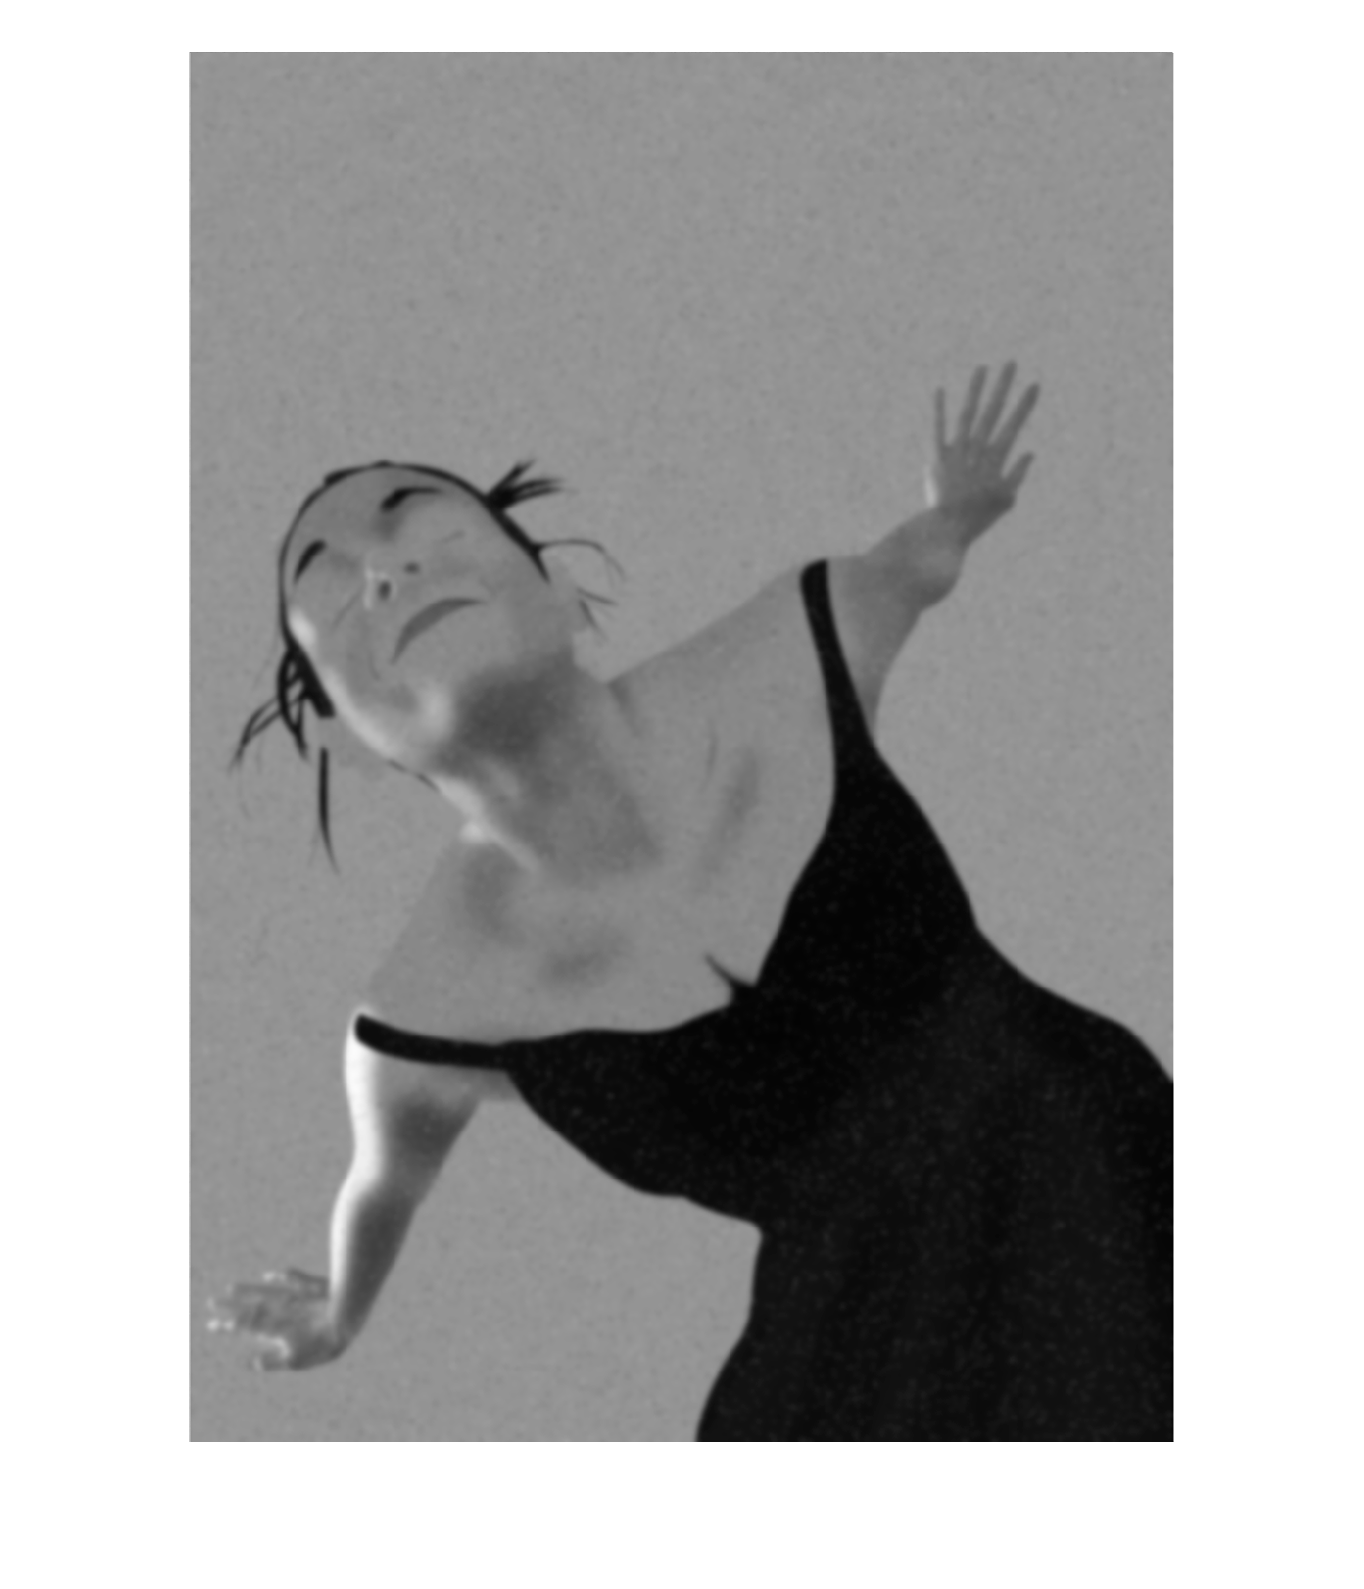
\includegraphics[scale=0.13,trim={6cm 0 6cm 0},clip]{Pictures/Esempi di utilizzo/Esempio 1/Amira_diffusa.png}
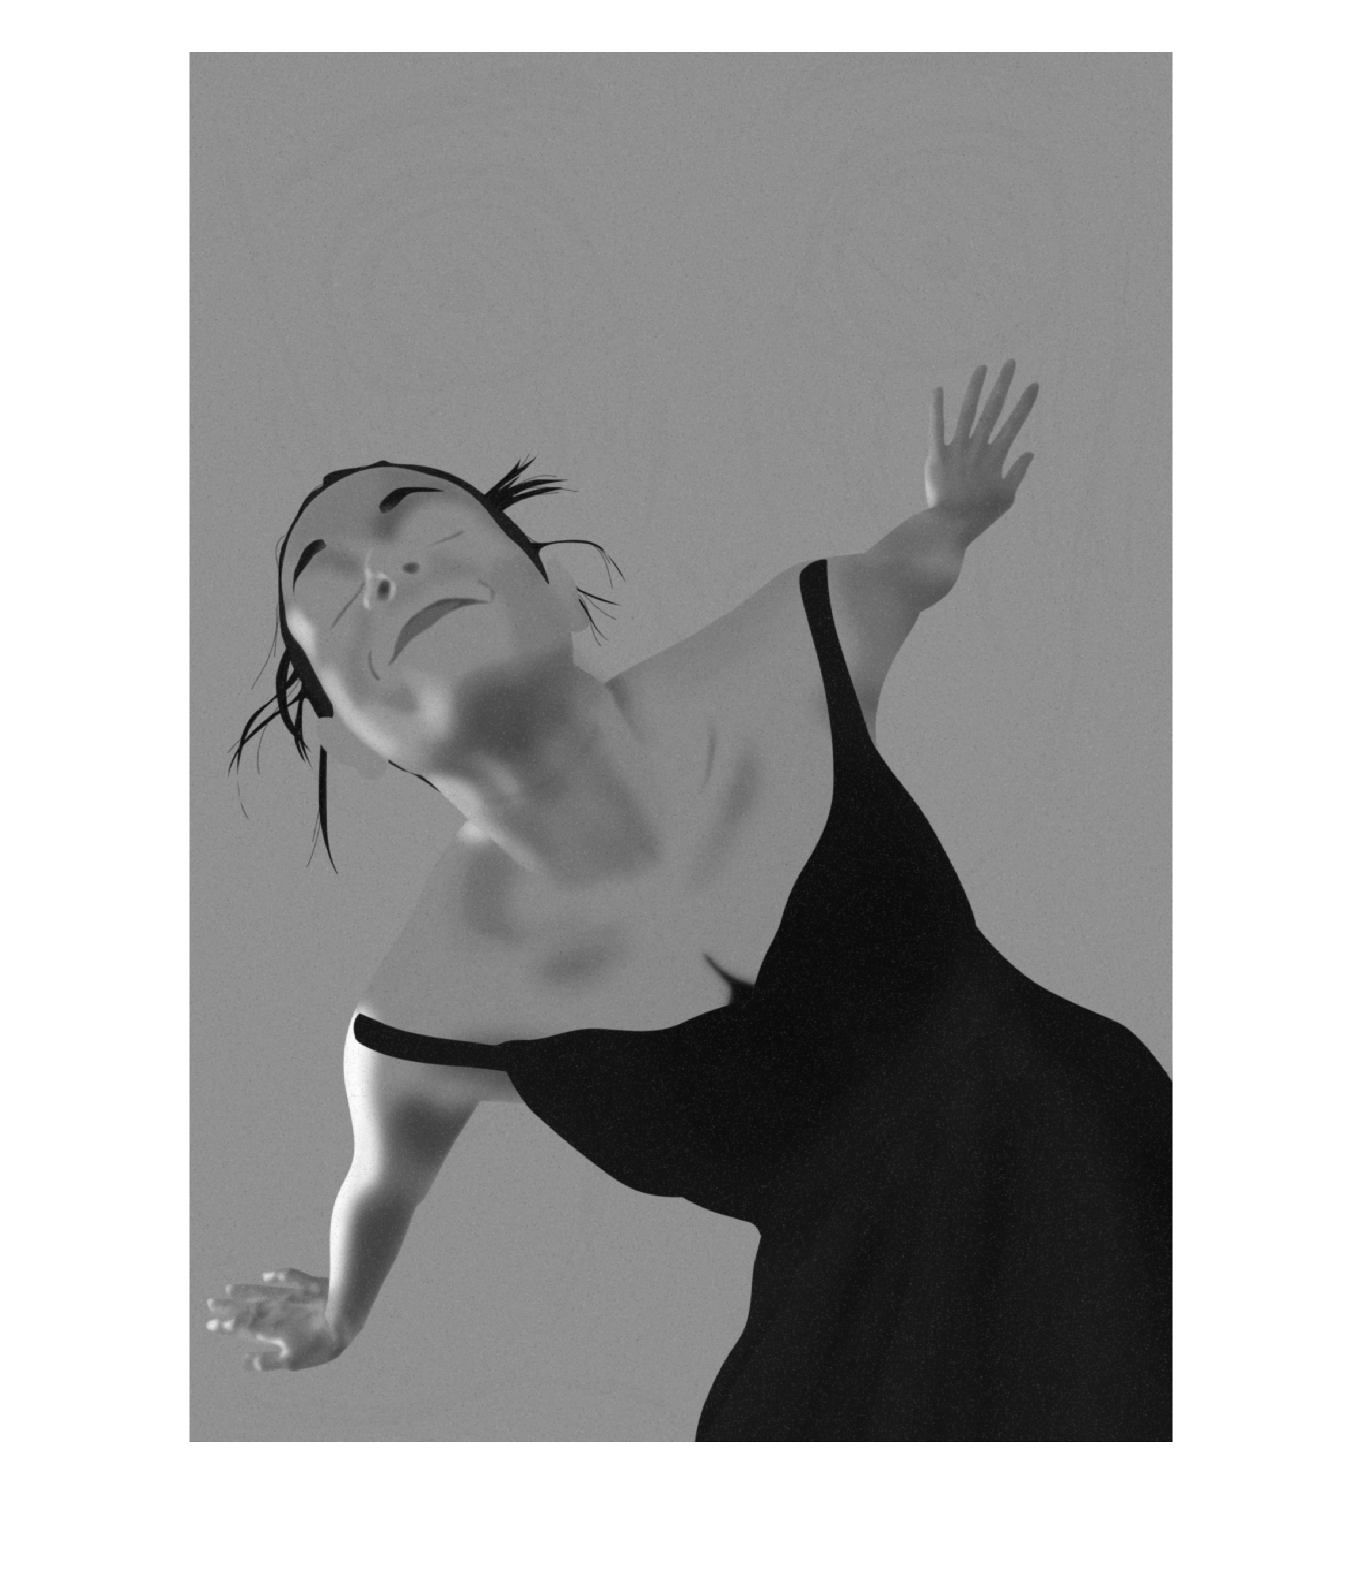
\includegraphics[scale=0.13,trim={4.5cm 0 6cm 0},clip]{Pictures/Esempi di utilizzo/Esempio 1/Amira_filtrata.png}
\caption{Da sinistra a destra: immagine con rumore, immagine filtrata con equazione del calore e immagine filtrata con metodo Perona-Malik.}\label{fig:figura}
\end{figure} 
Per brevità d'ora in avanti ci riferiremo a questi parametri come parametri standard.

\newpage
\subsection{Esempio 2 - Variazione del numero di iterazioni}
Andiamo adesso a vedere come il numero di iterazioni influisce sul risultato\\
filtriamo la stessa immagine confrontando i risultati dopo 10 iterazioni, dopo 20 iterazioni (valore standard) e dopo 100 iterazioni.
Parametri:
\begin{itemize}
    \item num\_iter=10, 20, 100
    \item delta\_t=0.1
    \item c=60
    \item sigma=1
\end{itemize}

\begin{figure}[htb] \centering
%\includegraphics[scale=0.13]{Pictures/Esempi di utilizzo/Amira_originale.png}
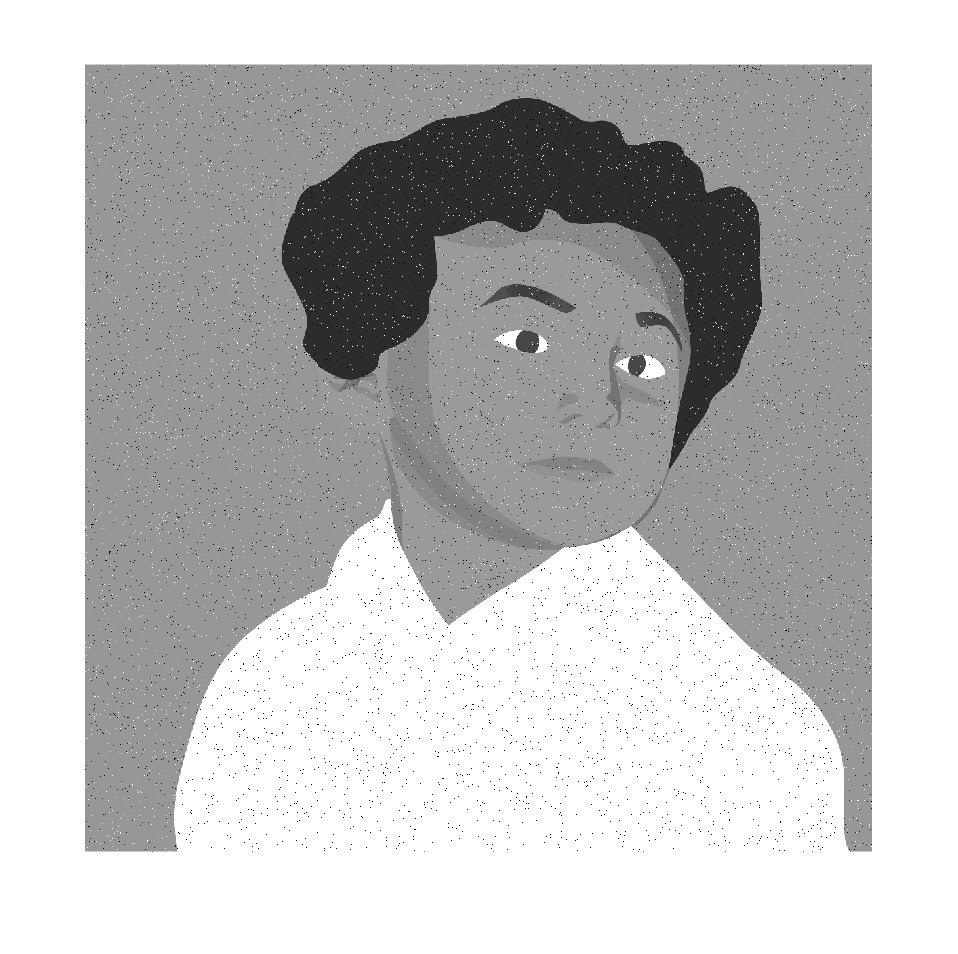
\includegraphics[scale=0.25]{Pictures/Esempi di utilizzo/Esempio 2/raffo_originale.png}
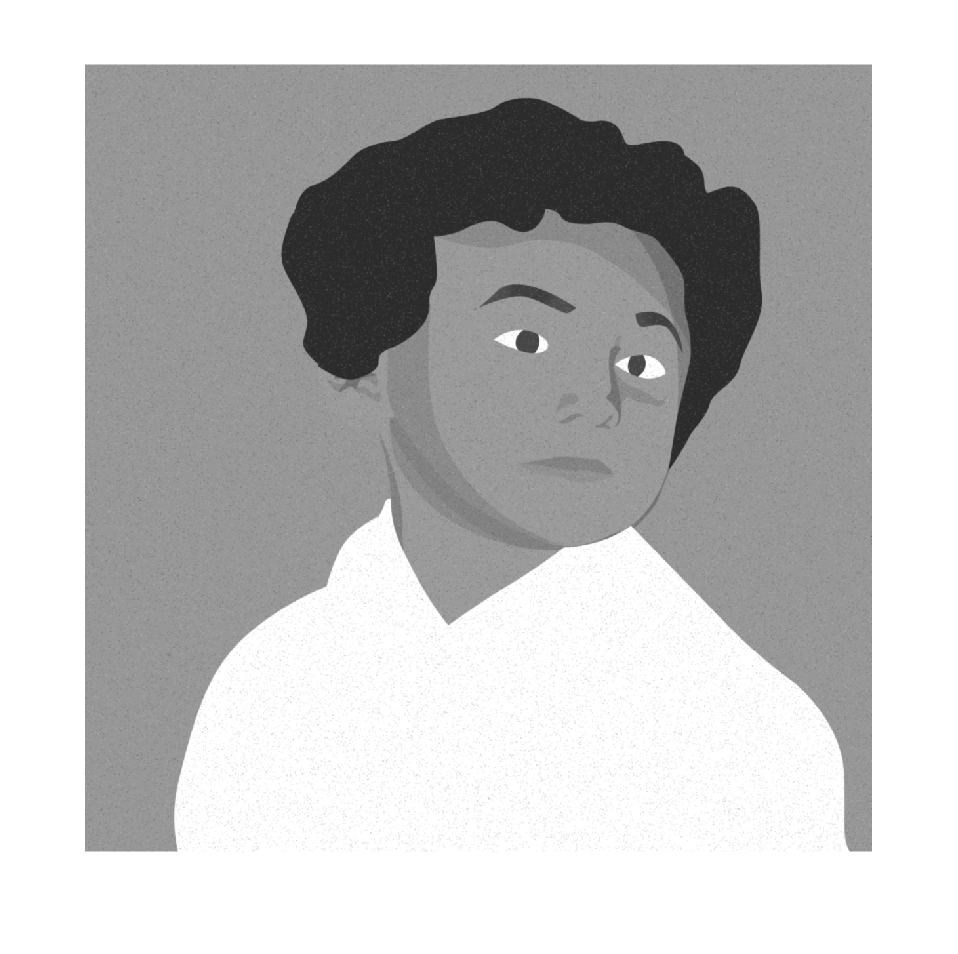
\includegraphics[scale=0.25]{Pictures/Esempi di utilizzo/Esempio 2/raffo_filtrata_n_iter10.png}
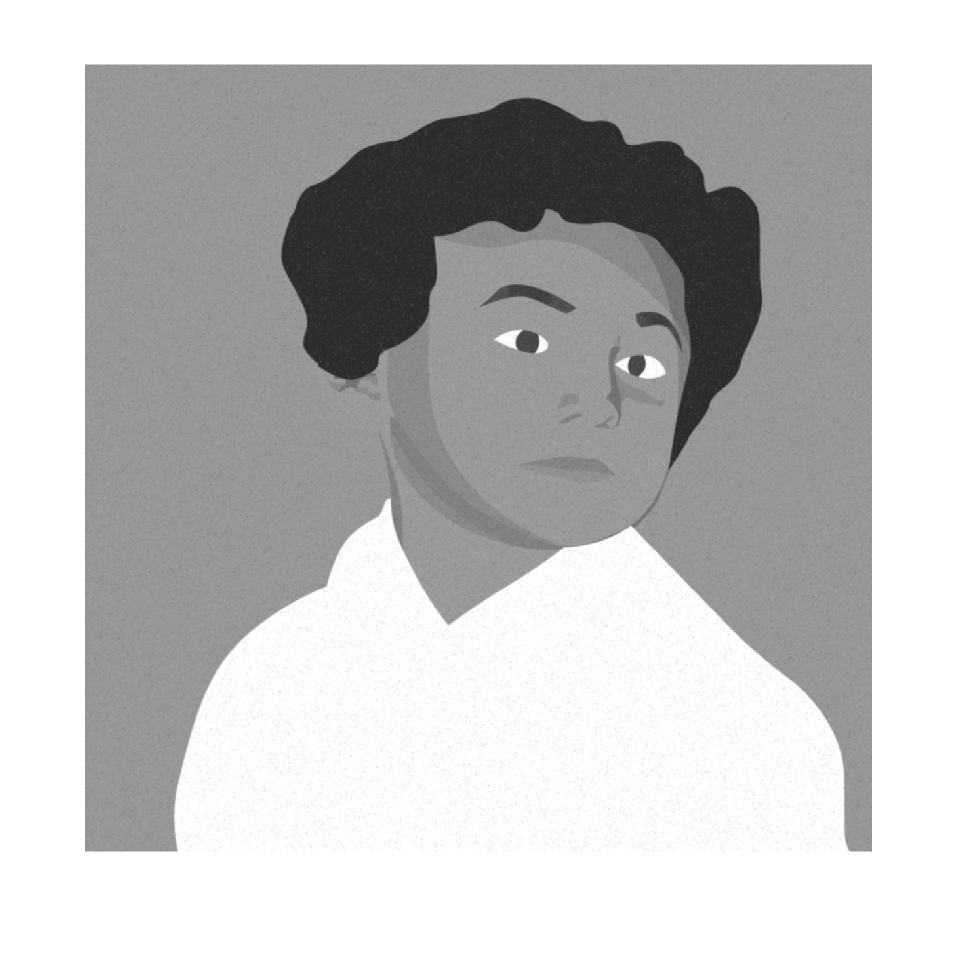
\includegraphics[scale=0.25]{Pictures/Esempi di utilizzo/Esempio 2/raffo_filtrata_n_iter20.png}
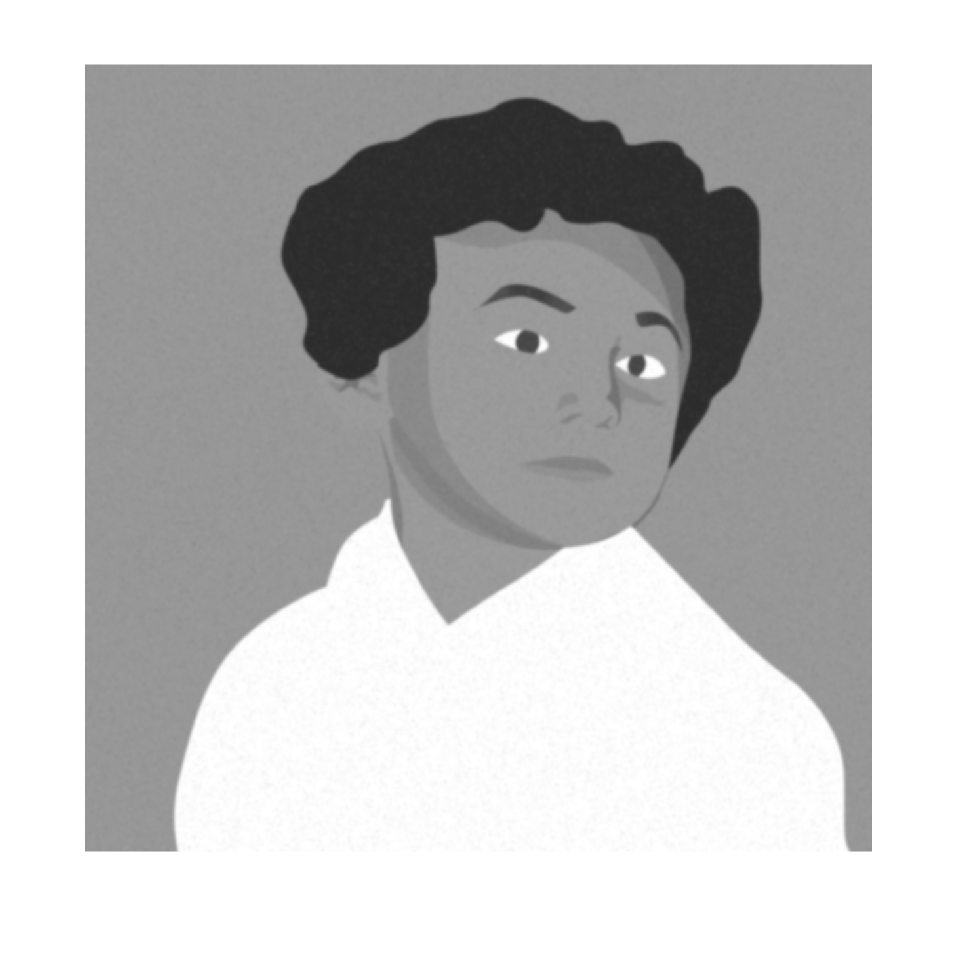
\includegraphics[scale=0.25]{Pictures/Esempi di utilizzo/Esempio 2/raffo_filtrata_n_iter100.png}
\caption{In ordine: immagine con rumore e immagine filtrata dopo 10 iterazioni, dopo 20 iterazioni e dopo 100 iterazioni.}\label{fig:figura}
\end{figure} 
Per poter meglio apprezzare le differenze vediamo delle sezioni d'immagine\\

\begin{figure}[htb] \centering
%\includegraphics[scale=0.13]{Pictures/Esempi di utilizzo/Amira_originale.png}
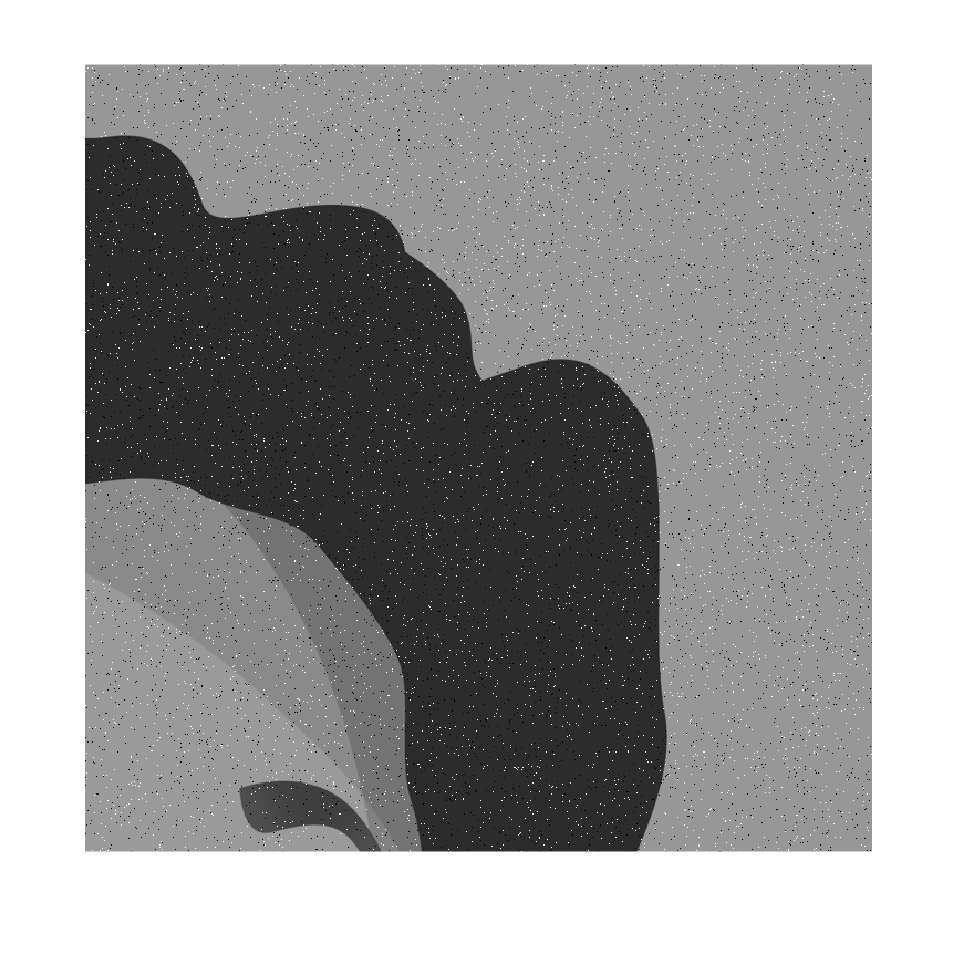
\includegraphics[scale=0.25]{Pictures/Esempi di utilizzo/Esempio 2/raffo_originale_dettaglio.png}

\includegraphics[scale=0.25]{Pictures/Esempi di utilizzo/Esempio 2/raffo_filtrata_n_iter10_dettaglio.png}

\includegraphics[scale=0.25]{Pictures/Esempi di utilizzo/Esempio 2/raffo_filtrata_n_iter20_dettaglio.png}

\includegraphics[scale=0.25]{Pictures/Esempi di utilizzo/Esempio 2/raffo_filtrata_n_iter100_dettaglio.png}
\caption{In ordine: immagine con rumore e immagine filtrata dopo 10 iterazioni, dopo 20 iterazioni e dopo 100 iterazioni.}\label{fig:figura}
\end{figure} 
Tramite queste immagini possiamo apprezzare come ad ogni ulteriore iterazione il rumore venga ridotto, rovinando tuttavia i bordi. \'E dunque bene valutare quando sia il caso di aumentare il numero di iterazioni e quando no. Se l'immagine in esame presenta dei bordi molto marcati, come ad esempio una scritta converrà preservarli il più possibile. Al contrario se l'immagine è caratterizzata per lo più da sfocature ci si può concedere di aumentare il numero di iterazioni.\\
\'E bene ricordare però che aumentare il numero di iterazioni porta un notevolmente aumento del costo computazionale e dunque del tempo di elaborazione.

\newpage
\subsection{Esempio 3 - Variazione della costante d'integrazione}
Passiamo ora alla costante d'integrazione e come cambiarla influisca con i risultati.\\
Parametri:
\begin{itemize}
    \item num\_iter=20
    \item delta\_t=0.01, 0.1, 0.2
    \item c=60
    \item sigma=1
\end{itemize}

\begin{figure}[htb] \centering
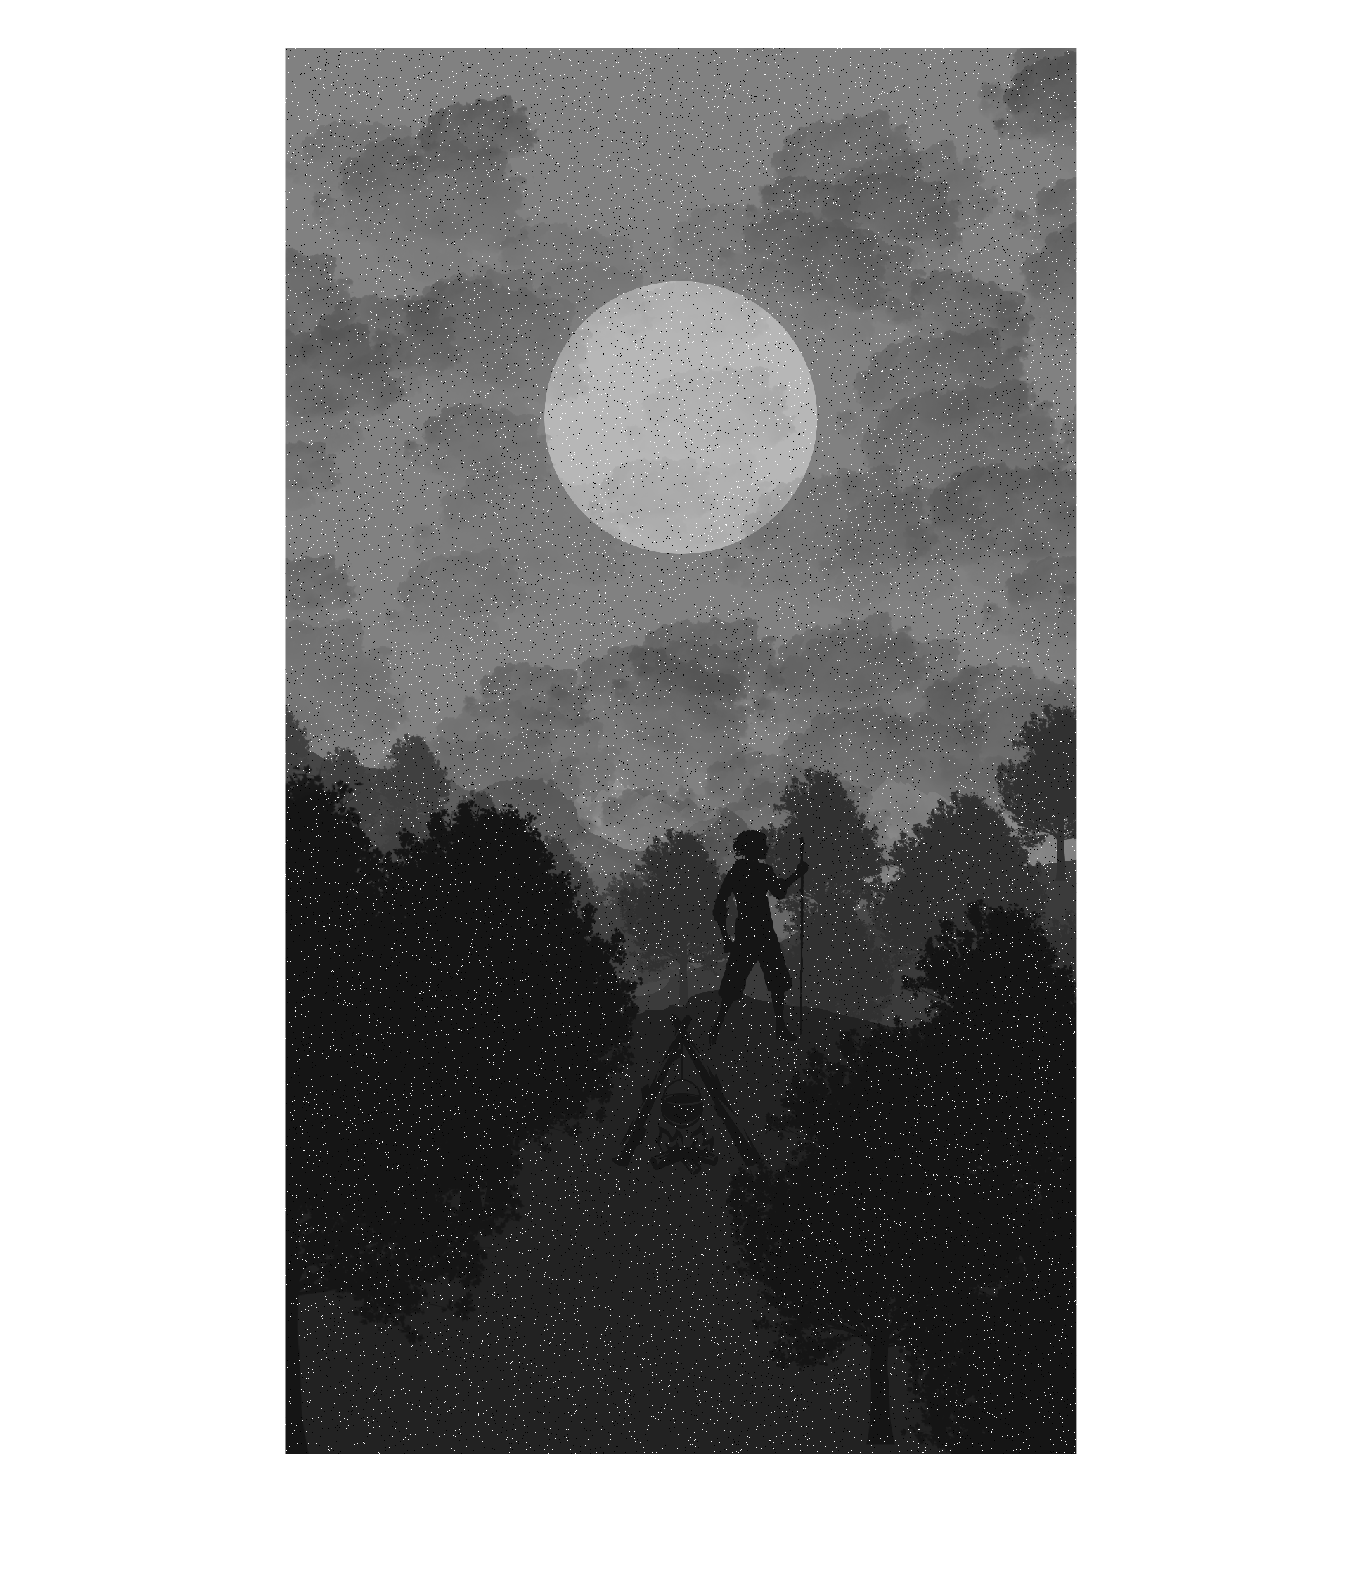
\includegraphics[scale=0.15]{Pictures/Esempi di utilizzo/Esempio 3/SfondoForesta_con_rumore.png}
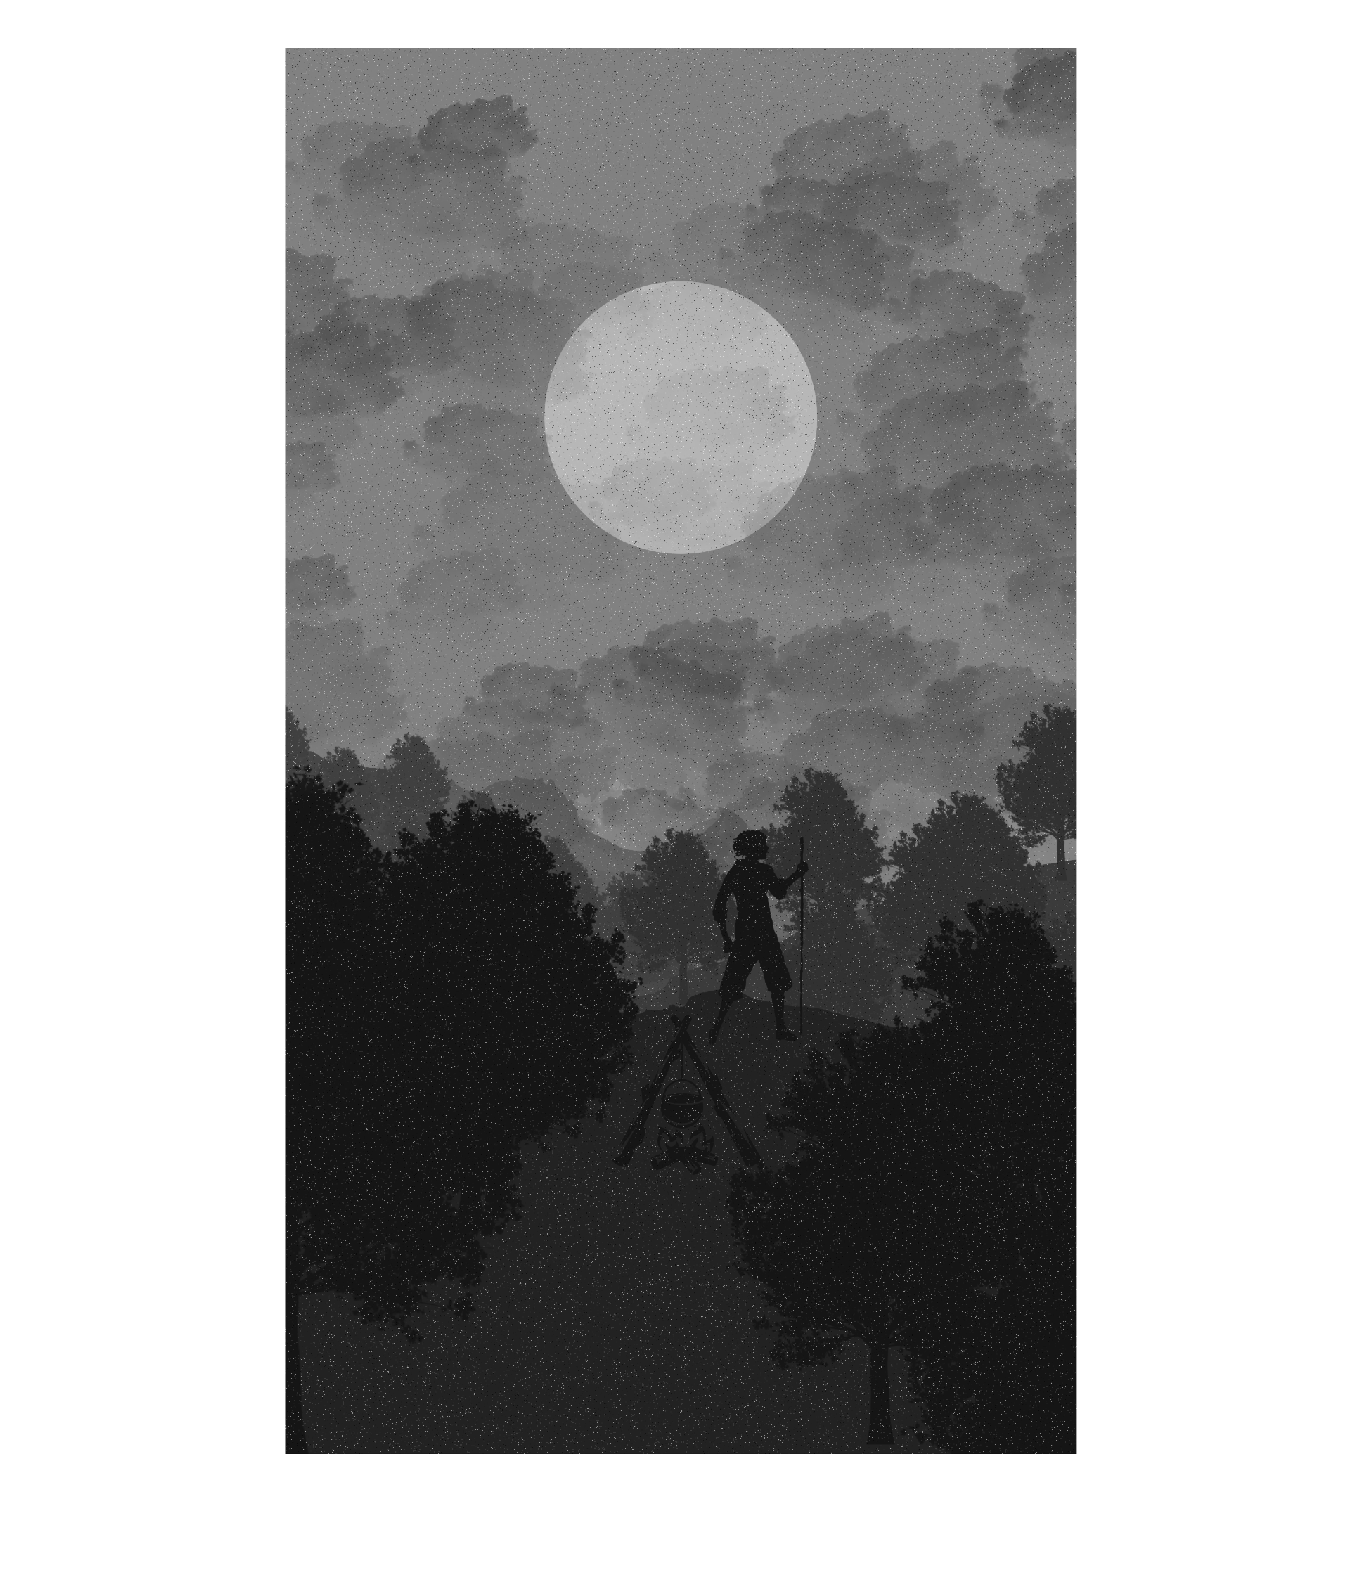
\includegraphics[scale=0.15]{Pictures/Esempi di utilizzo/Esempio 3/SfondoForesta_filtrata_deltat0_01.png}
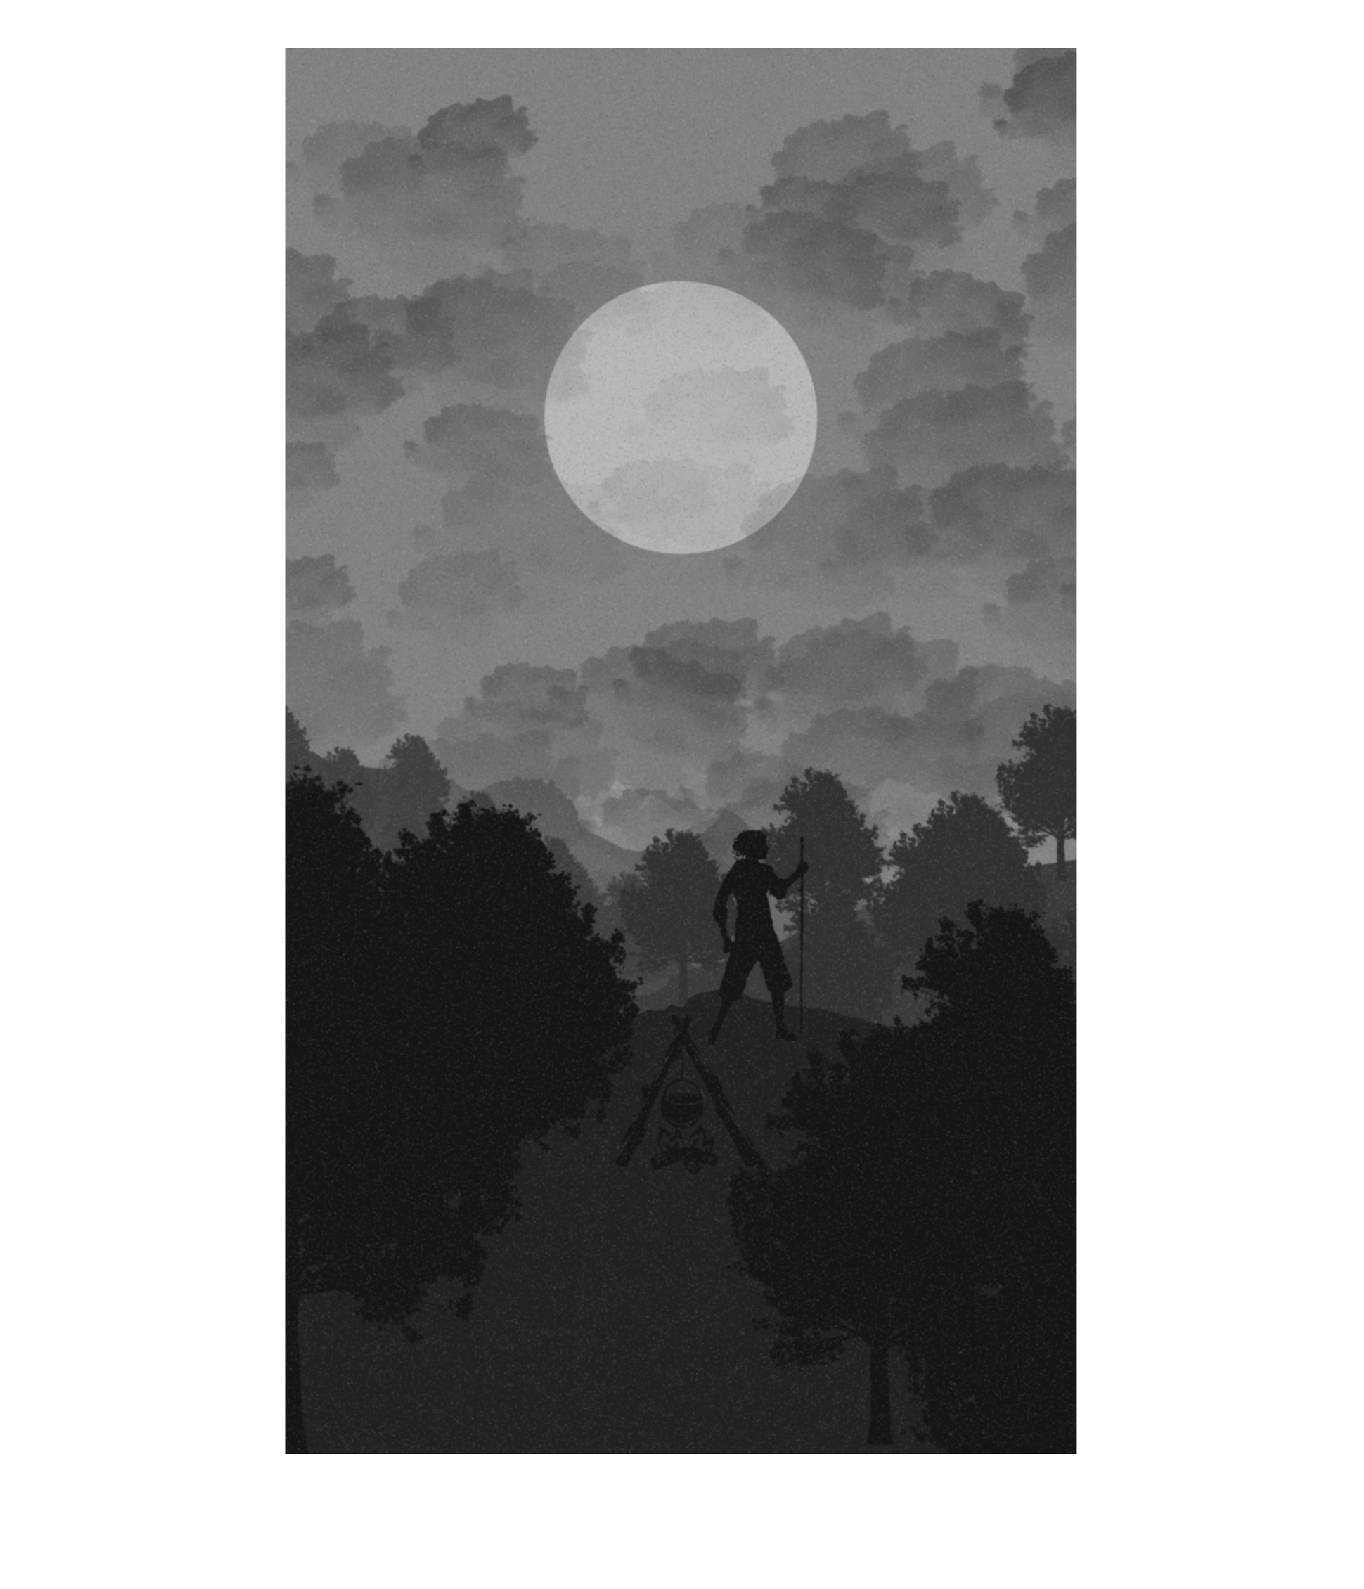
\includegraphics[scale=0.15]{Pictures/Esempi di utilizzo/Esempio 3/SfondoForesta_filtrata_deltat0_1.png}
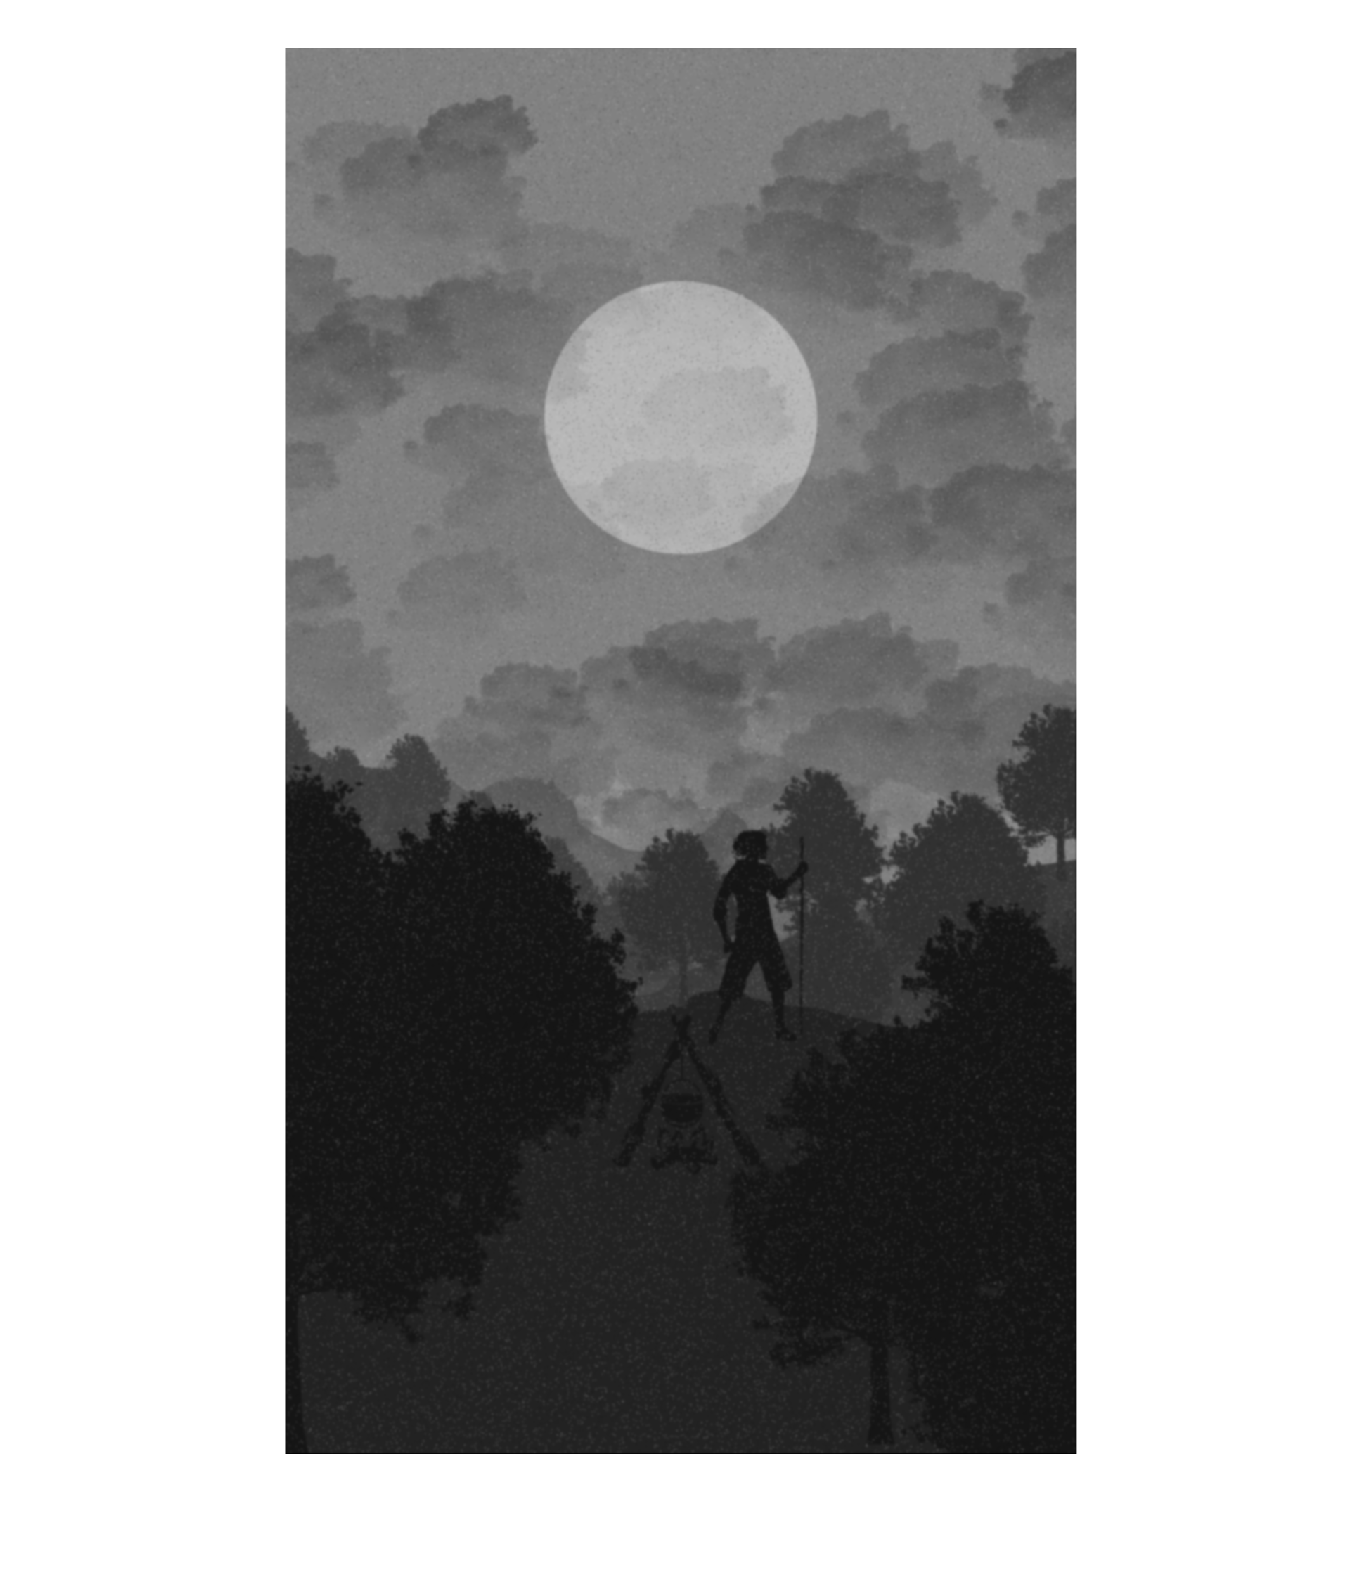
\includegraphics[scale=0.15]{Pictures/Esempi di utilizzo/Esempio 3/SfondoForesta_filtrata_deltat0_25.png}
\caption{In ordine: immagine con rumore, immagine filtrata con delta\_t=0.01, con delta\_t=0.1 e con delta\_t=0.25.}\label{fig:figura}
\end{figure} 
Da queste immagini è chiaramente visibile che per delta\_t prossimo allo zero (in questo caso 0.01) il problema del rumore non viene risolto, Ma solo attenuato. d'altro canto aumentandone il valore si perdono informazioni sui bordi molto più velocemente. Per poter meglio apprezzare questa differenza guardiamo delle sezioni delle ultime due immagini\\

\begin{figure}[htb] \centering
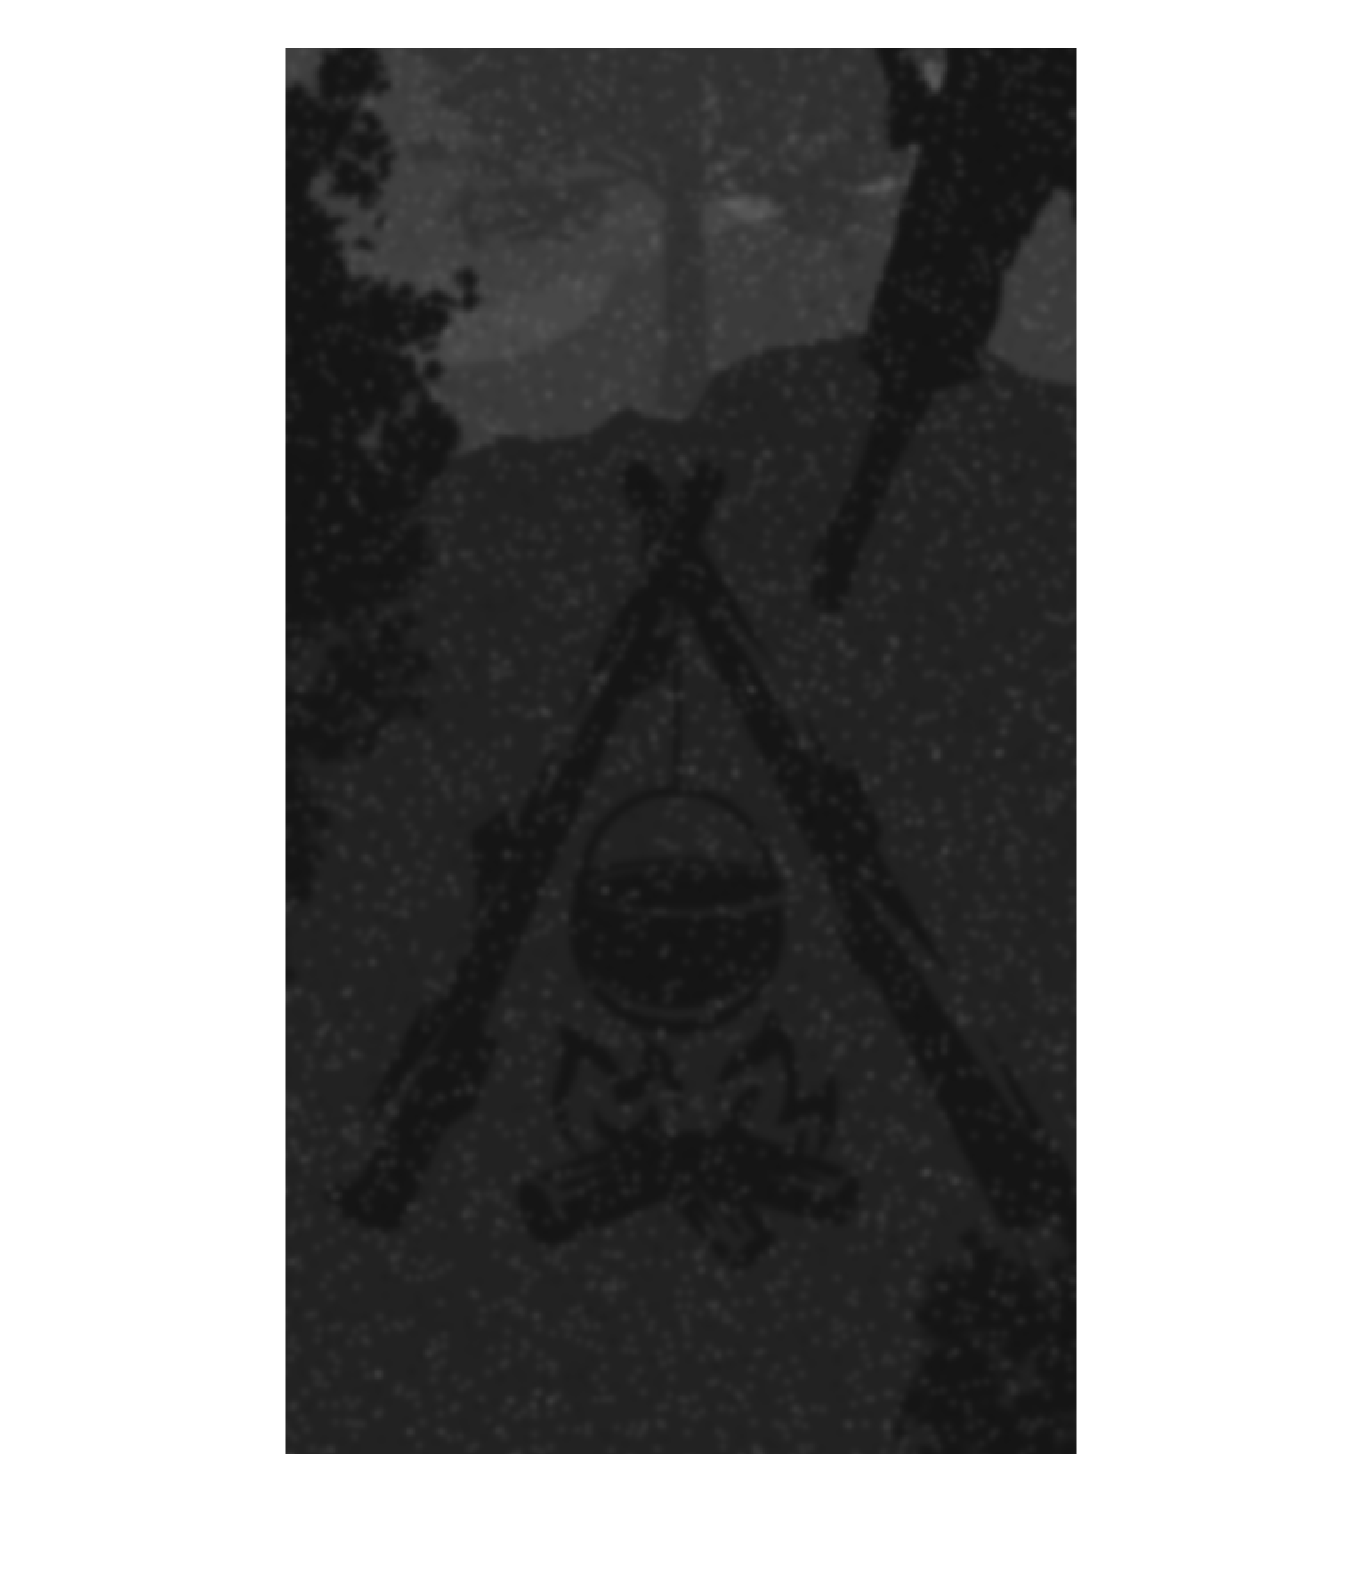
\includegraphics[scale=0.15]{Pictures/Esempi di utilizzo/Esempio 3/Dettaglio_SfondoForesta_filtrata_deltat0_1.png}
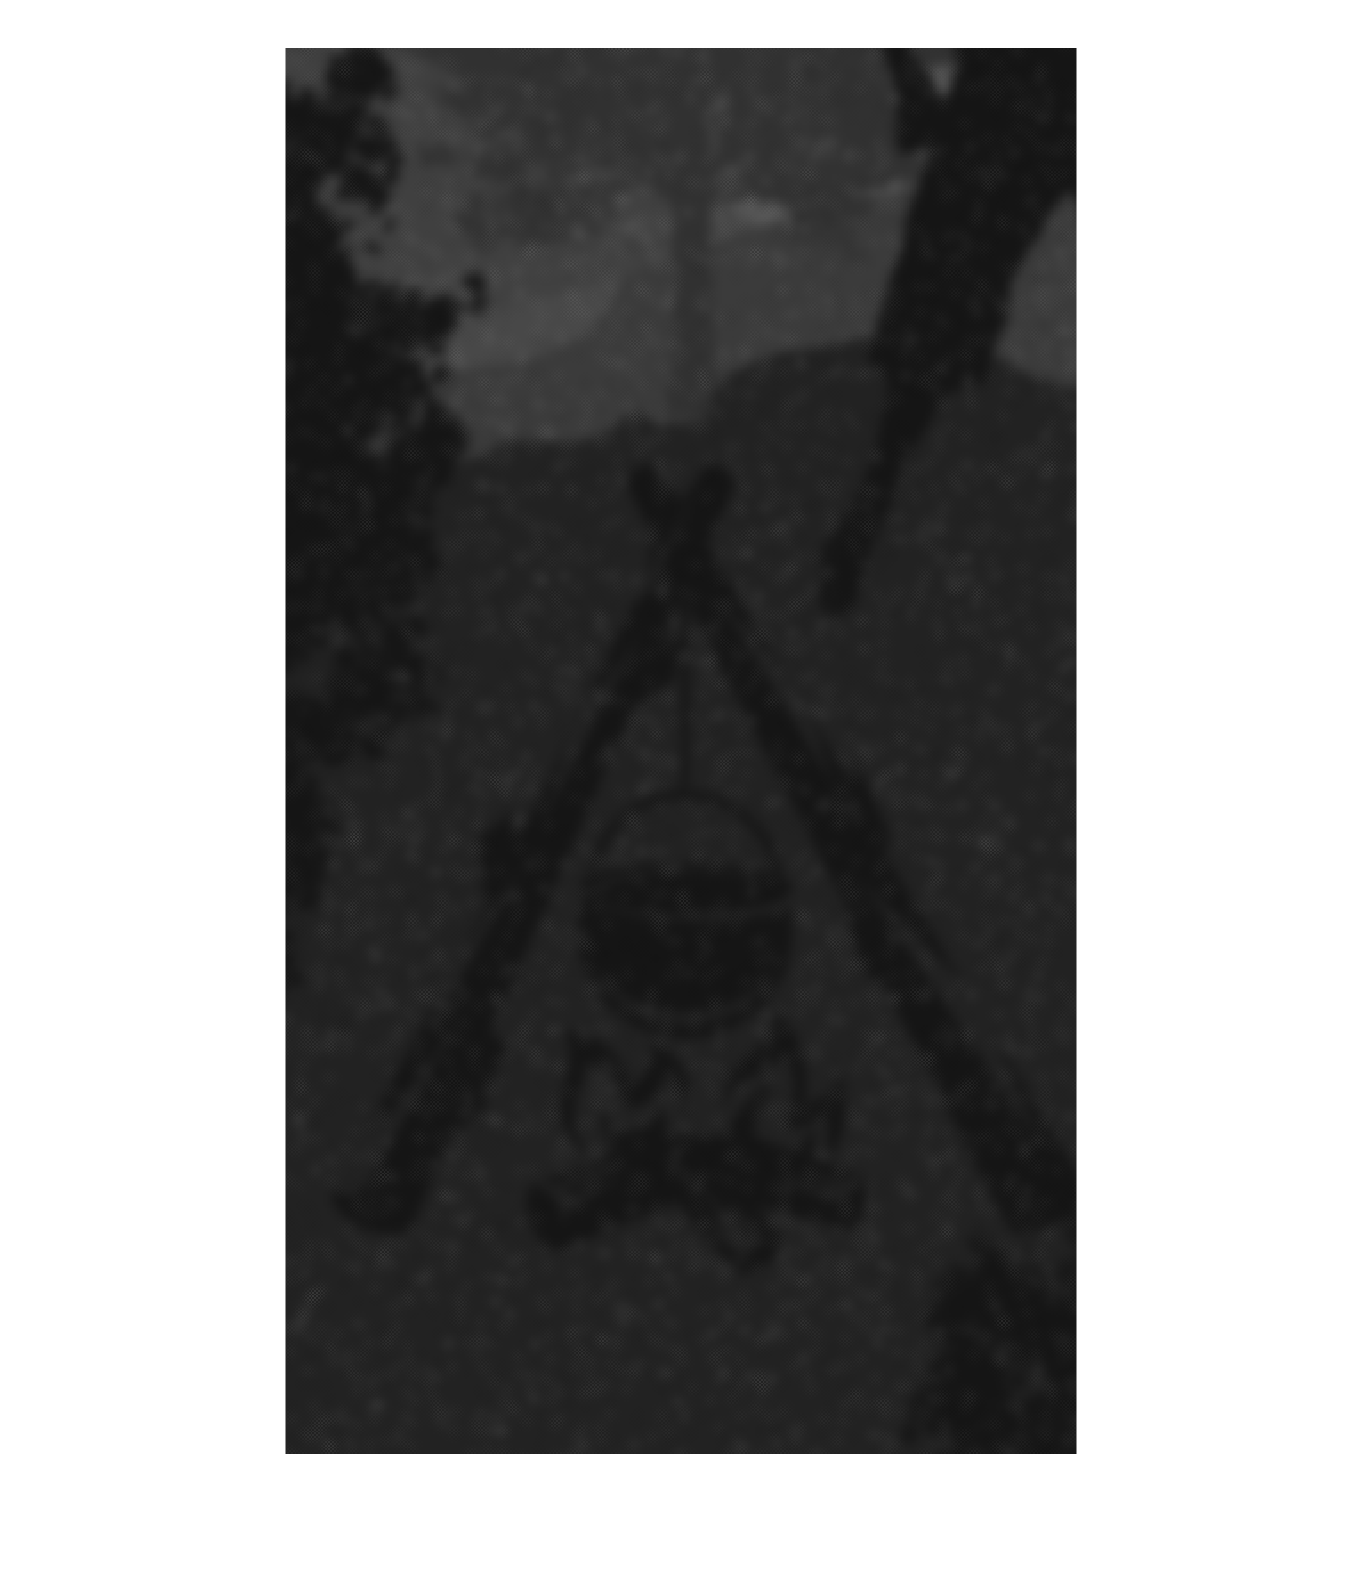
\includegraphics[scale=0.15]{Pictures/Esempi di utilizzo/Esempio 3/Dettaglio_SfondoForesta_filtrata_deltat0_25.png}
\caption{In ordine: immagine filtrata con delta\_t=0.1, e con delta\_t=0.25.}\label{fig:figura}
\end{figure} 

Vediamo quindi che aumentando questo parametro abbiamo un'immagine più sfuocata. Bisogna però fare attenzione poiché un valore anche solo di poco più alto può portare ad effetti distruttivi sull'immagine. Poniamo ad esempio delta\_t=0.3.

\begin{figure}[htb] \centering
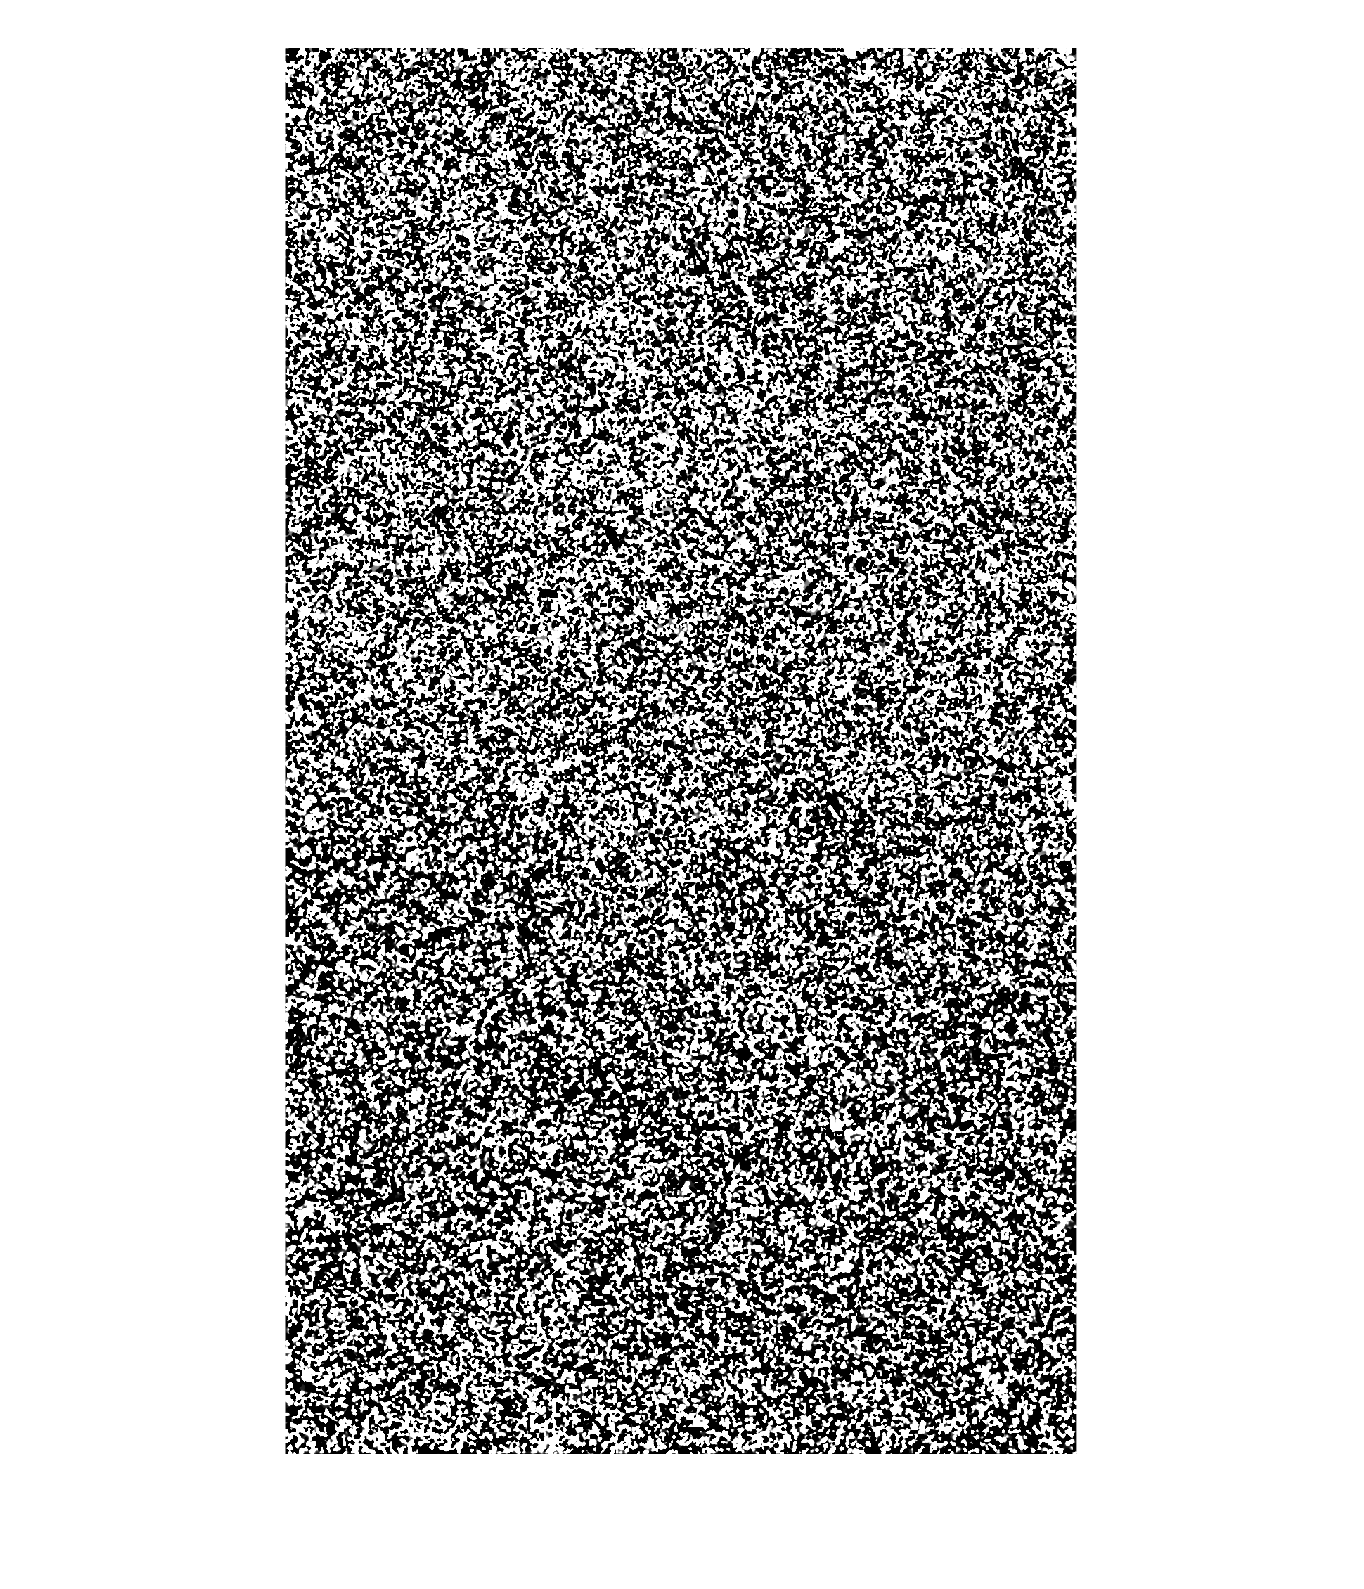
\includegraphics[scale=0.15]{Pictures/Esempi di utilizzo/Esempio 3/SfondoForesta_filtrata_deltat0_3.png}
\caption{Immagine filtrata con delta\_t=0.3.}\label{fig:figura}
\end{figure}
Questa evidenza sperimentale conferma quanto visto nell'\textbf{Osservazione 2.2.1}. Per garantire la stabilità numerica occorre quindi utilizzare valori $delta\_t \in [0,\frac{1}{4}]$.

\newpage
\subsection{Esempio 4 - Variazione della costante di controllo}
Adesso vediamo la costante c di controllo, la quale influenza il coefficiente c che è ciò che caratterizza il metodo differenziandolo dalla sola applicazione dell'equazione del calore. Vediamo come questo parametro regola in che misura i bordi verranno preservati e come cambiarla influisca con i risultati.\\
Parametri:
\begin{itemize}
    \item num\_iter=20
    \item delta\_t=0.1
    \item c=6, 20, 60
    \item sigma=1
\end{itemize}

\begin{figure}[htb] \centering
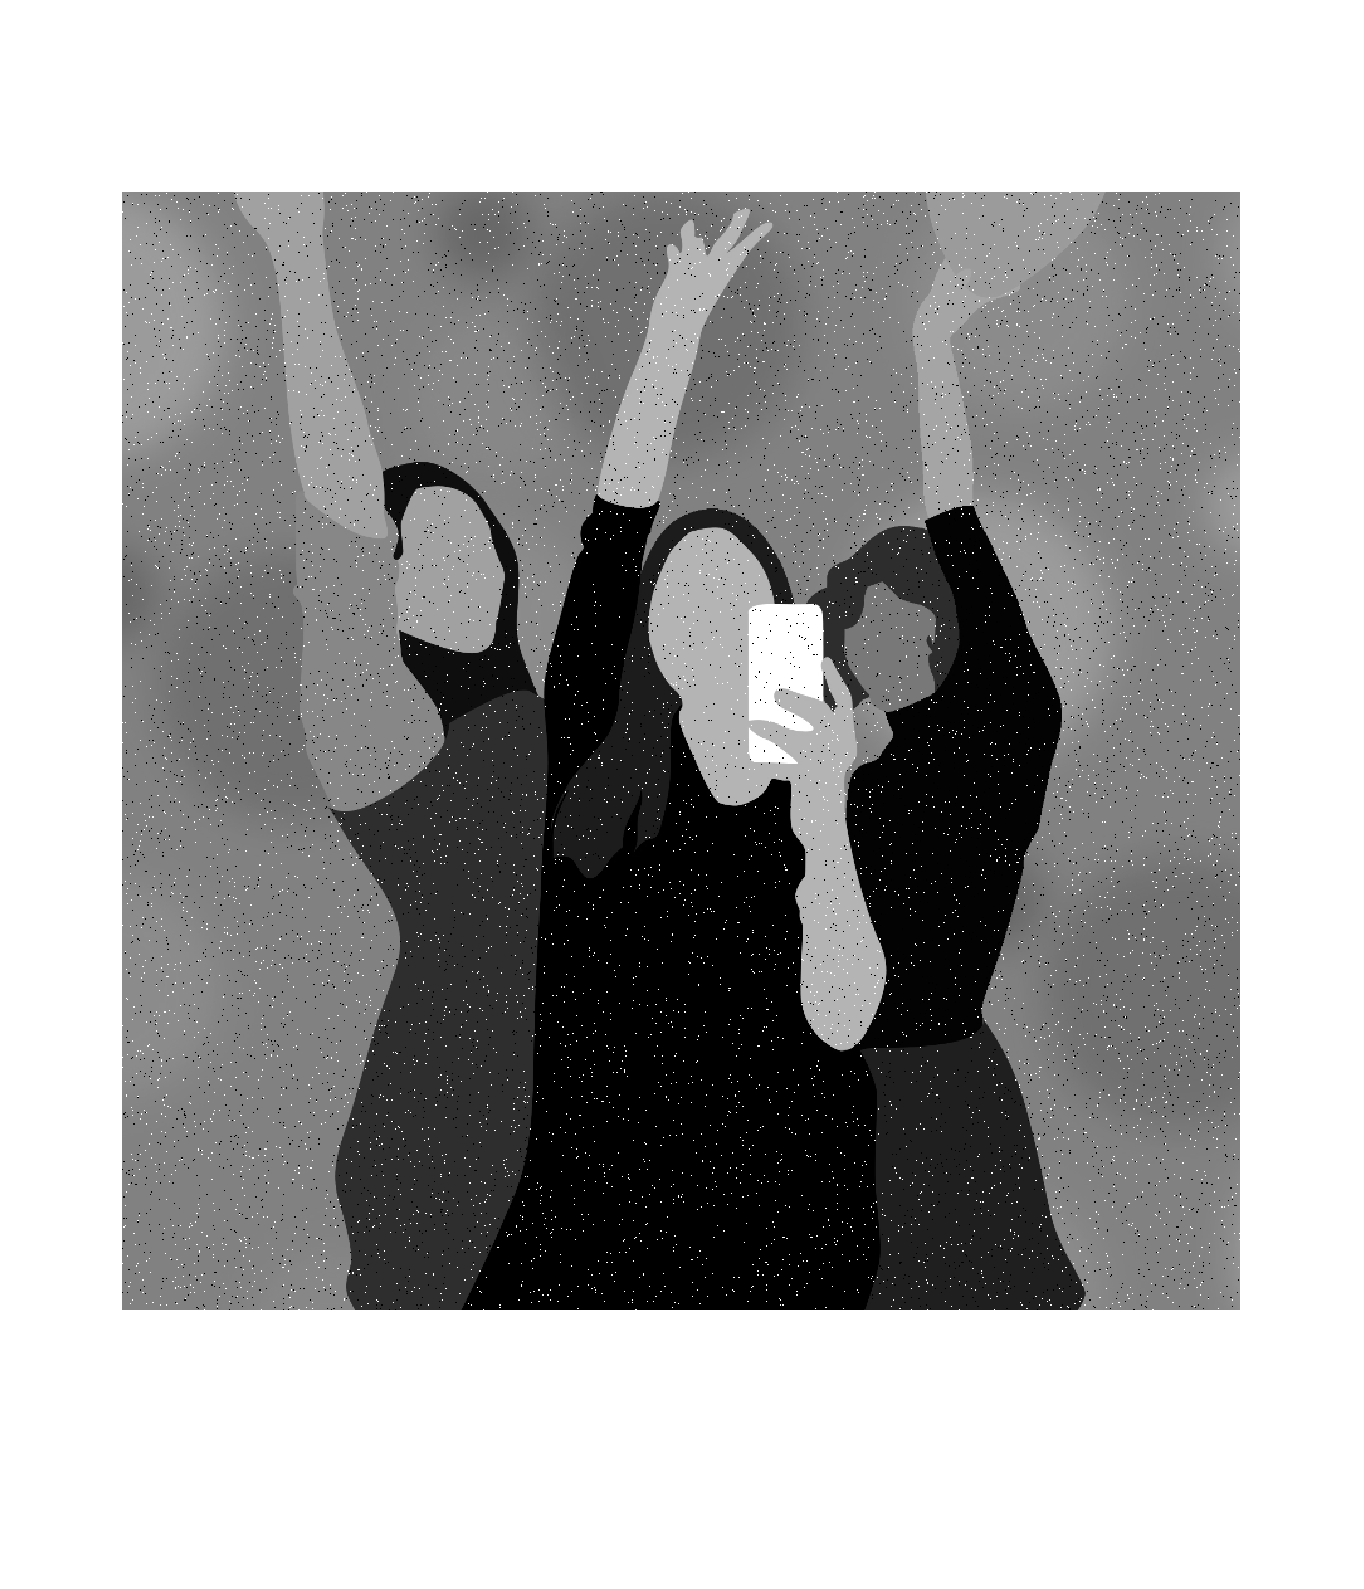
\includegraphics[scale=0.15,trim={0 3cm 0 5cm},clip]{Pictures/Esempi di utilizzo/Esempio 4/party_originale.png}
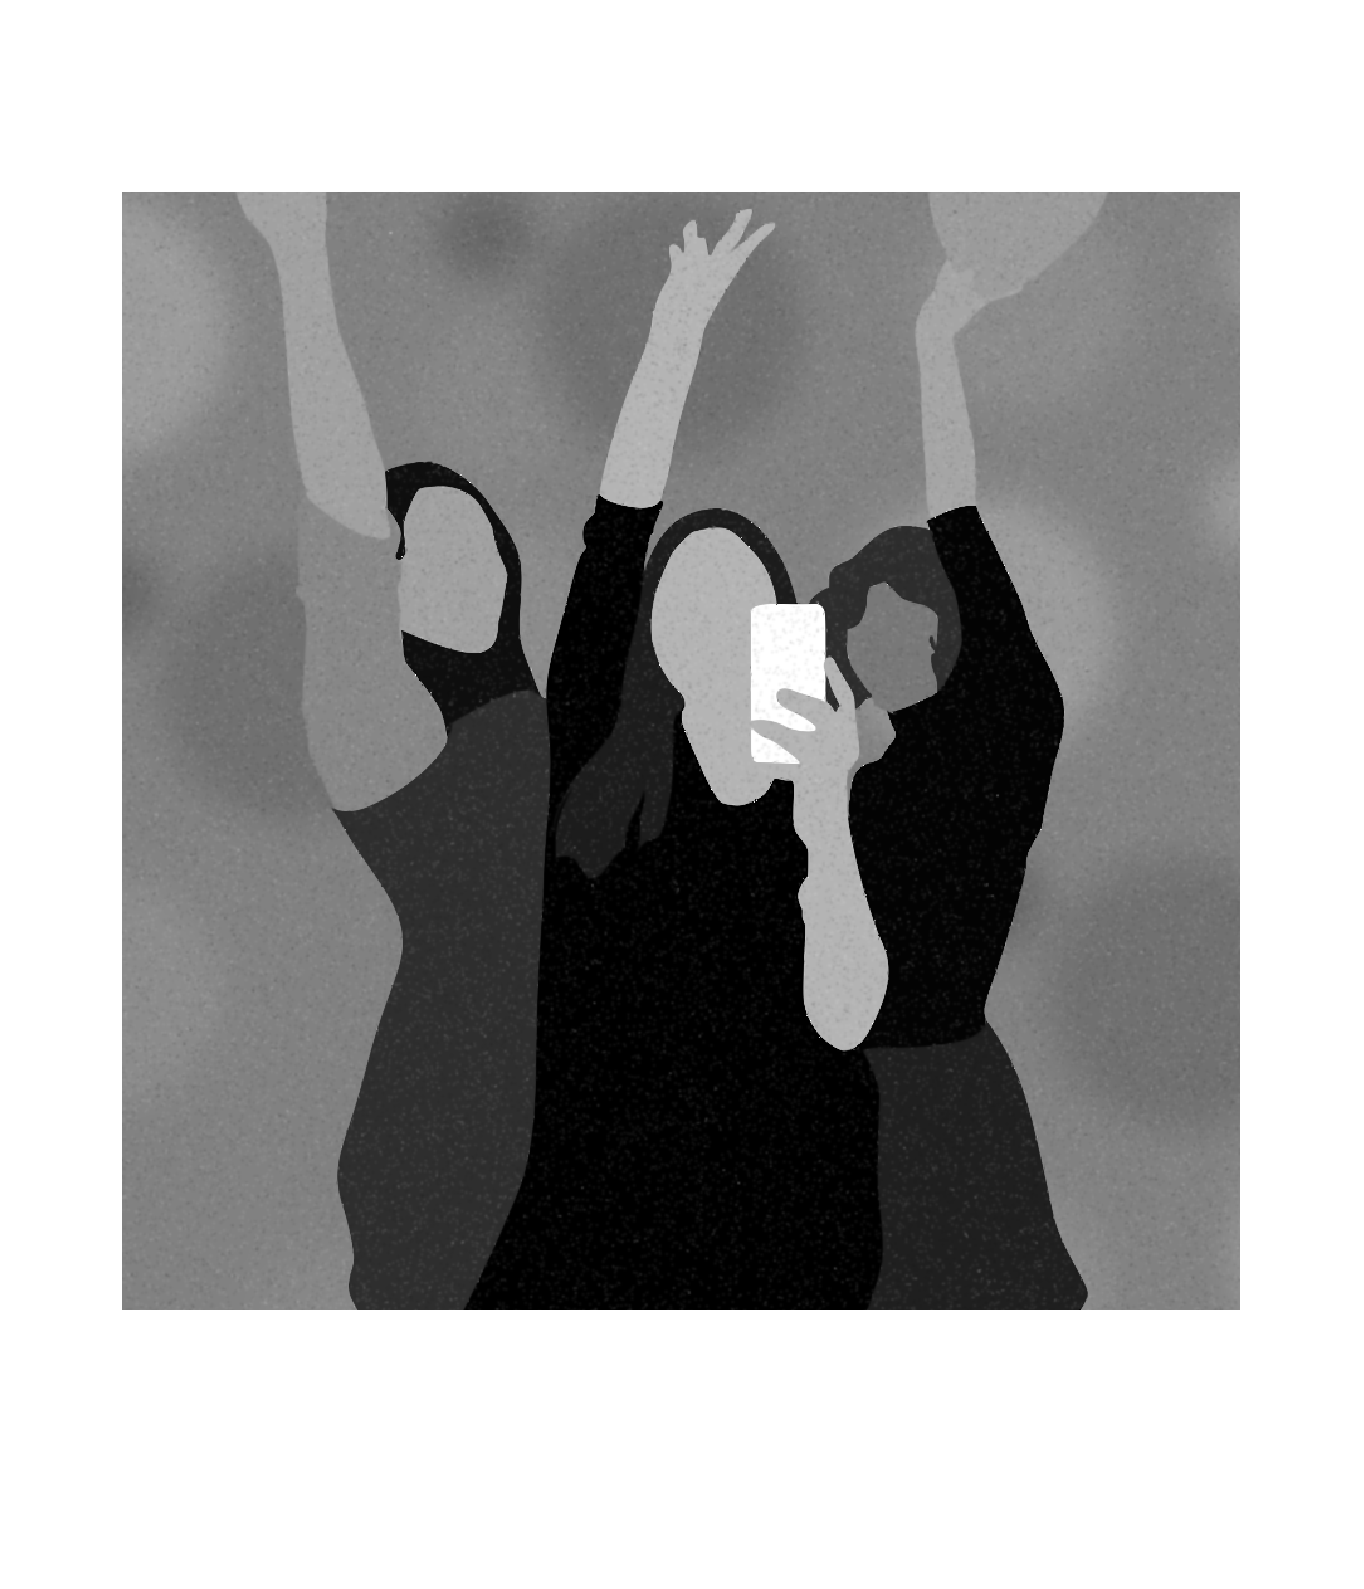
\includegraphics[scale=0.15,trim={0 3cm 0 5cm},clip]{Pictures/Esempi di utilizzo/Esempio 4/party_filtrata_kappa6.png}
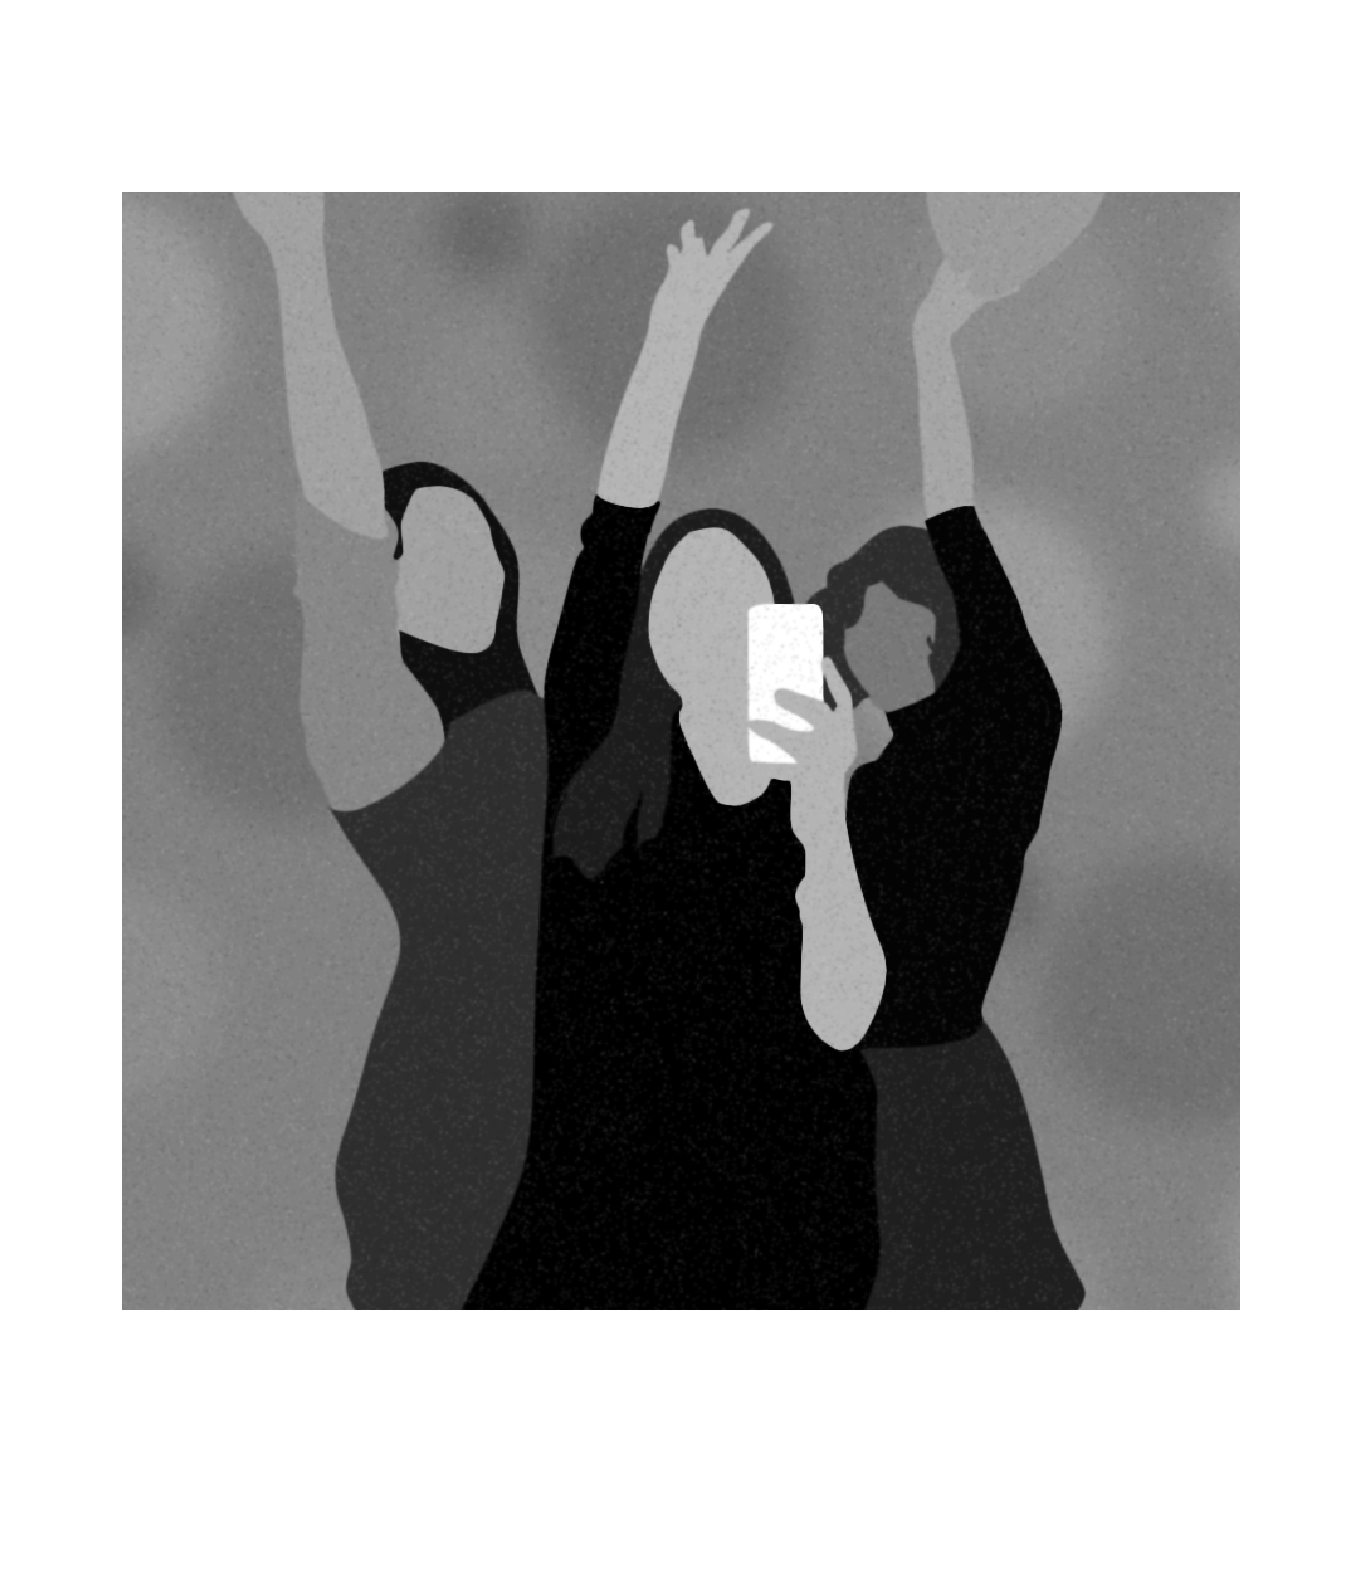
\includegraphics[scale=0.15,trim={0 5cm 0 3cm},clip]{Pictures/Esempi di utilizzo/Esempio 4/party_filtrata_kappa20.png}
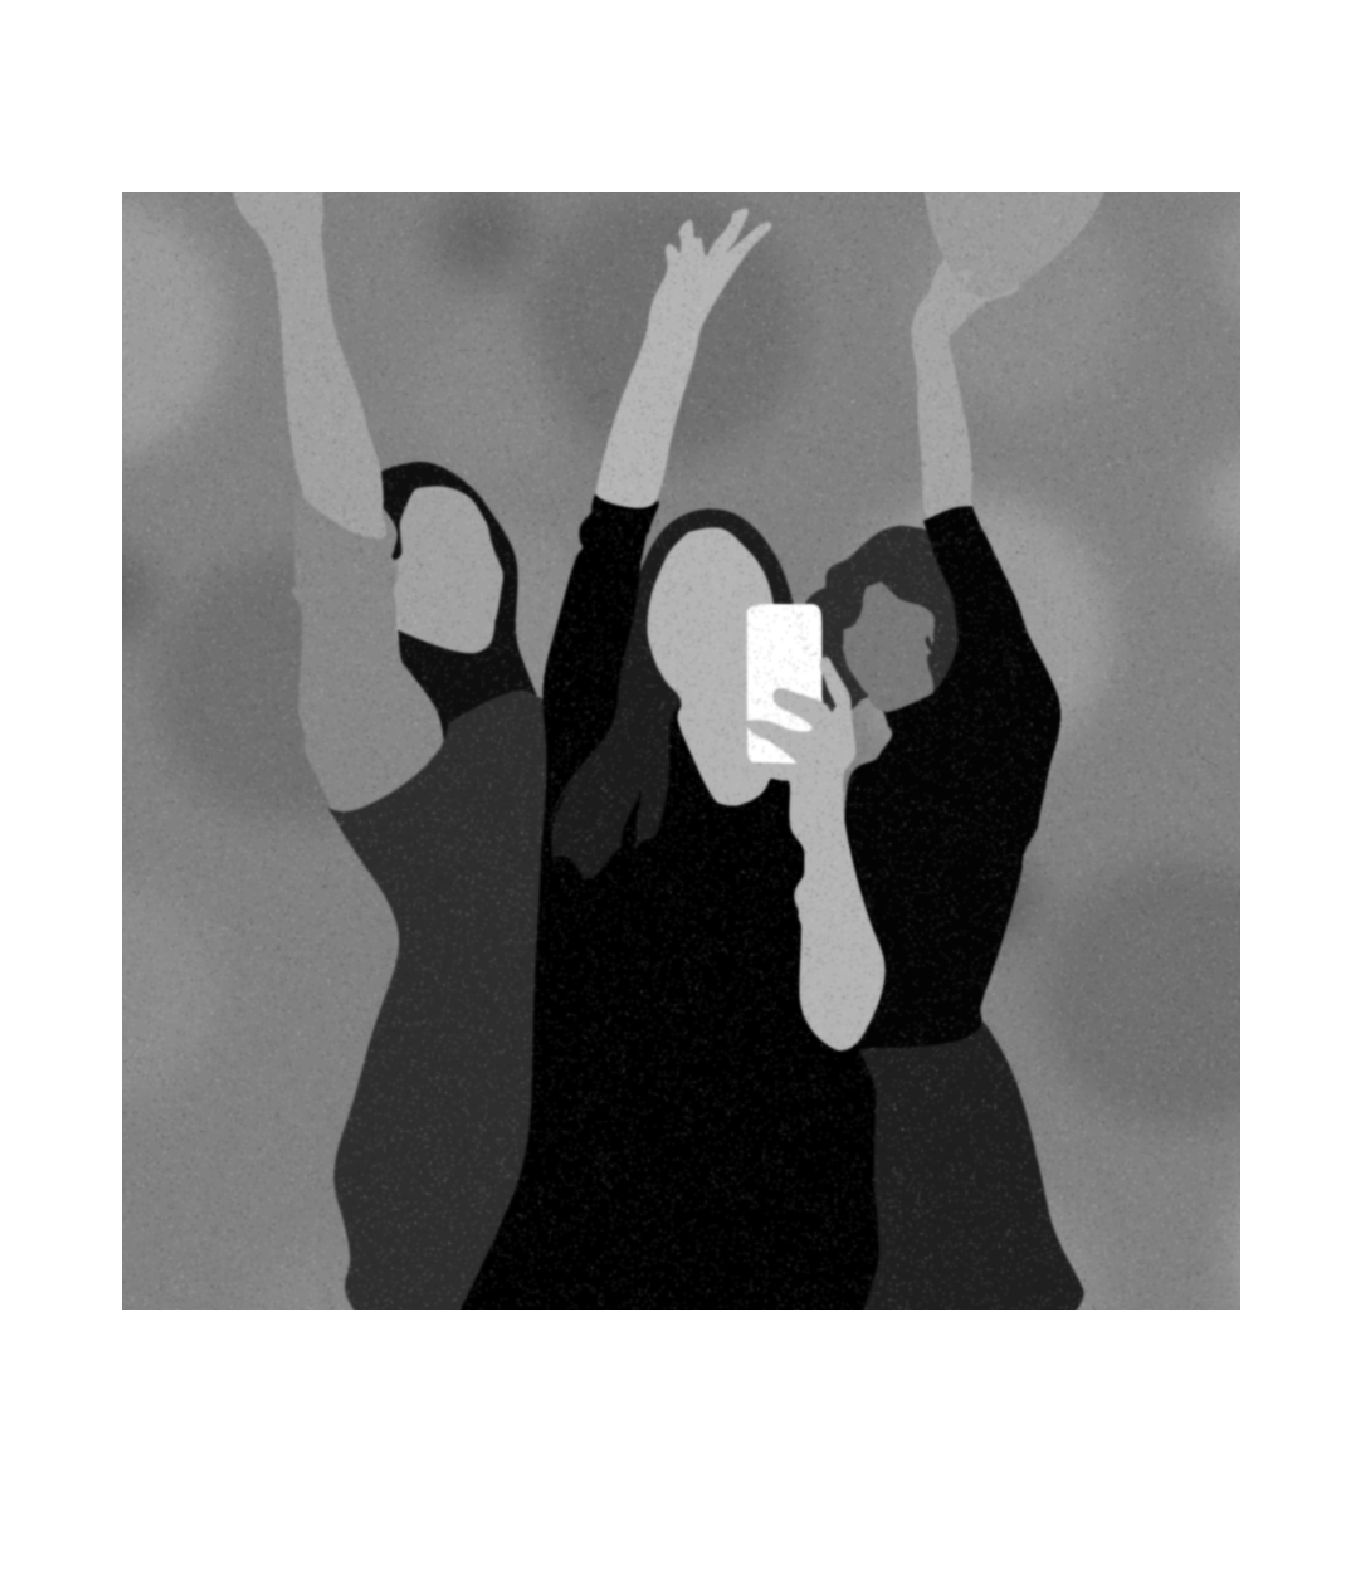
\includegraphics[scale=0.15,trim={0 5cm 0 3cm},clip]{Pictures/Esempi di utilizzo/Esempio 4/party_filtrata_kappa60.png}
\caption{In ordine: immagine con rumore, immagine filtrata con c=6, con c=20 e con c=60.}\label{fig:figura}
\end{figure} 
Questi esempi ci permettono di apprezzare come al crescere di c abbiamo una maggior riduzione del rumore, mentre i bordi vengono preservati meno.\\
Analiticamente $c=c(|\frac{\nabla(u)}{k}|^2)\Longrightarrow$ al crescere i bordi vengono preservati meno.\\

\newpage
\subsubsection{Casi limite: c alto}
\begin{itemize}
    \item num\_iter=20
    \item delta\_t=0.1
    \item c=60000
    \item sigma=1
\end{itemize}

\begin{figure}[htb] \centering
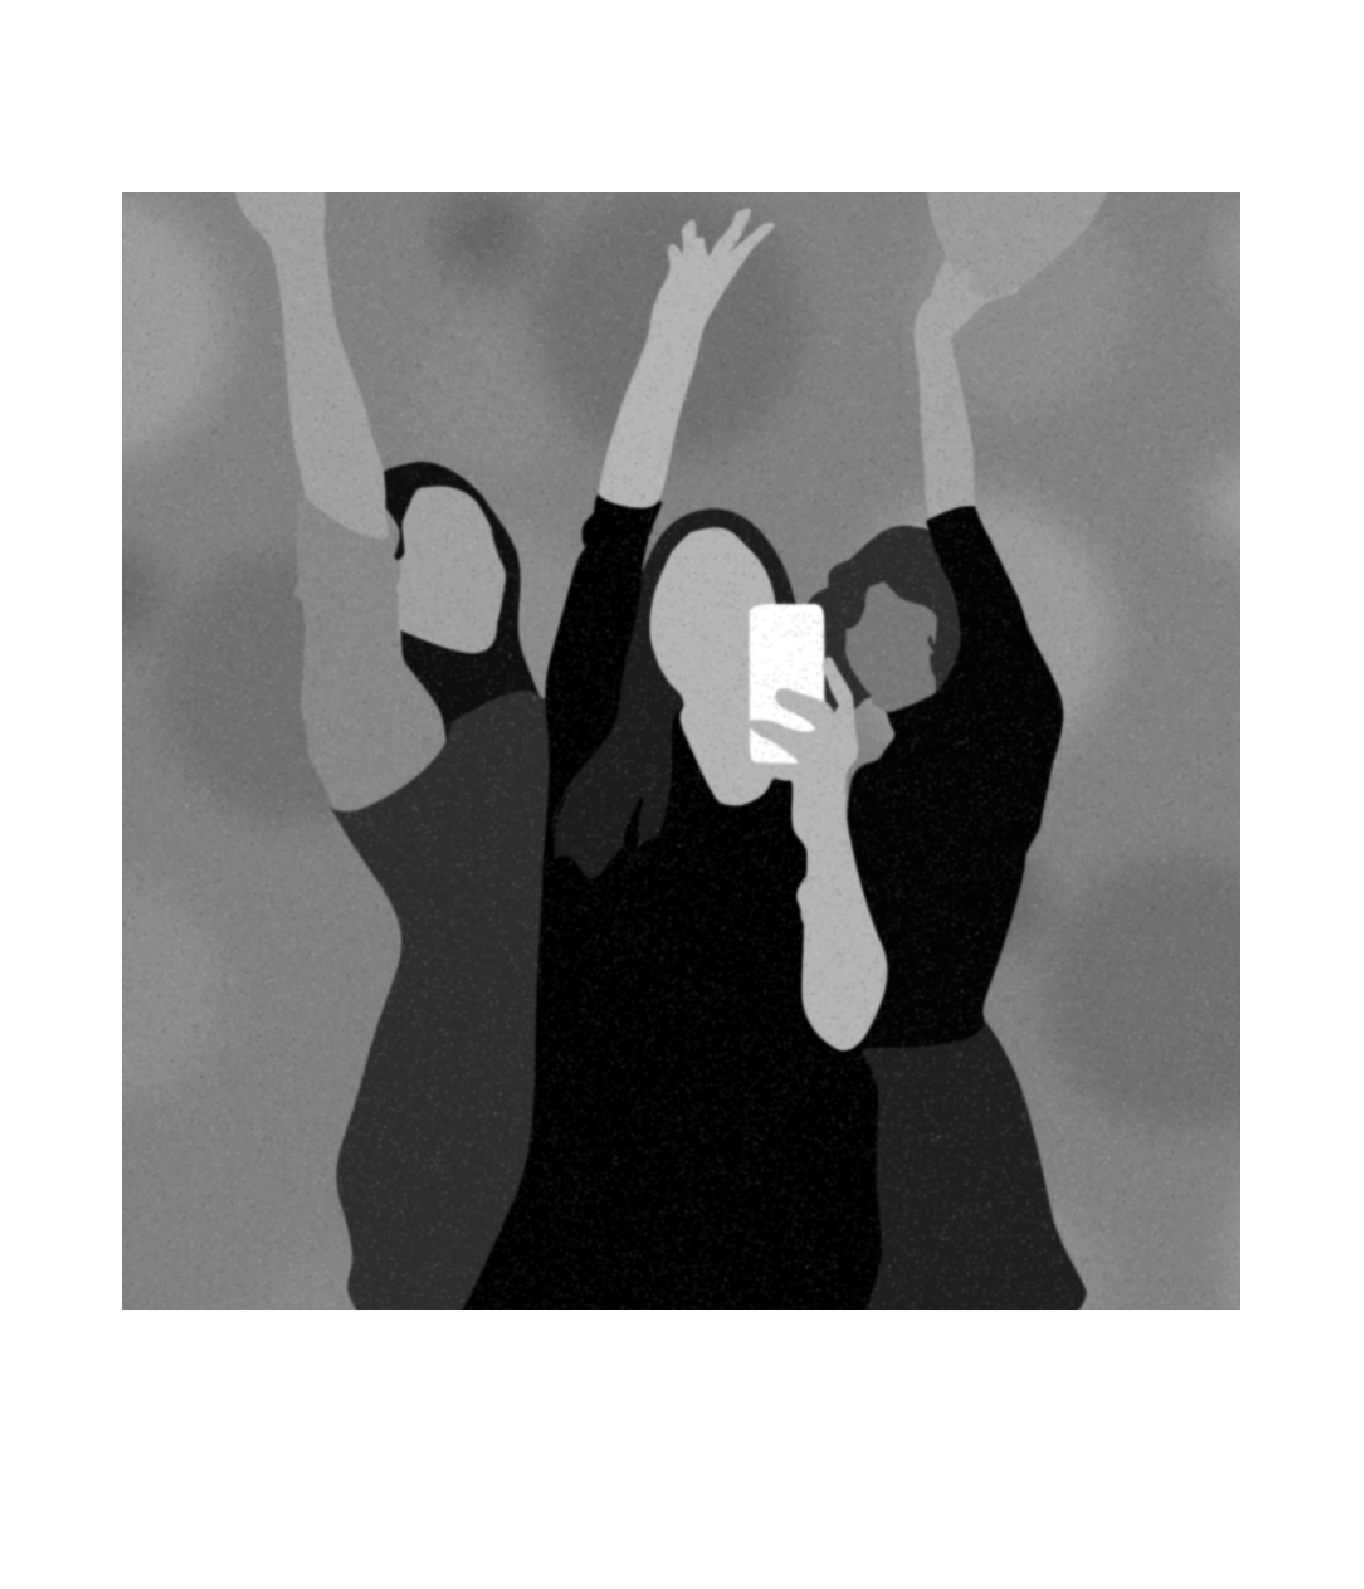
\includegraphics[scale=0.15,trim={0 3cm 0 5cm},clip]{Pictures/Esempi di utilizzo/Esempio 4/party_caso_limite_kappaalto.png}
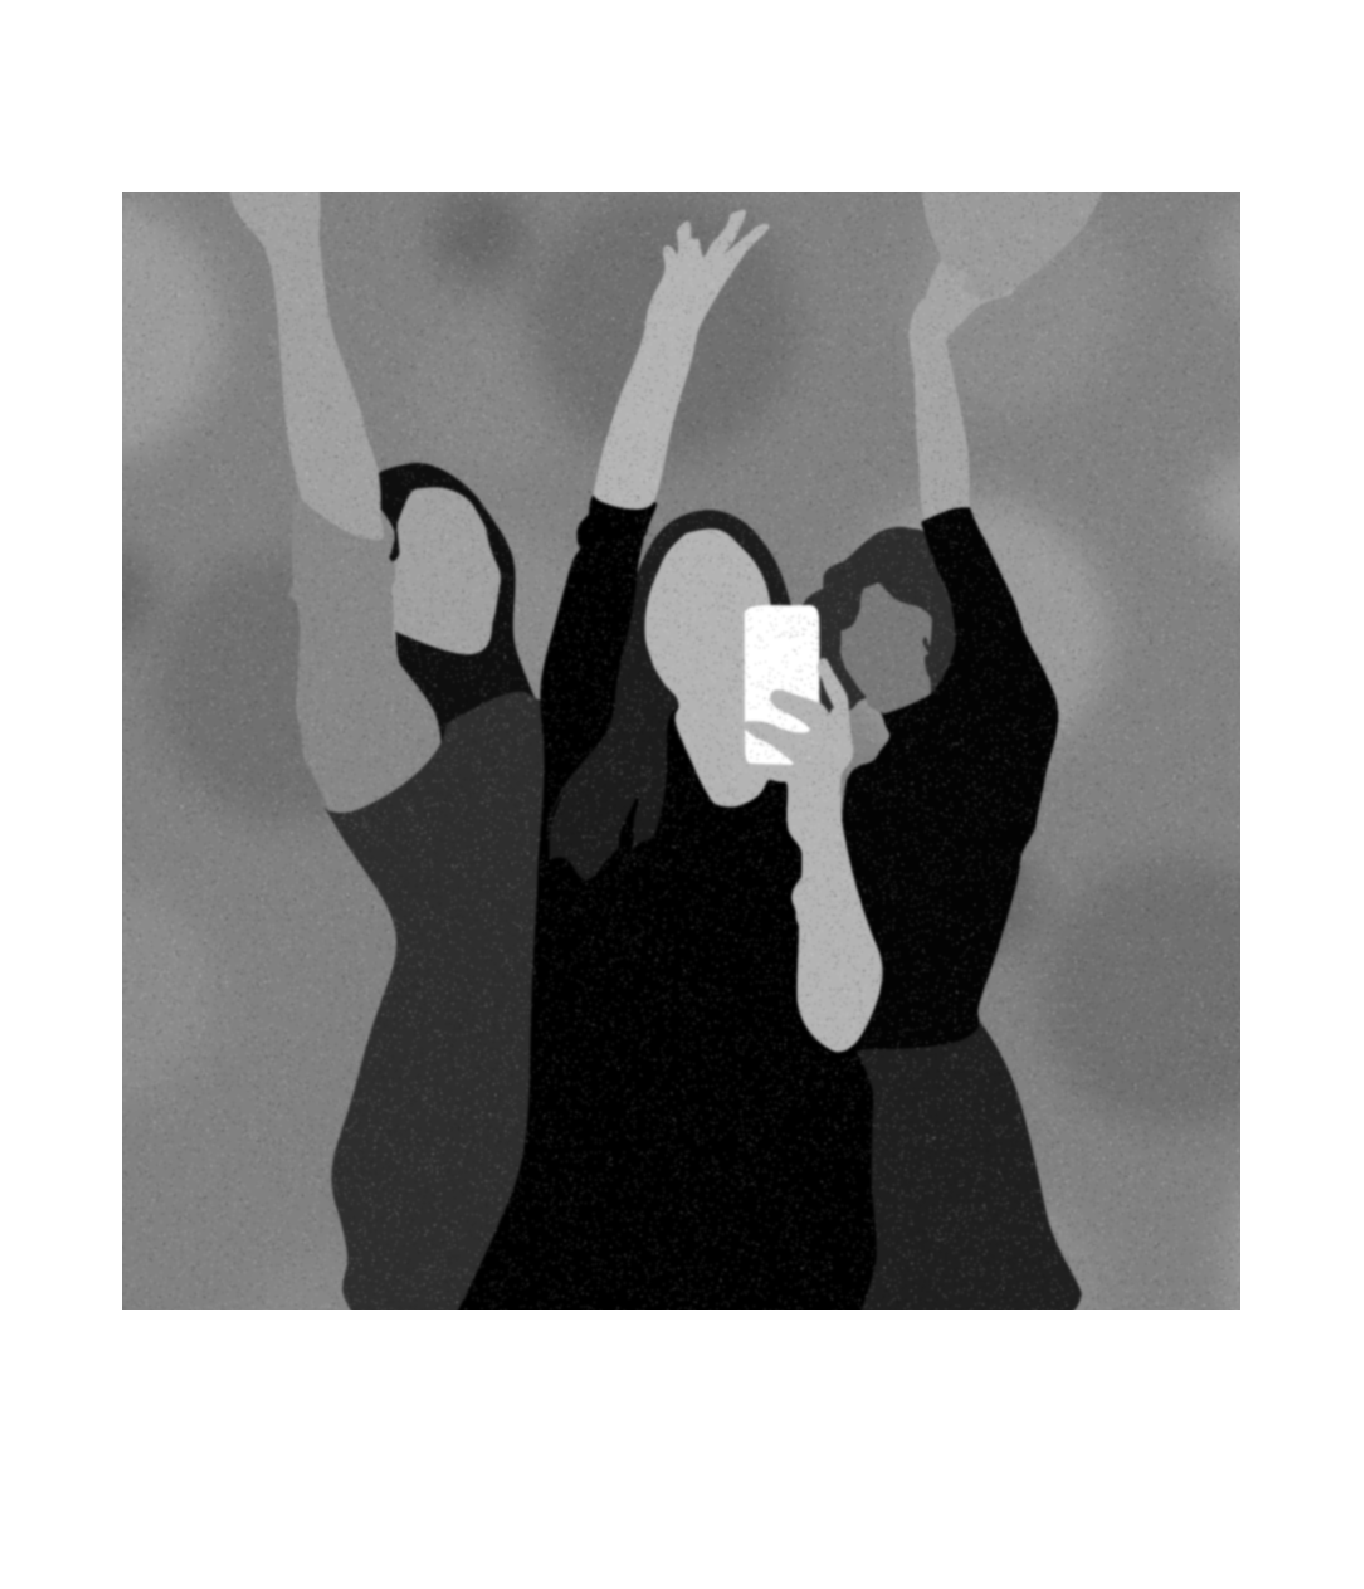
\includegraphics[scale=0.15,trim={0 3cm 0 5cm},clip]{Pictures/Esempi di utilizzo/Esempio 4/party_caso_limite_eq_calore.png}
\caption{In ordine: immagine filtrata con c=60000 e immagine filtrata con equazione del calore.}\label{fig:figura}
\end{figure} 
Analogamente, con un valore molto alto possiamo vedere che l'immagine sembra solamente diffusa, e infatti $c=c(|\frac{\nabla(u)}{k}|^2)\Longrightarrow\lim_{k\to\infty}c(|\frac{\nabla(u)}{k}|^2)=1$.\\
Ma allora $\frac{\partial u}{\partial t}(t,x)=div(c\nabla(u))=div(\nabla(u))=\Delta(u)$ ritrovando quindi l'equazione del calore, numericamente infatti troviamo:
\texttt{min(min([cN,cS,cW,cE]))=0.999996871393924} e \texttt{max(max([cN,cS,cW,cE]))=1}
riconosciamo quindi un appiattimento di c ad 1.

\newpage
\subsubsection{Casi limite: c basso}
Parametri:
\begin{itemize}
    \item num\_iter=20
    \item delta\_t=0.1
    \item c=0.001
    \item sigma=1
\end{itemize}

\begin{figure}[htb] \centering
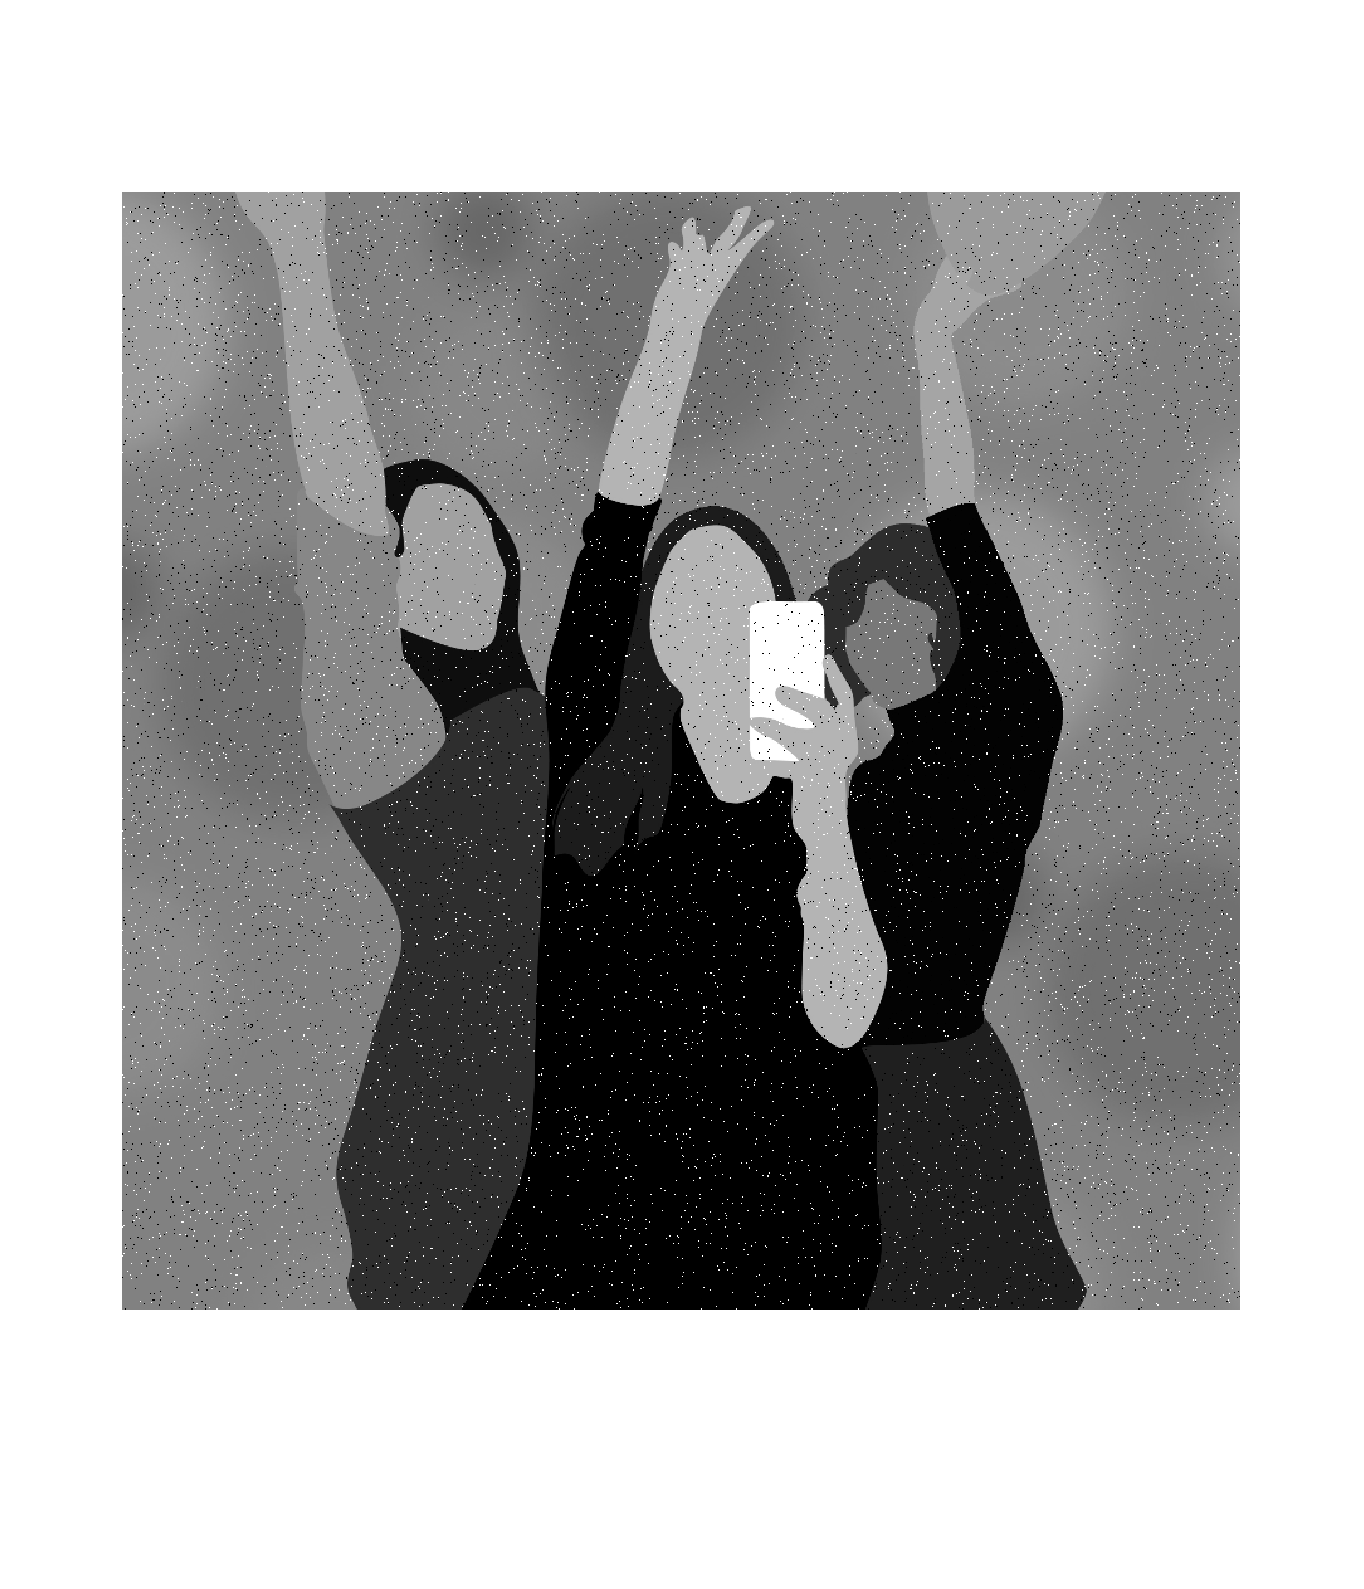
\includegraphics[scale=0.15,trim={0 3cm 0 5cm},clip]{Pictures/Esempi di utilizzo/Esempio 4/party_caso_limite_originale.png}
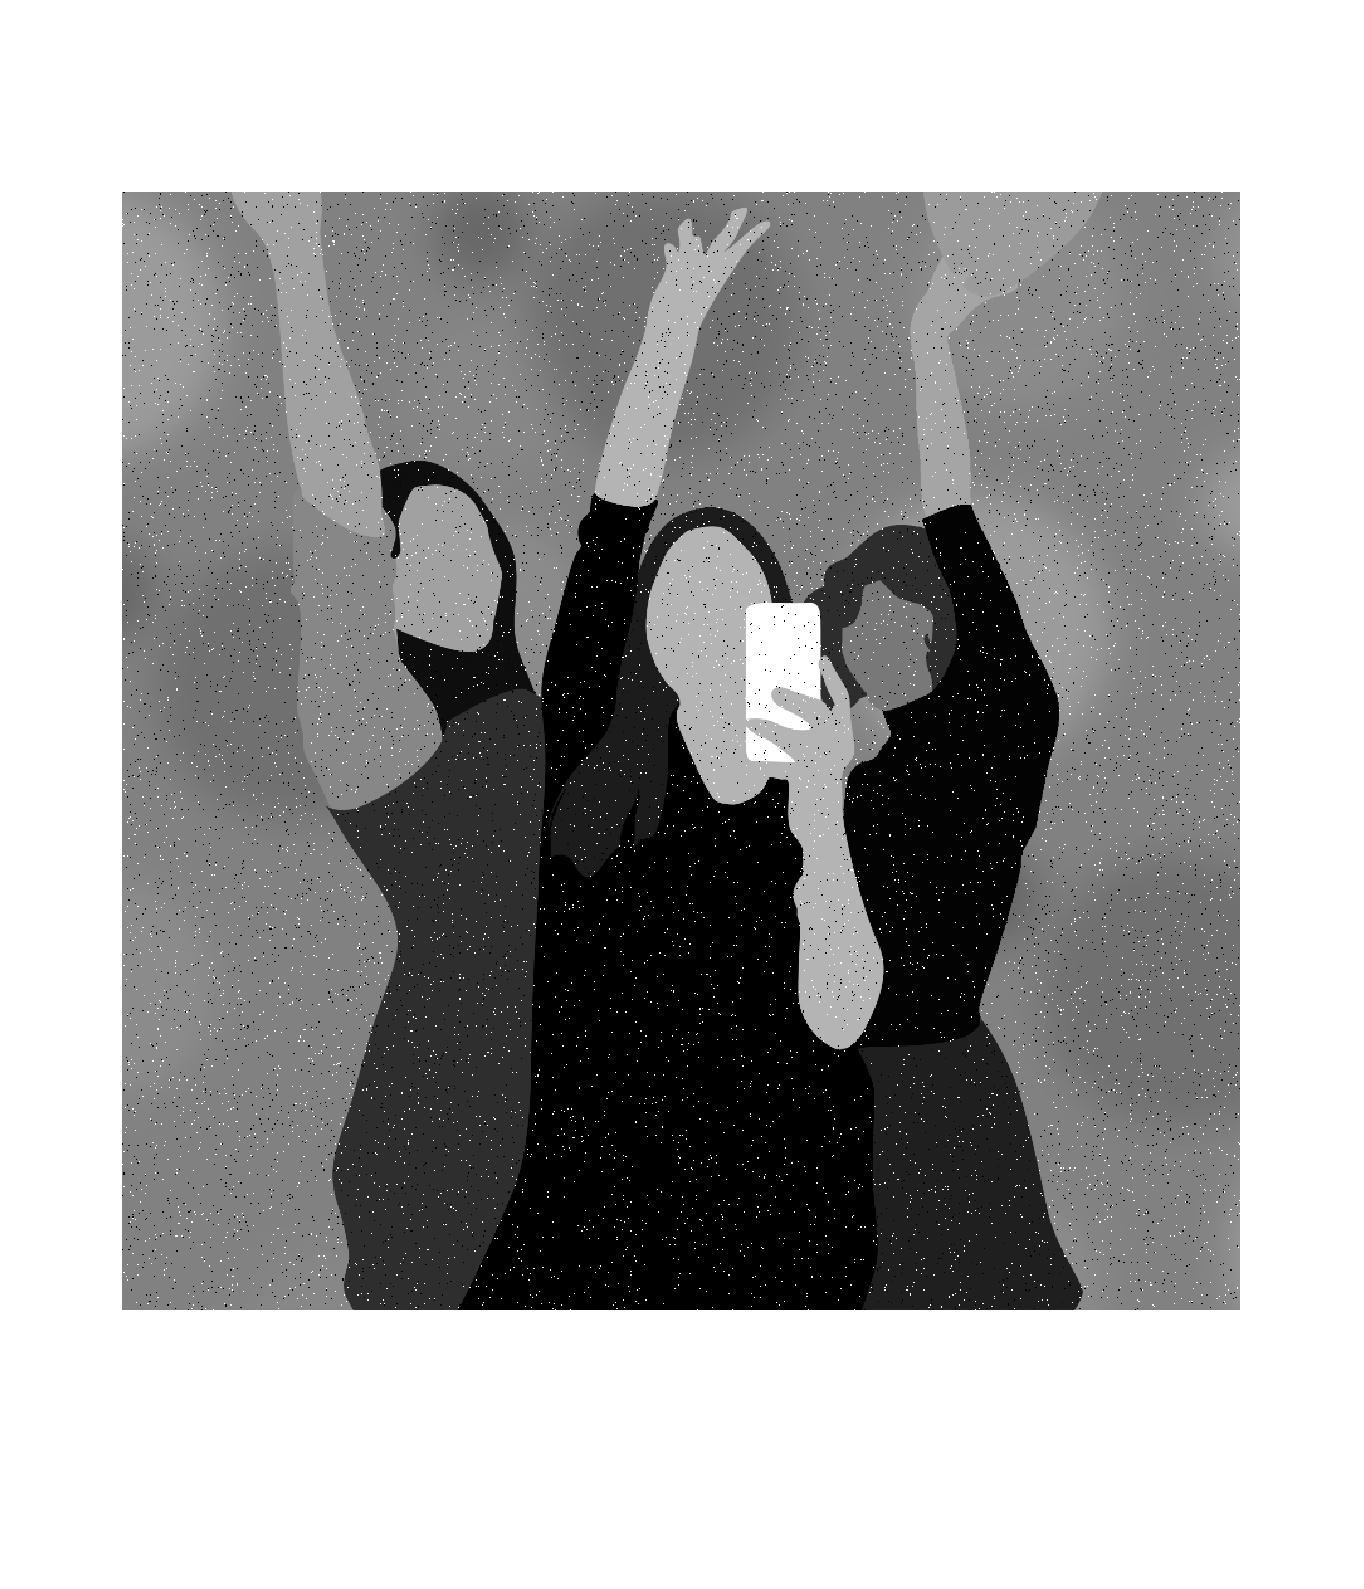
\includegraphics[scale=0.15,trim={0 3cm 0 5cm},clip]{Pictures/Esempi di utilizzo/Esempio 4/party_caso_limite_kappabasso.png}
\caption{In ordine: immagine con rumore e immagine filtrata con c=0.001.}\label{fig:figura}
\end{figure} 
Possiamo facilmente notare come con un valore molto basso di c l'immagine sembra non subire variazioni, effettivamente
$c=c(|\frac{\nabla(u)}{k}|^2)\Longrightarrow\lim_{k\to0}c(|\frac{\nabla(u)}{k}|^2)=0$.\\
Ma allora $\frac{\partial u}{\partial t}(t,x)=div(c\nabla(u))=div(0*\nabla(u))=0$, ma $\frac{\partial u}{\partial t}(t,x)=0 \Leftrightarrow u=cost$ cioè non c'è variazione.\\
In questo caso non riportiamo i dati sul massimo e sul minimo di c perché anche se ci aspettiamo un appiattimento sullo 0 ci sarà sicuramente qualche punto in cui non c'è variazione di colore la derivata sarà quindi nulla e per quanto piccolo possiamo scegliere k il rapporto farà comunque 0 e quindi c sarà 1. Questo non ci preoccupa siccome il metodo sfocherà una porzione d'immagine di colore costante per cui anche in questi punti non avremo nessuna variazione

\newpage
\subsection{Esempio 5  - Variazione della costante di diffusione}
Adesso vediamo la costante Sigma, la quale regola l'applicazione dell'equazione del calore che influenza il coefficiente c. Vediamo quindi anche in questo caso come questo parametro regola in che misura i bordi verranno preservati e come cambiarla influisca con i risultati.\\
Parametri:
\begin{itemize}
    \item num\_iter=20
    \item delta\_t=0.1
    \item c=60
    \item sigma=0.5, 1, 2
\end{itemize}

\begin{figure}[htb] \centering
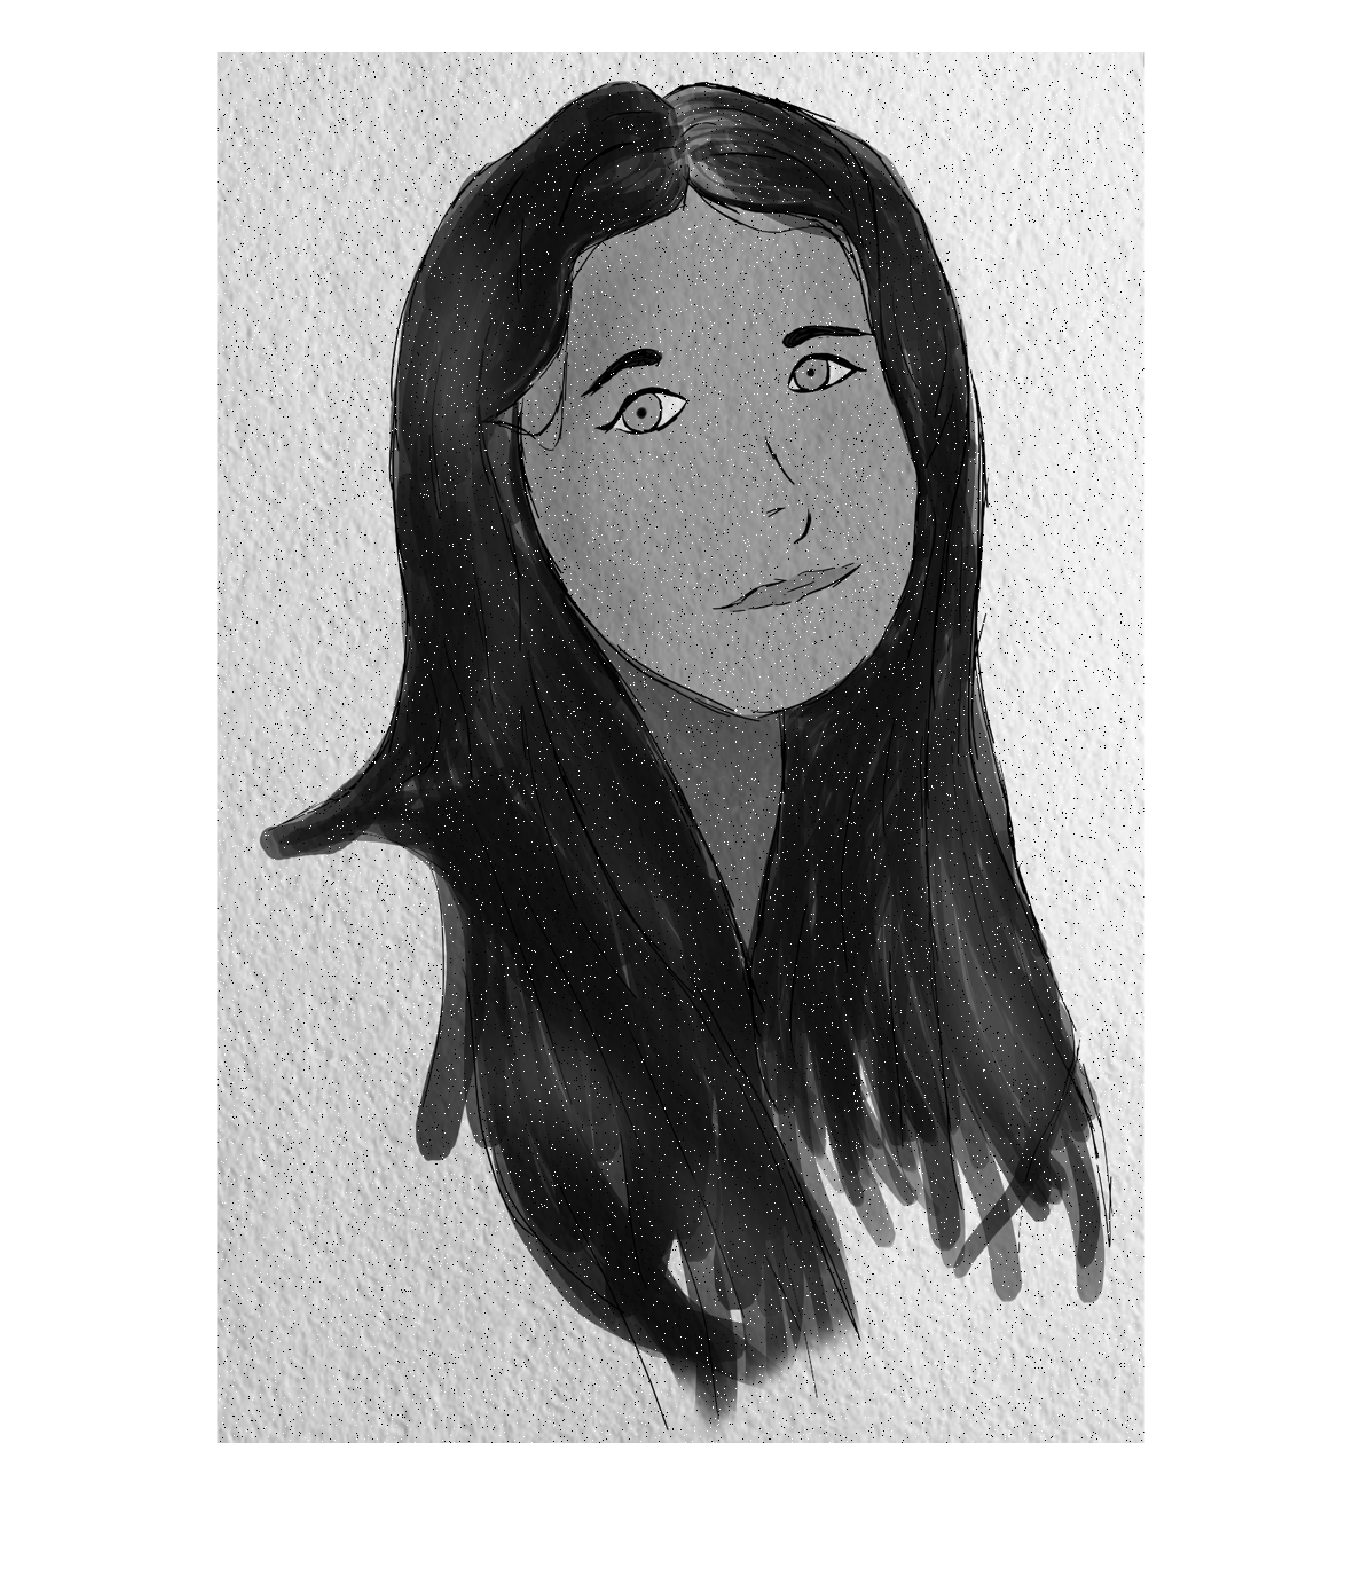
\includegraphics[scale=0.15,trim={0cm 3cm 3cm 0cm},clip]{Pictures/Esempi di utilizzo/Esempio 5/ami_originale_resize.png}
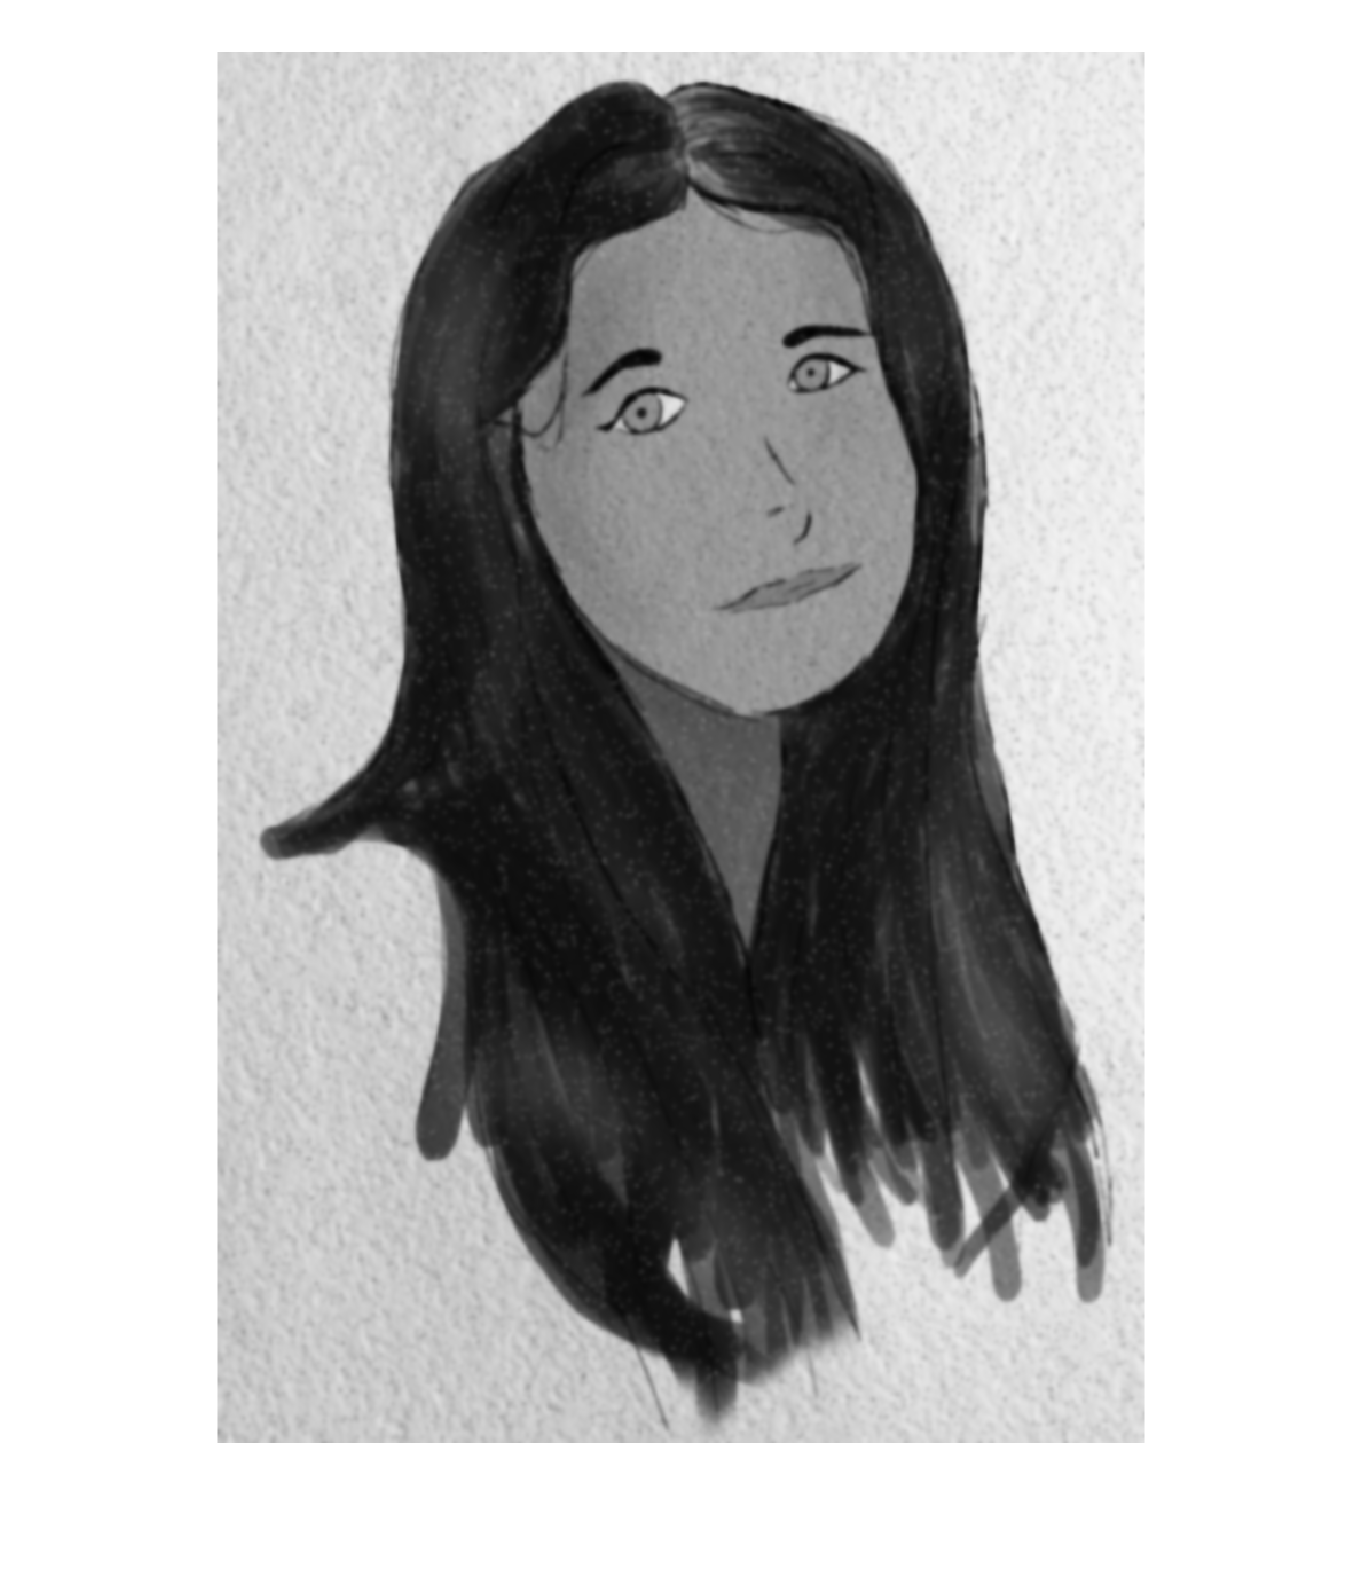
\includegraphics[scale=0.15,trim={3cm 3cm 0cm 0cm},clip]{Pictures/Esempi di utilizzo/Esempio 5/ami_filtrata_sigma0_5_kappa60_resize.png}
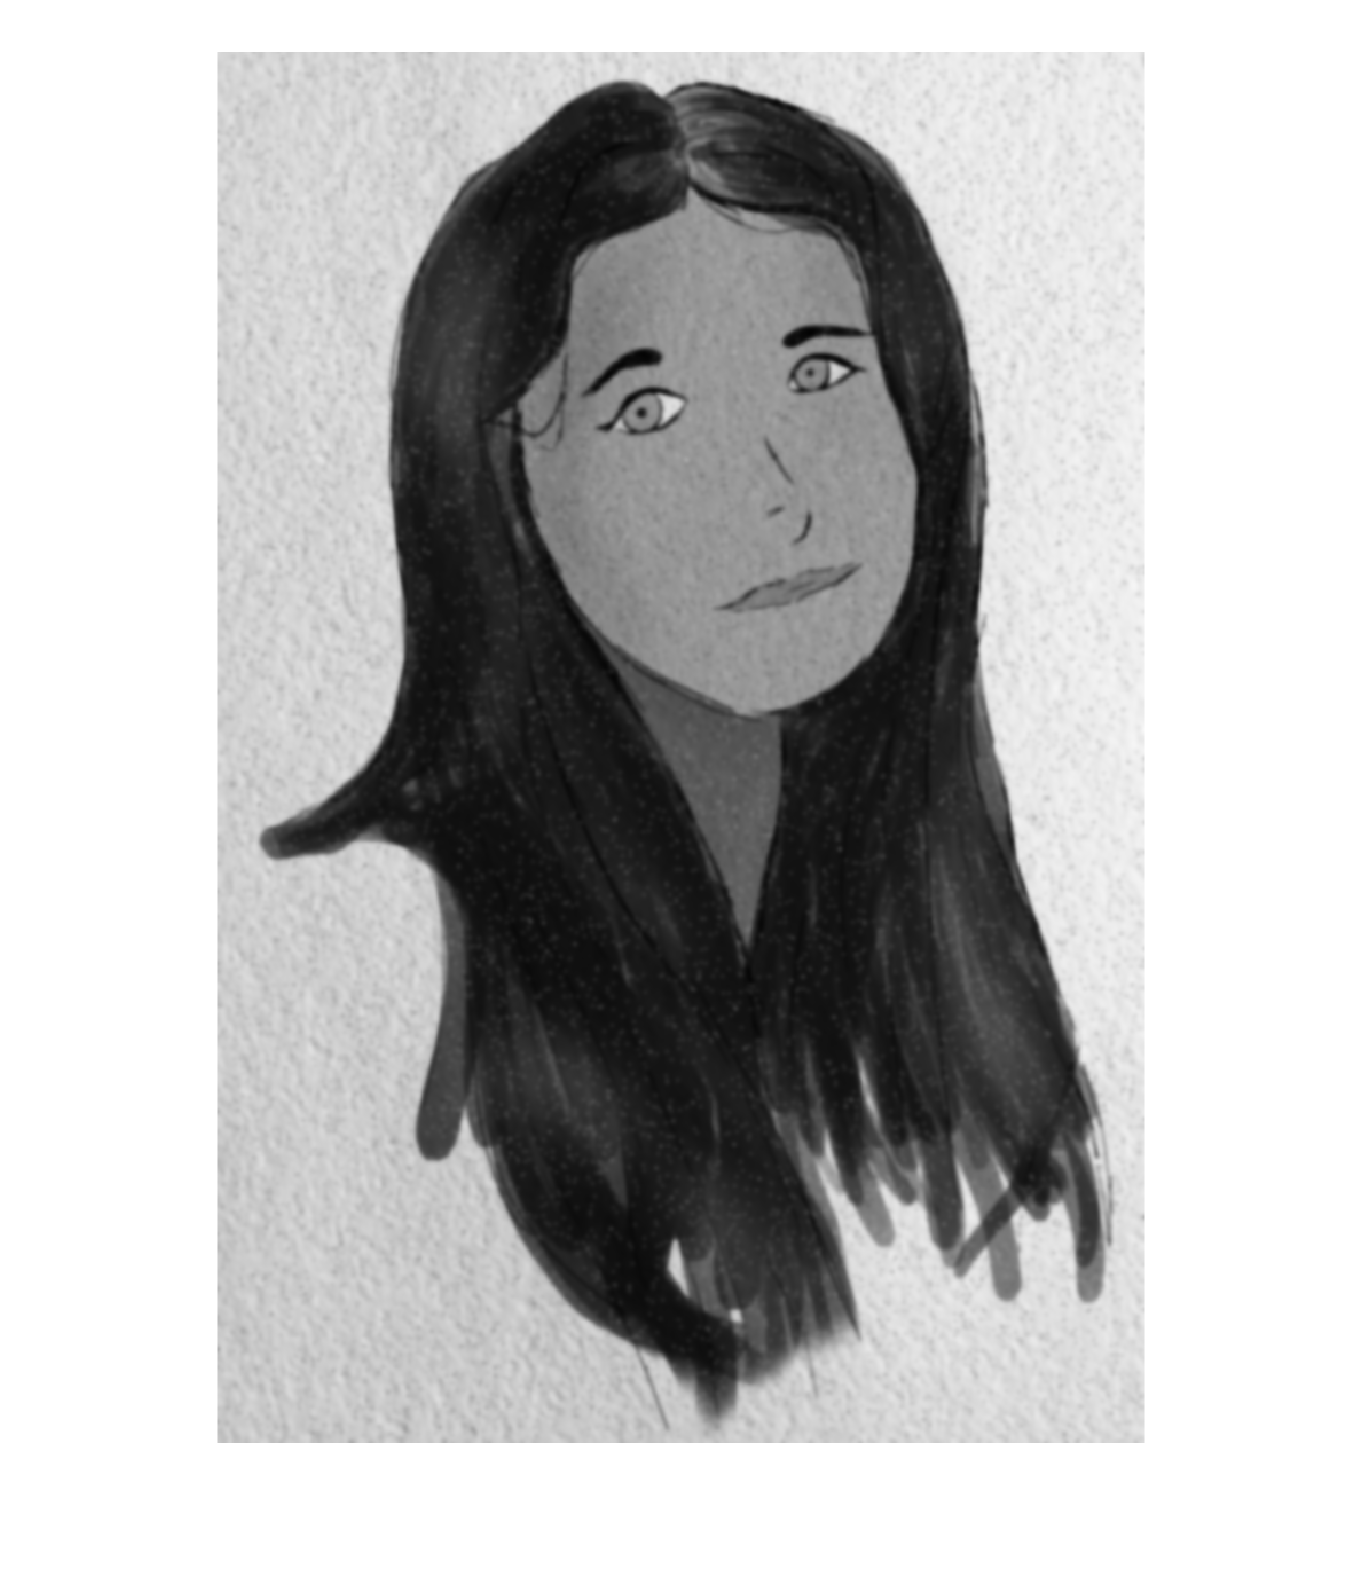
\includegraphics[scale=0.15,trim={0cm 0cm 3cm 0cm},clip]{Pictures/Esempi di utilizzo/Esempio 5/ami_filtrata_sigma1_kappa60_resize.png}
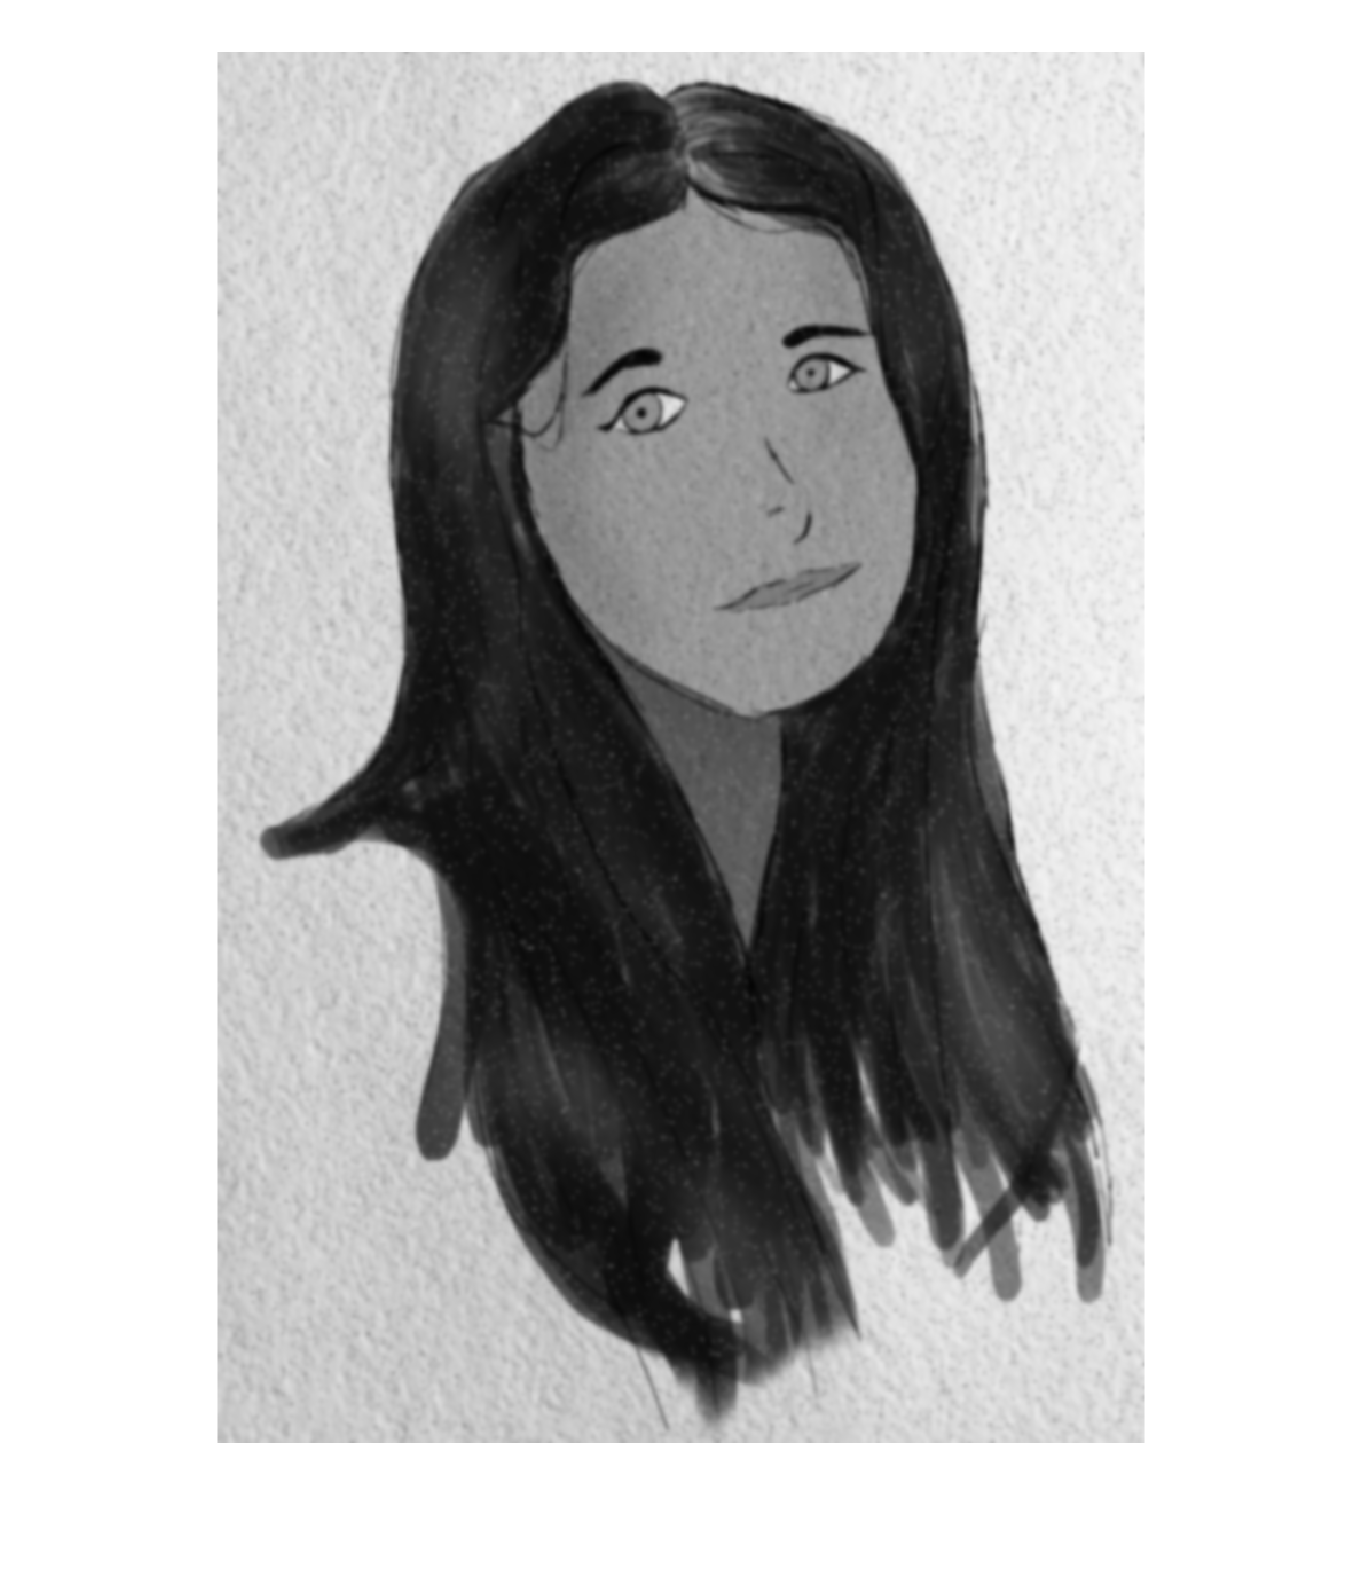
\includegraphics[scale=0.15,trim={3cm 0cm 0cm 0cm},clip]{Pictures/Esempi di utilizzo/Esempio 5/ami_filtrata_sigma2_kappa60_resize.png}
\caption{In ordine: immagine con rumore, immagine filtrata con sigma=0.5, con sigma=1 e con sigma=2.}\label{fig:figura}
\end{figure} 
Questi esempi però non ci permettono di apprezzare una gran differenza, infatti sigma influenza il gradiente, questo va però diviso per c che in questo caso è 60 appiattendo i valori del gradiente.\\
Infatti, $\frac{\nabla(u)_1}{k}-\frac{\nabla(u)_2}{k}=\frac{\nabla(u)_1-\nabla(u)_2}{k}$ cioè anche la differenza tra i due gradienti sarà 60 volte minore e quindi poco visibile.\\
Per rendere più evidenti queste differenze possiamo allora abbassare il valore di k.\\
Parametri:
\begin{itemize}
    \item num\_iter=20
    \item delta\_t=0.1
    \item c=0.5
    \item sigma=0.5, 1, 2
\end{itemize}

\begin{figure}[htb] \centering
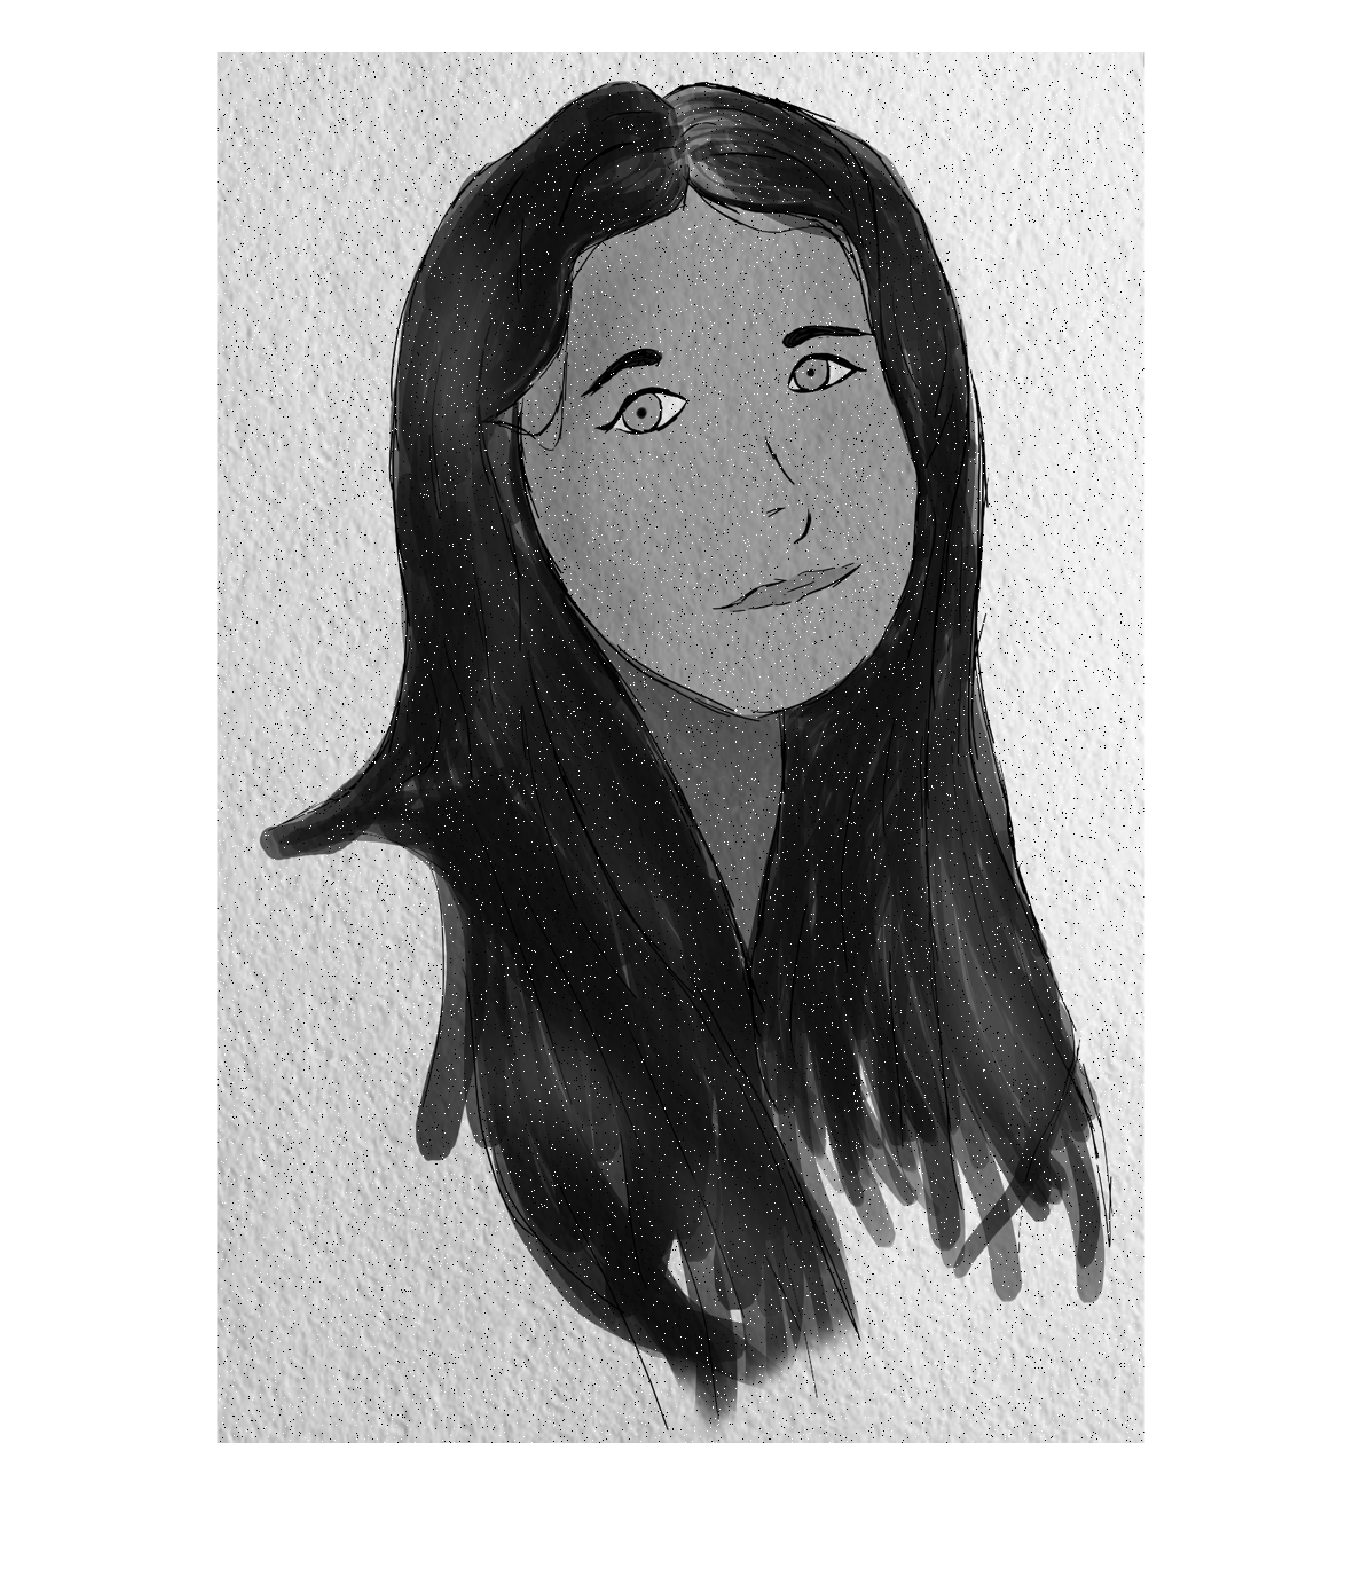
\includegraphics[scale=0.15,trim={0cm 3cm 3cm 0cm},clip]{Pictures/Esempi di utilizzo/Esempio 5/ami_originale_resize.png}
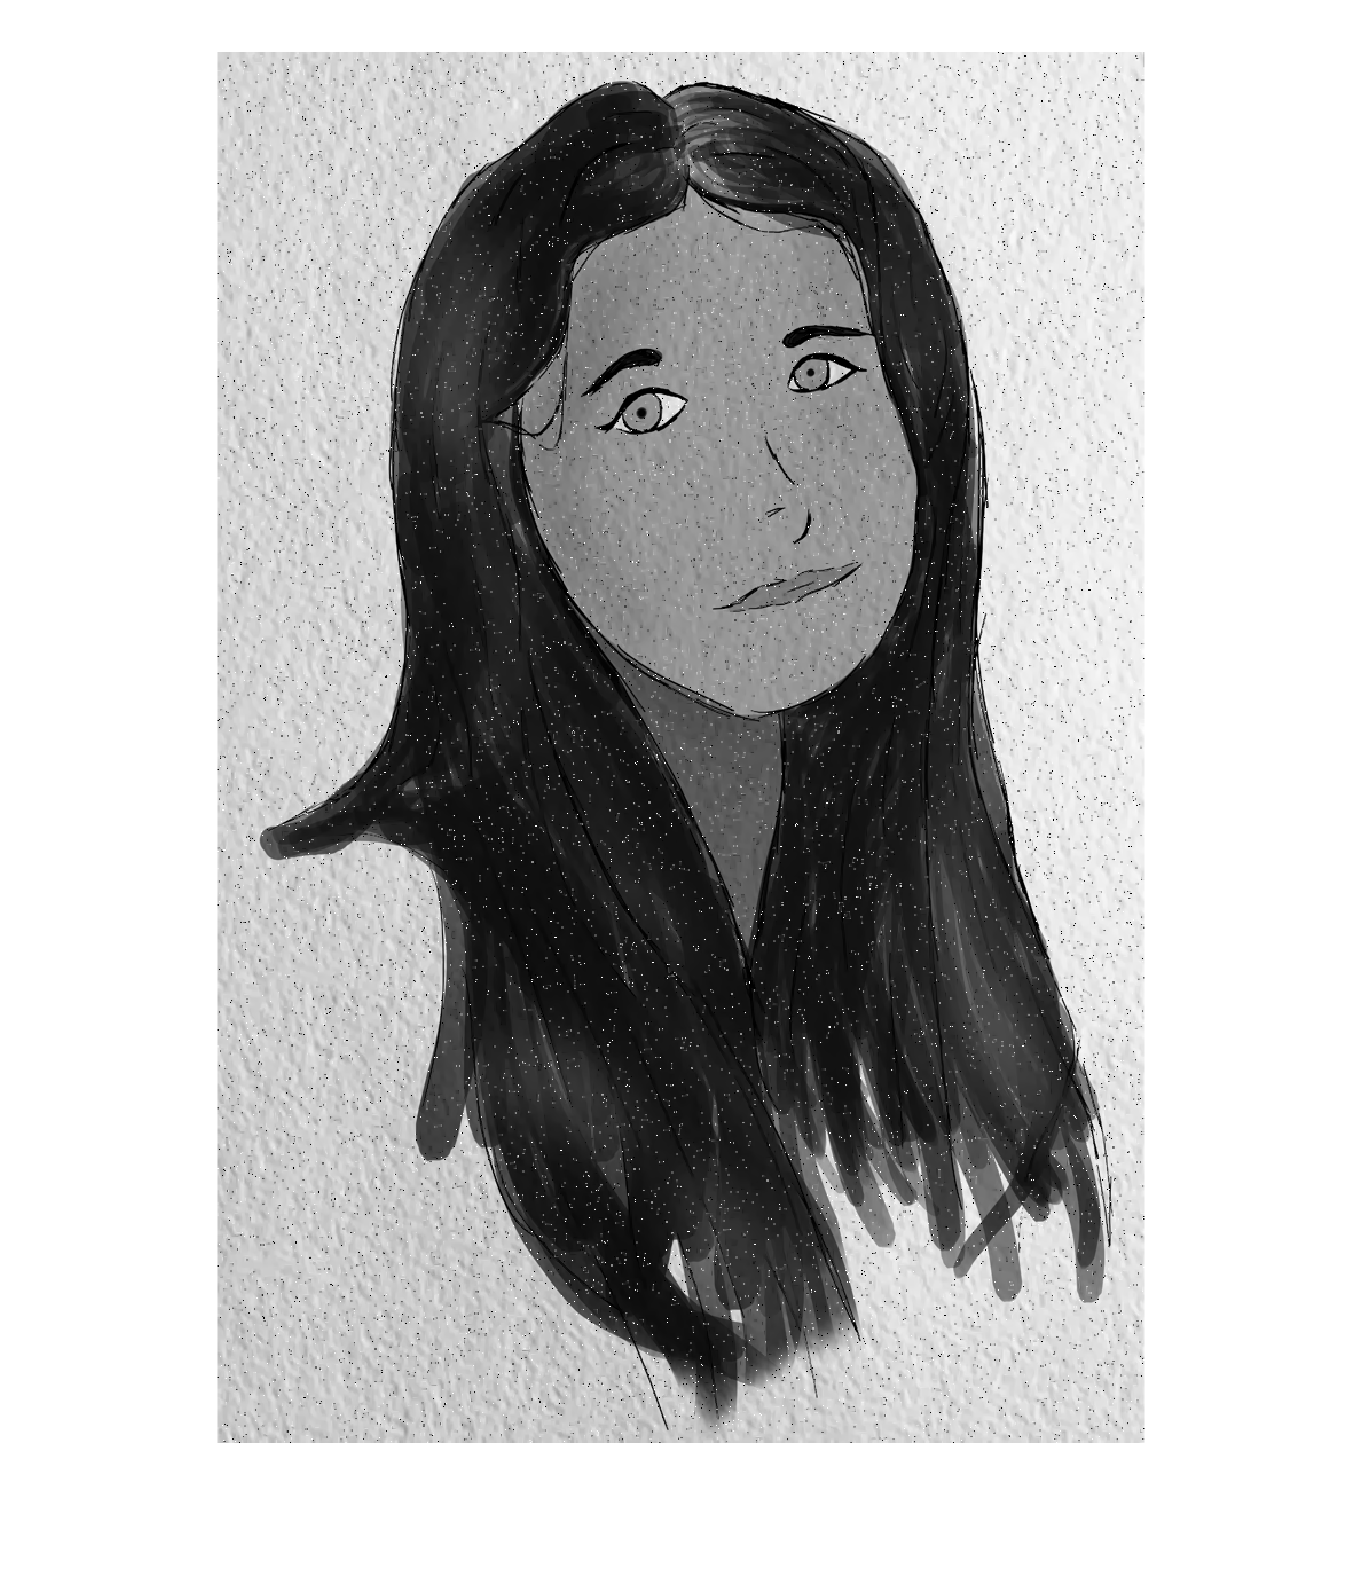
\includegraphics[scale=0.15,trim={3cm 3cm 0cm 0cm},clip]{Pictures/Esempi di utilizzo/Esempio 5/ami_filtrata_sigma0_5_resize.png}
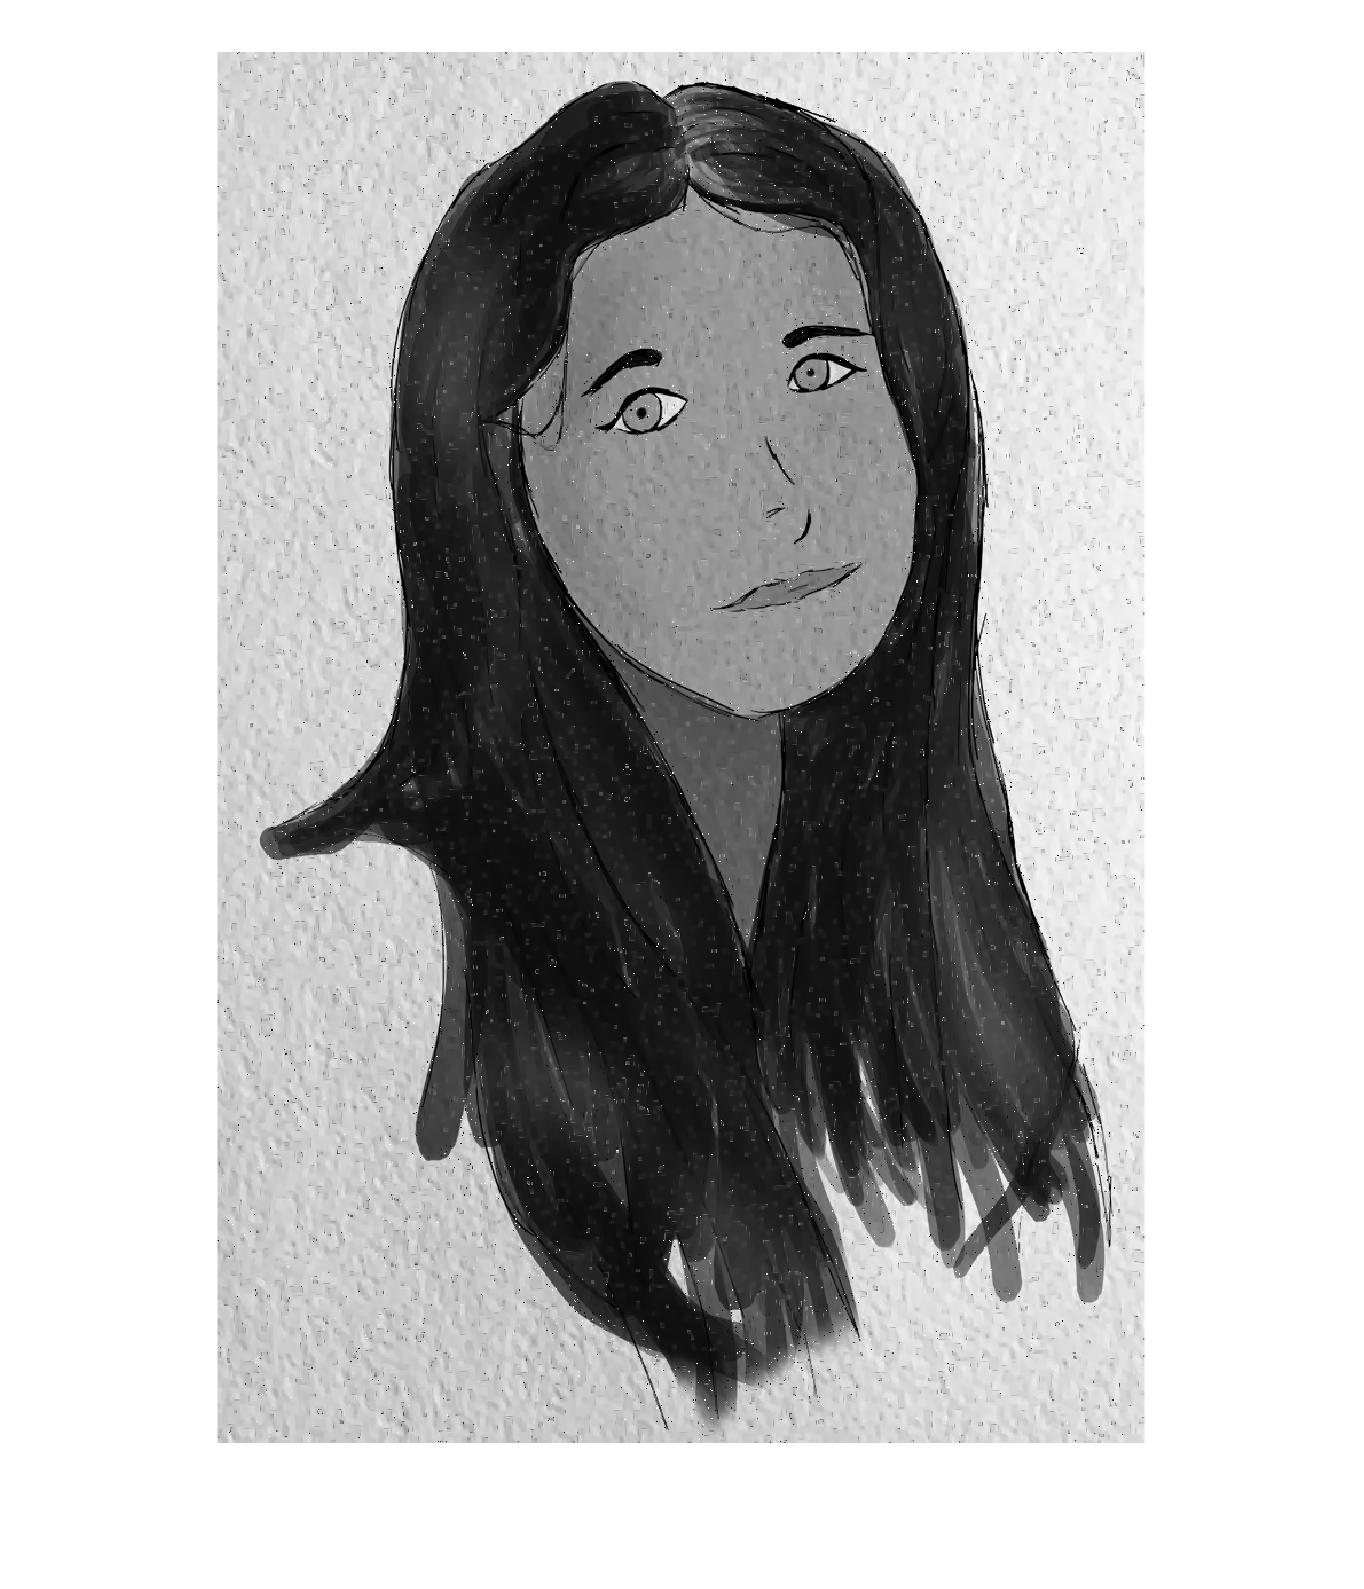
\includegraphics[scale=0.15,trim={0cm 0cm 3cm 0cm},clip]{Pictures/Esempi di utilizzo/Esempio 5/ami_filtrata_sigma1_resize.png}
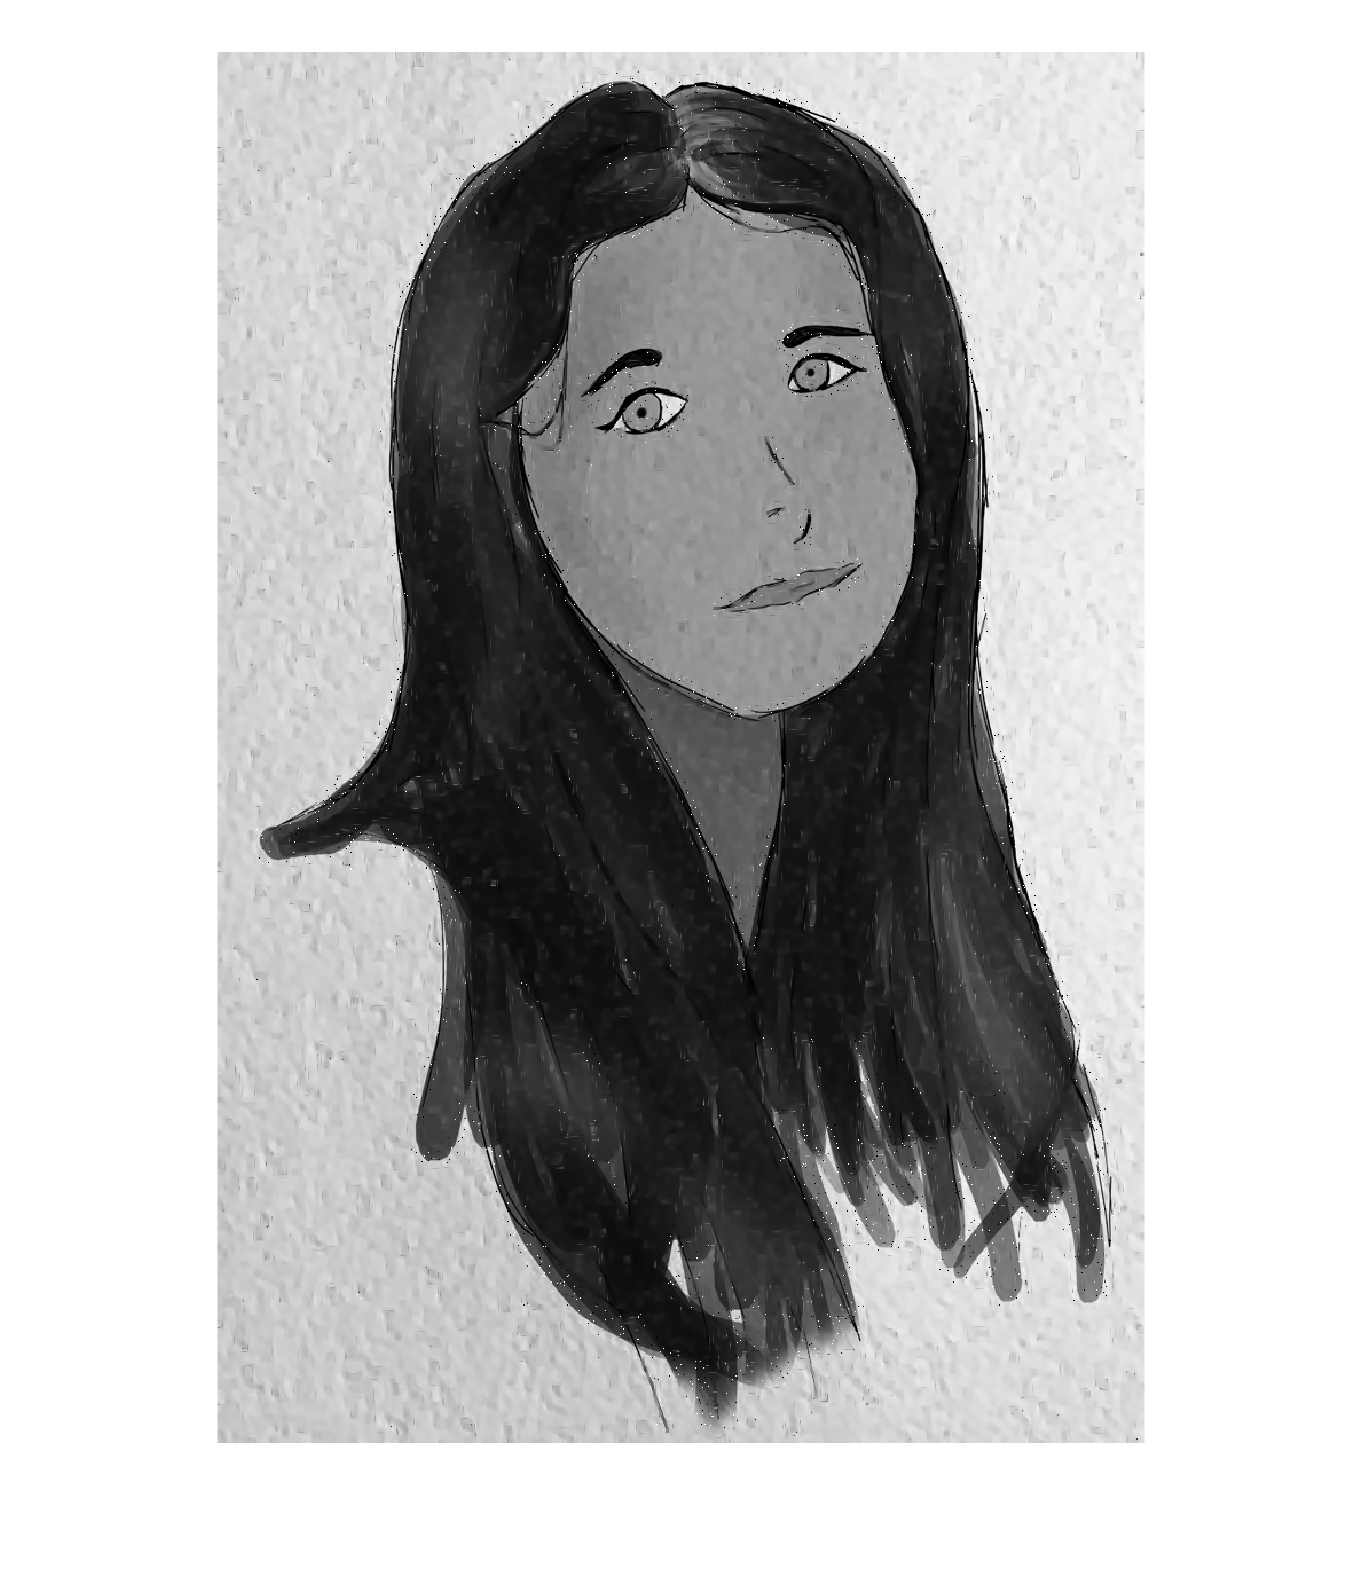
\includegraphics[scale=0.15,trim={3cm 0cm 0cm 0cm},clip]{Pictures/Esempi di utilizzo/Esempio 5/ami_filtrata_sigma2_resize.png}
\caption{In ordine: immagine con rumore, immagine filtrata con sigma=0.5, con sigma=1 e con sigma=2.}\label{fig:figura}
\end{figure} 
Anche in questo caso, come visto nell'esempio 3, bisogna fare attenzione a non impostare valori troppo alti. Nell'esempio 3 ce ne siamo preoccupati perchè il metodo prevede il calcolo \texttt{diff\_im = diff\_im + delta\_t*(cN.*nablaN + cS.*nablaS + cW.*nablaW + cE.*nablaE)} e si era detto che per garantire la stabilità numerica utilizziamo $delta\_t \in [0,\frac{1}{4}]$.
Ricordiamo adesso che per operare il filtraggio richiamiamo l'equazione del calore, che invece prevede il calcolo \texttt{u= u + sigma*dt*(u\_{xx}+u\_{yy})}, per cui per assicurare la stabilità numerica imponiamo anche $delta\_t*sigma \in[0,\frac{1}{4}]$, in accordo con quanto visto nella \textbf{Proposizione 2.1.1}. Vediamo ad esempio quali risultati otteniamo ponendo sigma=2, che abbiamo visto dare un buon risultato, e delta\_t=0.2.\\
Parametri:
\begin{itemize}
    \item num\_iter=20
    \item delta\_t=0.2
    \item c=0.5
    \item sigma=2
\end{itemize}

\begin{figure}[htb] \centering
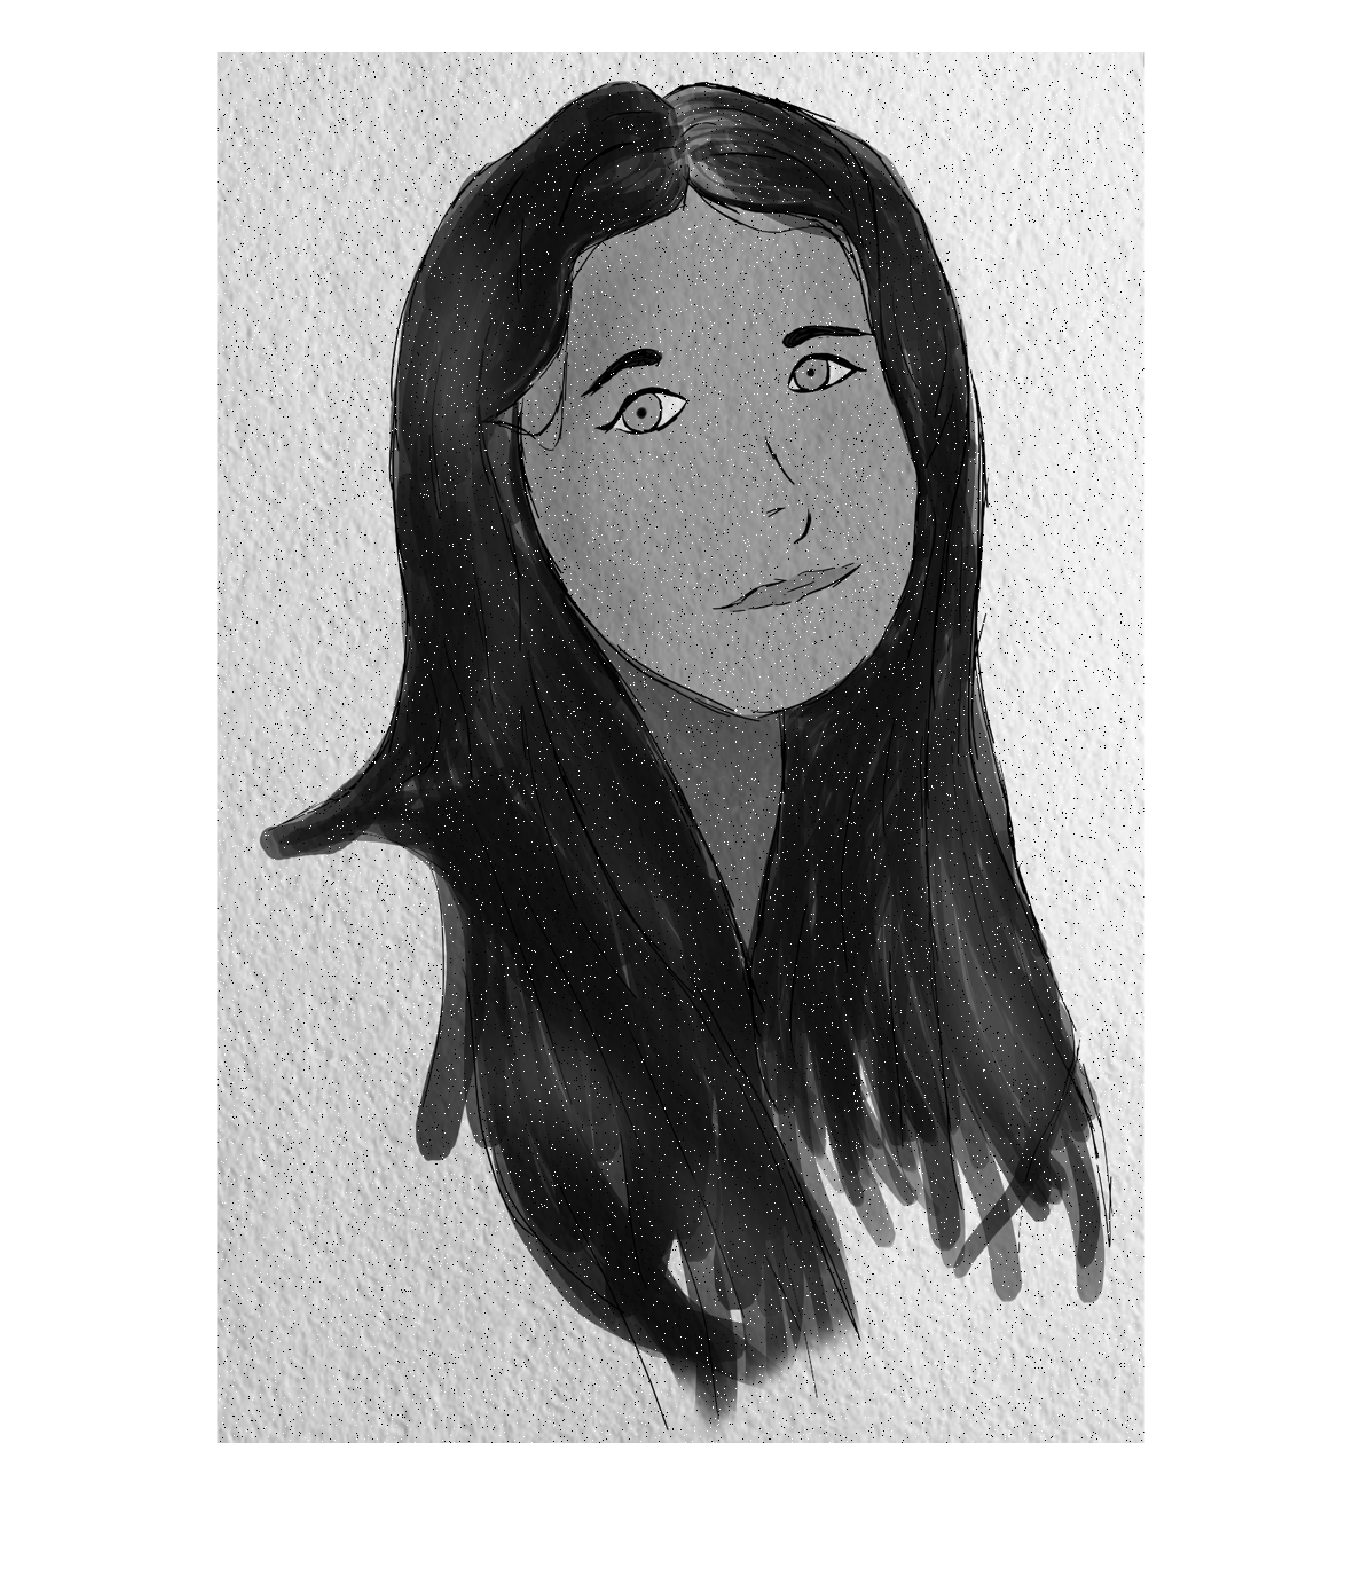
\includegraphics[scale=0.15,trim={3cm 0cm 3cm 0cm},clip]{Pictures/Esempi di utilizzo/Esempio 5/ami_originale_resize.png}
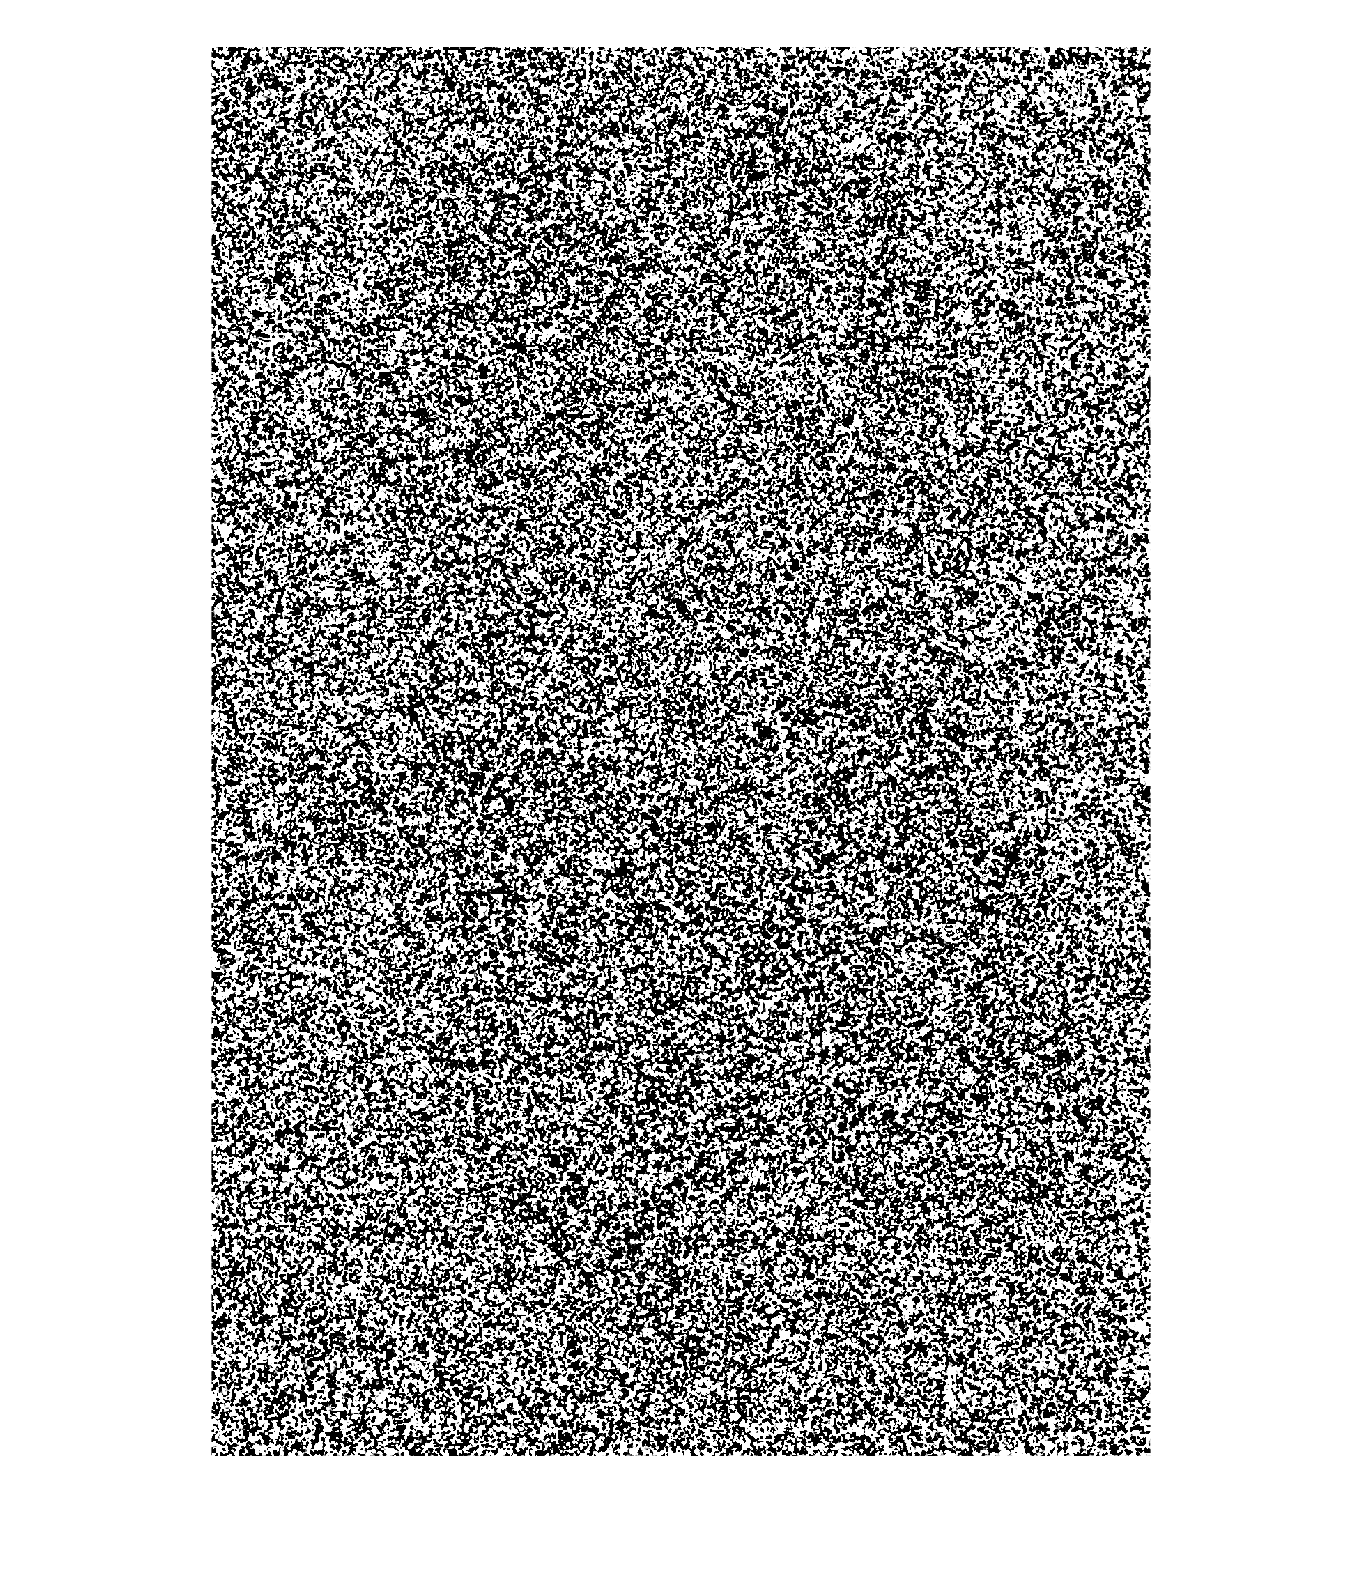
\includegraphics[scale=0.15,trim={3cm 0cm 3cm 0cm},clip]{Pictures/Esempi di utilizzo/Esempio 5/ami_calore_sigma2_deltat0_2_resize.png}
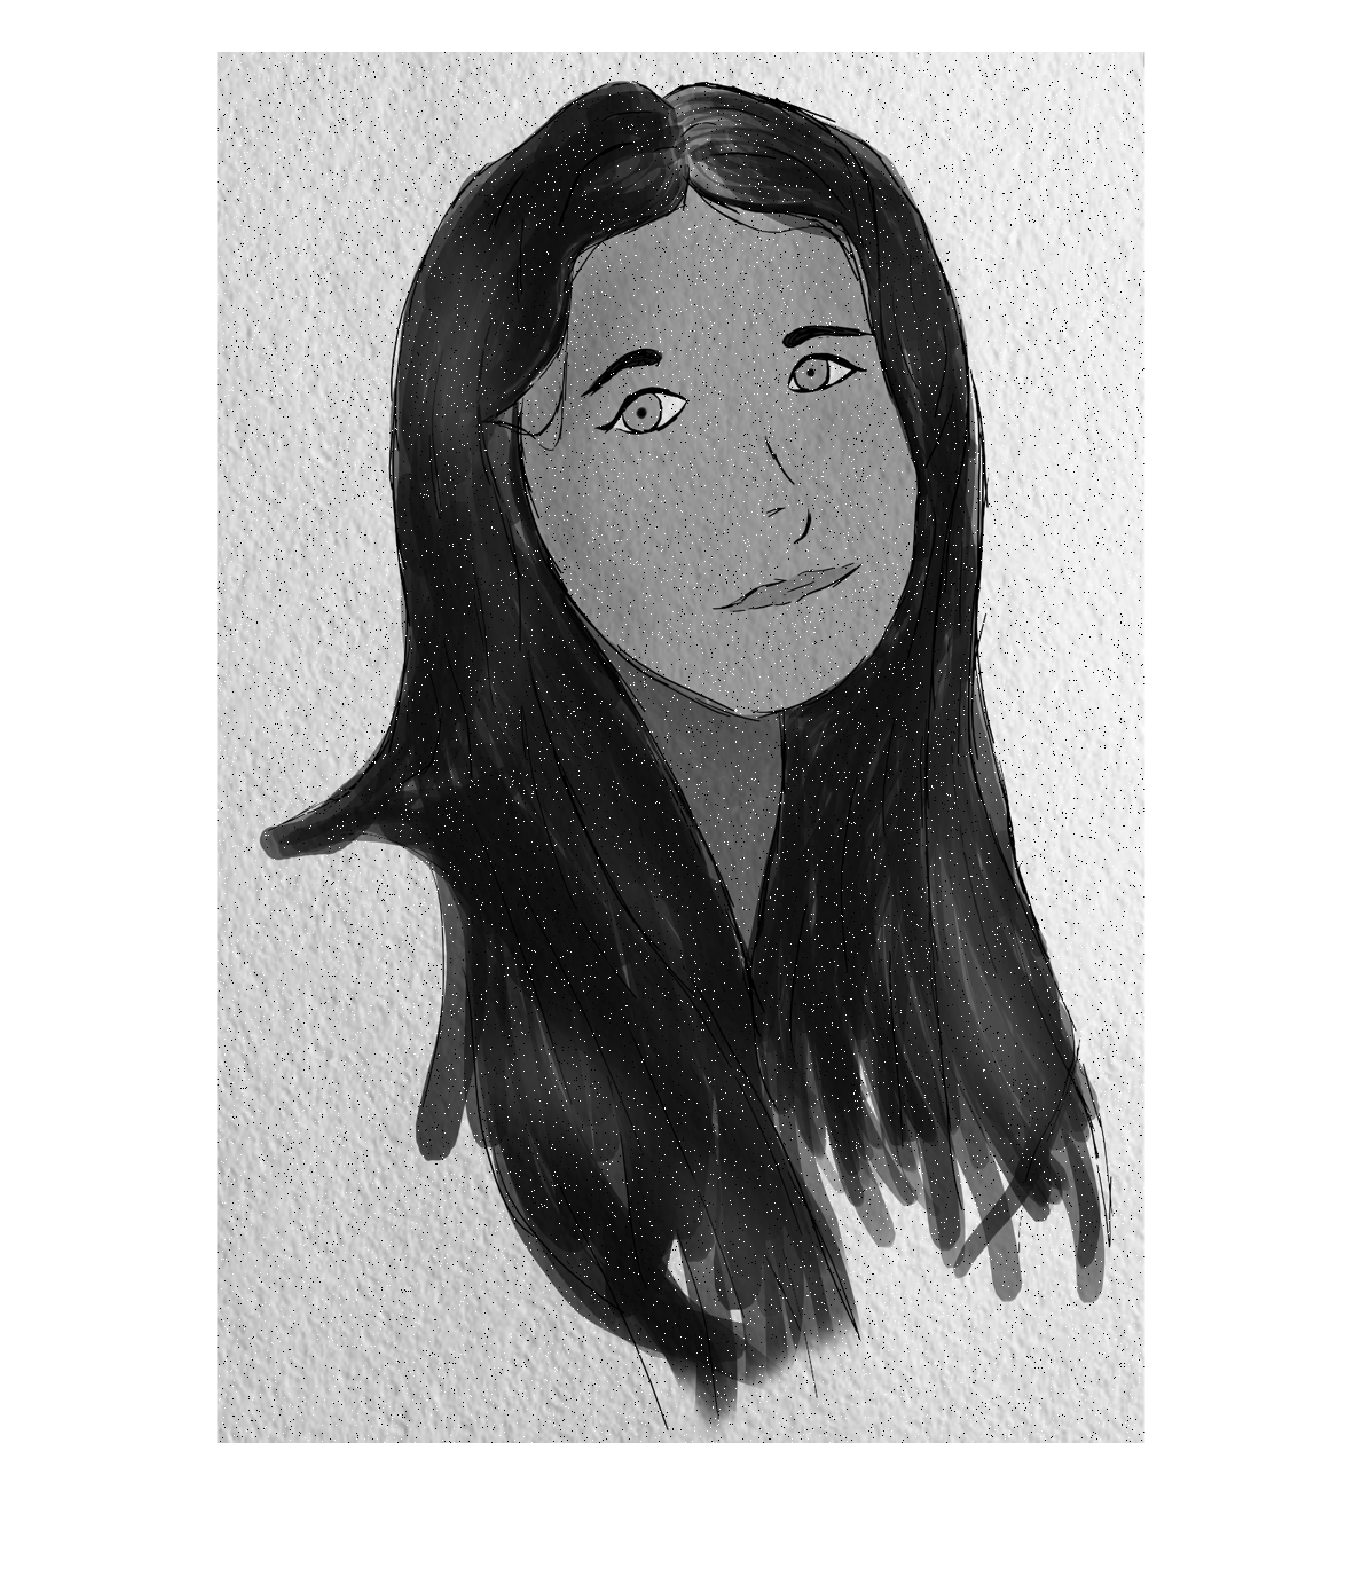
\includegraphics[scale=0.15,trim={3cm 0cm 3cm 0cm},clip]{Pictures/Esempi di utilizzo/Esempio 5/ami_filtrata_sigma2_deltat0_2_resize.png}
\caption{In ordine: immagine originale, immagine filtrata con equazione del calore e immagine filtrata con sigma=2.}\label{fig:figura}
\end{figure} 
Otteniamo quindi un'immagine quasi non filtrata, numericamente infatti troviamo:
\texttt{min(min([cN,cS,cW,cE]))=0} e \texttt{max(max([cN,cS,cW,cE]))=4.3775e-106}
riconosciamo quindi un appiattimento di c sullo 0.